\documentclass[twocolumn]{aastex62}
%\documentclass[iop,revtex4]{emulateapj}
\let\pwiflocal=\iffalse \let\pwifjournal=\iffalse
\usepackage{amsmath,amssymb}
\usepackage{epsfig}    
\usepackage{graphicx}    
\usepackage{lineno}
\usepackage{natbib}
\usepackage{bigints}
\usepackage[outdir=./]{epstopdf}

\usepackage[T1]{fontenc}
\pwifjournal\else
  \usepackage{microtype}
\fi

\pwifjournal\else
  \makeatletter
  \renewcommand\plotone[1]{%
    \centering \leavevmode \setlength{\plot@width}{0.95\linewidth}
    \includegraphics[width={\eps@scaling\plot@width}]{#1}%
  }%
  \makeatother
\fi


\makeatletter

\newcommand\@simpfx{http://simbad.u-strasbg.fr/simbad/sim-id?Ident=}

\newcommand\MakeObj[4][\@empty]{% [shortname]{ident}{url-escaped}{formalname}
  \pwifjournal%
    \expandafter\newcommand\csname pkgwobj@c@#2\endcsname[1]{\protect\object[#4]{##1}}%
  \else%
    \expandafter\newcommand\csname pkgwobj@c@#2\endcsname[1]{\href{\@simpfx #3}{##1}}%
  \fi%
  \expandafter\newcommand\csname pkgwobj@f#2\endcsname{#4}%
  \ifx\@empty#1%
    \expandafter\newcommand\csname pkgwobj@s#2\endcsname{#4}%
  \else%
    \expandafter\newcommand\csname pkgwobj@s#2\endcsname{#1}%
  \fi}%

\newcommand\MakeTrunc[2]{% {ident}{truncname}
  \expandafter\newcommand\csname pkgwobj@t#1\endcsname{#2}}%

\newcommand{\obj}[1]{%
  \expandafter\ifx\csname pkgwobj@c@#1\endcsname\relax%
    \textbf{[unknown object!]}%
  \else%
    \csname pkgwobj@c@#1\endcsname{\csname pkgwobj@s#1\endcsname}%
  \fi}
\newcommand{\objf}[1]{%
  \expandafter\ifx\csname pkgwobj@c@#1\endcsname\relax%
    \textbf{[unknown object!]}%
  \else%
    \csname pkgwobj@c@#1\endcsname{\csname pkgwobj@f#1\endcsname}%
  \fi}
\newcommand{\objt}[1]{%
  \expandafter\ifx\csname pkgwobj@c@#1\endcsname\relax%
    \textbf{[unknown object!]}%
  \else%
    \csname pkgwobj@c@#1\endcsname{\csname pkgwobj@t#1\endcsname}%
  \fi}

\makeatother


% Evil magic to patch natbib to only highlight the year paper refs, not the
% authors too; as seen in ApJ. From
% http://tex.stackexchange.com/questions/23227/.

\pwifjournal\else
  \usepackage{etoolbox}
  \makeatletter
  \patchcmd{\NAT@citex}
    {\@citea\NAT@hyper@{%
       \NAT@nmfmt{\NAT@nm}%
       \hyper@natlinkbreak{\NAT@aysep\NAT@spacechar}{\@citeb\@extra@b@citeb}%
       \NAT@date}}
    {\@citea\NAT@nmfmt{\NAT@nm}%
     \NAT@aysep\NAT@spacechar\NAT@hyper@{\NAT@date}}{}{}
  \patchcmd{\NAT@citex}
    {\@citea\NAT@hyper@{%
       \NAT@nmfmt{\NAT@nm}%
       \hyper@natlinkbreak{\NAT@spacechar\NAT@@open\if*#1*\else#1\NAT@spacechar\fi}%
         {\@citeb\@extra@b@citeb}%
       \NAT@date}}
    {\@citea\NAT@nmfmt{\NAT@nm}%
     \NAT@spacechar\NAT@@open\if*#1*\else#1\NAT@spacechar\fi\NAT@hyper@{\NAT@date}}
    {}{}
  \makeatother
\fi


% Object data

\providecommand{\eprint}[1]{\href{http://arxiv.org/abs/#1}{#1}}
\providecommand{\adsurl}[1]{\href{#1}{ADS}}
\newcommand{\mps}{m\,s$^{-1}$}
\providecommand{\icarus}{Icarus}
\newcommand{\vsini}{$v\sin{i_*}$}
\newcommand{\vdag}{(v)^\dagger}
\newcommand{\oxygen}{O$_2$}
\newcommand{\water}{H$_2$O}
\newcommand{\kepler}{{\it Kepler}}
\newcommand{\logg}{$log~g$ }
\newcommand{\metal}{[M/H]}
\newcommand{\um}{$\mu$m}
\newcommand{\fbol}{$F_{\mathrm{bol}}$}
\newcommand{\mbol}{$m_{\mathrm{bol}}$}
\newcommand{\Mbol}{$M_{\mathrm{bol}}$}
\newcommand{\rapsq}{$R_{ap}^2$}
\newcommand{\rchisq}{$\chi^2_{\nu}$}
\newcommand{\hipp}{{\it Hipparcos}}
\newcommand\teff{\ensuremath{T_\text{eff}}}
% utility

%\newcommand{\vdag}{(v)^\dagger}
%\newcommand{\oxygen}{O$_2$}
%\newcommand{\water}{H$_2$O}
%\newcommand{\kepler}{{\it Kepler}}
%\newcommand{\logg}{$log~g$ }
%\newcommand{\metal}{[M/H]}
%\newcommand{\um}{$\mu$m}
%\newcommand{\fbol}{$F_{\mathrm{bol}}$}
%\newcommand{\mbol}{$m_{\mathrm{bol}}$}
%\newcommand{\Mbol}{$M_{\mathrm{bol}}$}
%\newcommand{\rapsq}{$R_{ap}^2$}
%\newcommand{\rchisq}{$\chi^2_{\nu}$}
%\newcommand{\hipp}{{\it Hipparcos}}
%
%
%\newcommand\aafd{erg~s$^{-1}$~cm$^{-2}$~\AA$^{-1}$} % "AAngstrom flux density"
%\newcommand\amlt{$\alpha_{\rm MLT}$} % convective mixing length parameter
%\newcommand\apx{\ensuremath{\sim}}
%\newcommand\cgsflux{erg~s$^{-1}$~cm$^{-2}$}
%\newcommand\cgslum{erg~s$^{-1}$}
%\newcommand\chandra{\textit{Chandra}}
%\newcommand\citeeg[1]{\citep[\eg,][]{#1}}
%\newcommand\cps{ct~s$^{-1}$}
%\newcommand\dd{\ensuremath{\text{d}}}
%\newcommand\eg{\textit{e.g.}}
%\newcommand\etal{\textit{et~al.}}
%\newcommand\ewha{\ensuremath{\text{EW}(\ha)}}
%%\newcommand\fig[1]{Figure~\ref{f.#1}}
%\newcommand\ha{{\ensuremath{\text{H}\alpha}}}
%\newcommand\I{\mathcal{I}}
%\newcommand\ie{\textit{i.e.}}
\newcommand\kms{km~s$^{-1}$}
%\newcommand\ls{L$_\odot$}
%\newcommand\mj{M$_\text{J}$}
%\newcommand\ms{M$_\odot$}
%\newcommand\nupk{\ensuremath{\nu_\text{pk}}}
%\newcommand\percc{cm$^{-3}$}
%\newcommand\rcs{\ensuremath{\chi_r^2}}
%\newcommand\rj{R$_\text{J}$}
%\newcommand\sect[1]{Section~\ref{s.#1}}
%\newcommand\sherpa{\textsf{Sherpa}}
%\newcommand\sti{Stokes~$I$}
%\newcommand\stiv{Stokes~$I$ and~$V$}
%\newcommand\stv{Stokes~$V$}
%\newcommand\swift{\textit{Swift}}
%\newcommand\tb{\ensuremath{T_\text{b}}}
%\newcommand\tbl[1]{Table~\ref{t.#1}}
%\newcommand\teff{\ensuremath{T_\text{eff}}}
%\newcommand\todo[1]{\textcolor{red}{#1}}
%\newcommand\ujy{$\mu$Jy}
%\newcommand\ujybm{$\mu$Jy~bm$^{-1}$}
%\newcommand\uv{$u$\mbox{-}$v$}
%\newcommand\vsi{\ensuremath{v \sin i}}
%
%\newcommand\Lb{\ensuremath{L_\text{bol}}}
%\newcommand\Lh{\ensuremath{L_\ha}}
%\newcommand\Lr{\ensuremath{L_\text{R}}}
%\newcommand\sLr{\ensuremath{L_{\nu,\text{R}}}}
%\newcommand\Lu{\ensuremath{L_\text{UVW1}}}
%\newcommand\Lx{\ensuremath{L_\text{X}}}
%\newcommand\Lxf{\ensuremath{L_{\text{X},f}}}
%\newcommand\Lxq{\ensuremath{L_{\text{X},q}}}
%\newcommand\lb{\ensuremath{[\Lb]}}
%\newcommand\lh{\ensuremath{[\Lh]}}
%\newcommand\lr{\ensuremath{[\Lr]}}
%\newcommand\slr{\ensuremath{[\sLr]}}
%\newcommand\lu{\ensuremath{[\Lu]}}
%\newcommand\lx{\ensuremath{[\Lx]}}
%\newcommand\lxf{\ensuremath{[\Lxf]}}
%\newcommand\lxq{\ensuremath{[\Lxq]}}
%\newcommand\lhlb{\ensuremath{[\Lh/\Lb]}}
%\newcommand\lrlb{\ensuremath{[\Lr/\Lb]}}
%\newcommand\lulb{\ensuremath{[\Lu/\Lb]}}
%\newcommand\lxlb{\ensuremath{[\Lx/\Lb]}}
%\newcommand\lxflb{\ensuremath{[\Lxf/\Lb]}}
%\newcommand\lxqlb{\ensuremath{[\Lxq/\Lb]}}
%\newcommand\slrlb{\ensuremath{[\sLr/\Lb]}}
%\newcommand\slrlx{\ensuremath{[\sLr/\Lx]}}
%\newcommand\slrlxf{\ensuremath{[\sLr/\Lxf]}}
%\newcommand\slrlxq{\ensuremath{[\sLr/\Lxq]}}

\usepackage[outdir=./]{epstopdf}

\newcommand{\ktwo}{{\it K2}}
\newcommand{\av}{$A_V$}
\newcommand{\mks}{$M_{K_S}$}
\newcommand{\mmk}{$M_{K_S}-M_*$}
\usepackage{mathrsfs}
%\usepackage[colorlinks=true,urlcolor=blue,citecolor=black]{hyperref}
%\usepackage{xcolor}
%\usepackage[colorlinks = true,
%            linkcolor = blue,
%            urlcolor  = blue,
%            citecolor = blue,
%            anchorcolor = blue]{hyperref}
%\newcommand{\href}{\href}%
%\newcommand{\href}[3][blue]{\href{#2}{\color{#1}{#3}}}%
%\slugcomment{To be Submitted to ApJ}

\shorttitle{M dwarf mass-luminosity relation}
\shortauthors{Mann et al.}
\submitjournal{The Astrophysical Journal}


\bibliographystyle{apj}


\begin{document}
 
\title{Weighing the Stars I:\\ The mass-luminosity relation from 0.70$M_\odot$ to 0.075$M_\odot$
%$M_*$-$M_{K_S}$ relation from 0.7$M_\odot$ to 0.075$M_\odot$%. \\
%or \\
%How to constrain your M dwarf II: \\
 %the $M_*$-$M_{K_S}$ relation from 0.7$M_\odot$ to 0.075$M_\odot$
 } 
 

\correspondingauthor{Andrew W. Mann}
\email{mann.andrew.w@gmail.com}

\author[0000-0003-3654-1602]{Andrew W. Mann}
\altaffiliation{Hubble Fellow}
\affiliation{Columbia University, Department of Astronomy, 550 West 120th Street, New York, NY 10027}
\affiliation{Department of Physics and Astronomy, University of North Carolina at Chapel Hill, Chapel Hill, NC 27599-3255, USA}

\author[0000-0001-9823-1445]{Trent Dupuy}
\affiliation{Gemini Observatory, Northern Operations Center, 670 N. Aohoku Place, Hilo, HI 96720, USA}
 
\author[0000-0001-9811-568X]{Adam Kraus}
\affiliation{Department of Astronomy, The University of Texas at Austin, Austin, TX 78712, USA}

\author[0000-0002-5258-6846]{Eric Gaidos}
\affiliation{Department of Geology \& Geophysics, University of Hawaii at M\={a}noa, Honolulu, Hawaii 96822 USA}

\author[0000-0001-9982-1332]{Aaron Rizzuto}
\altaffiliation{51 Peg b Fellow}
\affiliation{Department of Astronomy, The University of Texas at Austin, Austin, TX 78712, USA}

\author[0000-0002-6194-043X]{Michael Ireland}%
\affiliation{Research School of Astronomy \& Astrophysics, Australian National University, Canberra ACT 2611, Australia}

\author[0000-0003-4142-9842]{Megan Ansdell}%
\affiliation{Department of Astronomy, University of California at Berkeley, Berkeley, CA 94720, USA}

\author{Jean-Luc Beuzit}
\affiliation{Observatoire de Grenoble, Institut de Planetologie et d'Astrophysique de Grenoble, BP 53, 38041 Grenoble Cedex 9, France}

\author[0000-0001-7730-2240]{Jason Dittmann}
\affiliation{Harvard-Smithsonian Center for Astrophysics, 60 Garden St., Cambridge, MA, 02138}

\author[0000-0002-6879-3639]{Chao-Ling Hung}
\affiliation{Department  of  Physics, Manhattan  College,  4513  Manhattan College Parkway, Riverdale, NY 10471, USA}

\author[0000-0002-8332-8516]{Samuel Factor}
\affiliation{Department of Astronomy, The University of Texas at Austin, Austin, TX 78712, USA}

\author[0000-0003-0536-4607]{Thierry Forveille}
\affiliation{Observatoire de Grenoble, Institut de Planetologie et d'Astrophysique de Grenoble, BP 53, 38041 Grenoble Cedex 9, France}

\author[0000-0003-2232-7664]{Michael Liu}
\affiliation{Institute for Astronomy, University of Hawai`i at M\={a}noa, Honolulu, HI 96822, USA}

\author[0000-0001-6301-896X]{Raquel Martinez}
\affiliation{Department of Astronomy, The University of Texas at Austin, Austin, TX 78712, USA}

\watermark{Draft}

%\author{
%Andrew W. Mann\altaffilmark{\ut,\col,\hub}, 
%Trent Dupuy\altaffilmark{\ut,\gem}, 
%Adam Kraus\altaffilmark{\ut},
%Eric Gaidos\altaffilmark{\geo},
%Aaron Rizzuto\altaffilmark{\ut,\peg},
%Michael Ireland\altaffilmark{\aus},
%Megan Ansdell\altaffilmark{\ifa,\ber},
%Jean-Luc Beuzit\altaffilmark{\gren},
%Jason Dittmann\altaffilmark{\har},
%Chao-Ling Hung\altaffilmark{\man},
%Samuel Factor\altaffilmark{\ut},
%Thierry Forveille\altaffilmark{\gren},
%Michael Liu \altaffilmark{\ifa},
%Raquel Martinez\altaffilmark{\ut}
%}
%
%\email{mann.andrew.w@gmail.com}
%
%\newcommand\ut{1}
%\newcommand\col{2}
%\newcommand\hub{3}
%\newcommand{\gem}{4}
%\newcommand\geo{5}
%\newcommand\peg{6}
%\newcommand\aus{7}
%\newcommand\ifa{8}
%\newcommand{\ber}{9}
%\newcommand\gren{10}
%\newcommand\har{11}
%\newcommand{\man}{12}
%
%\altaffiltext{\ut}{Department of Astronomy, The University of Texas at Austin, Austin, TX 78712, USA}
%\altaffiltext{\col}{Columbia University, Department of Astronomy, 550 West 120th Street, New York, NY 10027}
%\altaffiltext{\hub}{Hubble Fellow}
%\altaffiltext{\gem}{Gemini Observatory, Northern Operations Center, 670 N. Aohoku Place, Hilo, HI 96720, USA}
%\altaffiltext{\geo}{Department of Geology \& Geophysics, University of Hawaii at M\={a}noa, Honolulu, Hawaii 96822 USA}
%\altaffiltext{\peg}{51 Peg b Fellow}
%\altaffiltext{\aus}{Research School of Astronomy \& Astrophysics, Australian National University, Canberra ACT 2611, Australia}
%\altaffiltext{\ifa}{Institute for Astronomy, University of Hawai`i at M\={a}noa, Honolulu, HI 96822, USA}
%\altaffiltext{\ber}{Department of Astronomy, University of California at Berkeley, Berkeley, CA 94720, USA}
%\altaffiltext{\gren}{Observatoire de Grenoble, Institut de Planetologie et d'Astrophysique de Grenoble, BP 53, 38041 Grenoble Cedex 9, France}
%\altaffiltext{\har}{Harvard-Smithsonian Center for Astrophysics, 60 Garden St., Cambridge, MA, 02138}
%\altaffiltext{\man}{Department  of  Physics, Manhattan  College,  4513  Manhattan College Parkway, Riverdale, NY 10471}


\begin{abstract}
The mass-luminosity relation for late-type stars has long been a critical tool for both estimating stellar masses and testing evolutionary models. New methods to measure the metallicities of M dwarfs, the availability of {\it Gaia} parallaxes, an increasing number of benchmark binaries near the hydrogen burning limit, and the need for higher-precision masses for M dwarfs in the Solar neighborhood all motivate revisiting existing relations. Here we present an empirical relation between \mks\ and $M_*$ spanning 0.70$M_\odot$ down to the hydrogen burning limit ($\simeq0.075M_\odot$). The relation is calibrated from 61 nearby binary systems, whose orbits we determine using a a combination of our own monitoring with NIRC2 on Keck, archival adaptive optics data, and astrometry from the literature. We use these data to determine total masses to better than 1\% in the best cases (median precision of 6.4\%). Joining these masses with resolved \mks\ magnitudes for binary component stars, we fit an empirical \mmk\ relation that can be used to predict masses to 2-3\% for $0.18M_\odot<M_*<0.70M_\odot$, and 3-6\% for $0.075M_\odot<M_*<0.18M_\odot$. Our resulting relation is mostly consistent with earlier work, and deviations are explainable by differences in the input sample. We find [Fe/H] has a weak effect on the \mmk\ for the range of metallicities expected in the Solar neighborhood ($\simeq$1\% change in $M_*$), but may exceed uncertainties in the relation ($>3\%$) for subdwarfs. Our results also suggest that evolutionary models likely overestimate the role of [Fe/H] on the \mmk\ relation, but the difference is not significant with the current sample. %Future studies including a sample of cool subdwarf binaries will be needed to better explore the role of [Fe/H].
\end{abstract}

\keywords{stars: fundamental parameters; stars: low-mass; stars: luminosity function, mass function}
\NewPageAfterKeywords

% without latex:
%The mass-luminosity relation for late-type stars has been a critical tool for both measuring stellar masses and testing evolutionary models for decades. It is now possible to significantly improve on past relations thanks to new methods to measure the metallicity of M dwarfs, the availability of {\it Gaia} parallaxes, and an increasing number of benchmark binaries near the hydrogen burning limit. Here we present an empirical relation between \mks\ and $M_*$ calibrated using astrometric binaries from 0.70$M_\odot$ down to the hydrogen burning limit ($\simeq0.075M_\odot$). The relation is built from 61 nearby binary systems, whose orbits we determine using a a combination of our own monitoring with NIRC2 on Keck, archive adaptive optics data, and astrometry measurements in the literature. We use these data to determine total masses for each system and \mks\ magnitudes for each component, which we use to fit an empirical \mmk\ relation. System mass are determined to better than 1\% in the best cases (median precision of 6.4\%). The resulting relation can be used to predict masses to 2-3\% over for $M_*>0.18M_\odot$, and 3-6\% down to the hydrogen burning limit. Using empirically calibrated metallicities, we attempt to explore the role of [Fe/H] on the \mmk\. We find that the effect is likely small for the range of metallicities expected in the Solar neighborhood ($\simeq$1\% change in $M_*$), but may exceed uncertainties in the relation ($>3\%$) for dwarfs with [Fe/H]$\ll-0.5$. Our results also suggest that evolutionary models likely overestimate the role of [Fe/H] on the relation, but the difference is not significant at this point. Future studies including a sample of subdwarf binaries will be needed to better explore the role of [Fe/H].

%\section{To do list:}
%\begin{itemize}
%\item ORCIDs from Co-authors
%\item Giant table of all input astrometry.
%\item Full corner plot for one sample system
%\item personal corner plot instead of DFM's?
%\item Very long MCMC run (1 million)
%\end{itemize}


\section{Introduction}\label{sec:intro}
Over the past decade, M dwarfs have become critically important across a wide range of astrophysics. On the small scale, M dwarfs have become attractive targets for the identification and characterization of exoplanets. The small size, low mass, and low luminosity of late-type dwarfs facilitates the discovery of exoplanets, particularly planets that are small \citep[e.g.][]{Muirhead2012,Martinez:2017aa,Mann:2018}, young \citep[e.g.,][]{2012ApJ...753..142B,Mann2016b}, and/or in their circumstellar habitable-zone \citep[e.g.,][]{Tarter2007,Shields:2016aa,2017Natur.544..333D}. Close-in, rocky planets are also significantly more common around M dwarfs than their Sun-like counterparts \citep{Dressing2013,2013PNAS..11019273P,Mulders2015,Gaidos2016b}, and are more likely to harbor close-in multi-planet systems \citep[e.g.,][]{Muirhead2015,Ballard2016}. 

Like planets, studies of Galactic properties are inexorably linked to the properties of their most numerous constituents \citep[$>$70\% of stars in the Solar neighborhood are M dwarfs,][]{Henry:1994fk,Reid:2004lr}. Late-type dwarfs weigh heavily on the Galactic mass function \citep[e.g.,][]{Covey:2008lr}, and are useful probes of the Milky Way's structure \citep[e.g.,][]{2008ApJ...673..864J,2017ApJ...843..141F}, kinematics \citep[e.g.,][]{2007AJ....134.2418B,2015RAA....15..860Y} and chemical evolution \citep{Woolf:2012lr,2015AJ....149..140H}. 

Late-type stars also play an important role on extragalactic and potentially cosmological scales. Although K and M dwarfs are much fainter than their higher-mass counterparts, they are numerous enough to impact the integrated light of many massive galaxies, making their properties an essential component of the initial mass function \citep[e.g.,][]{2012ApJ...747...69C,2016ApJ...821...39M} and mass-to-light ratio \citep{2015MNRAS.452L..21S} in nearby galaxies. Recent non-detection of Type Ia supernovae progenitors have shifted the field from single-degenerate origins (evolved star and a white dwarf) towards a double-degenerate model (two white dwarfs), however, single degenerate models with an M dwarf and a white dwarf are still plausible \citep{2012ApJ...758..123W}. 

For all these areas of research, it is essential that we have a method to estimate the masses of late type dwarfs, as well as a means to test methods on which M dwarf parameters are determined. For stars lacking a precise distance, most studies depend on evolutionary models to derive masses \citep[e.g.,][]{Muirhead2012a,2012ApJ...747...69C}. However, differences between empirical and model-predicted mass-radius and radius-luminosity relations for late-type stars \citep[e.g.,][]{Boyajian2012,Feiden2012a} raise concerns about the reliability of model-based masses. Further, the masses derived depend on both the model grid used \citep{Spada2013,MIST1}, and the observed parameter over which the interpolation is done \citep[e.g., color versus luminosity,][]{Mann:2012,Mann2015b}. Ultimately, these models need to be tested, and if necessary, refined. 

In a case where the target M dwarf has a precise distance, it is common to use a relation between mass and luminosity \citep[e.g.,][]{Henry:1993fk, Delfosse2000}. These relations are usually calibrated empirically using binaries, which have masses determined from long-term astrometric and/or spectroscopic monitoring of their orbits. Combined with a parallax and component magnitudes for each system, it is then possible to fit for a relation between absolute magnitude (a proxy for total luminosity) and stellar mass. 

The empirical mass-luminosity relations of \citet{Henry:1993fk} and \citet{Delfosse2000} provide mass determinations with $\simeq$10\% precision, with more recent improvements by \citet{Benedict2016}. As fields that rely on M dwarf parameters have pushed to higher precision, there has been need for proportionately improved precision on M dwarf masses. With he arrival of {\it Gaia} parallaxes late-type dwarfs even beyond the Solar neighborhood will have $<1\%$ parallaxes, making scatter in the \mmk\ relation the primary source of error. In addition to the need for better precision, all relations have gaps in their calibration sample, particularly below $0.1M_\odot$. Further, as these studies push to samples that are not well represented in the Solar neighborhood, it has become critical to understand systematics in the relation (e.g., metallicity, age, and activity). As methods to measure precise spectroscopic metallicities of M dwarfs have only recently become possible recently \citep[e.g.,][]{2010ApJ...720L.113R,2014A&A...568A.121N}, previous studies were unable to empirically study the role metallicity on the mass-luminosity relation. 

Here we present a revised empirical relation between $M_*$ and $M_{K_S}$ spanning almost an order of magnitude, from 0.075$M_\odot$ to 0.70$M_\odot$. The relation is built on orbital fits to visual binaries from a combination of adaptive optics imaging and astrometric measurements in the literature. In Section~\ref{sec:targets} we detail our selection of nearby late-type binaries with orbits amenable to mass determinations. We overview our astrometric and spectroscopic observations in Section~\ref{sec:obs}, including those from data archives and the literature. Our orbit-fitting procedure is explained in Section~\ref{sec:orbit}. We describe our method to determine other parameters of each system ([Fe/H], distance, and \mks) in Section~\ref{sec:params}. Our method and results from fitting the \mmk\ relation is described in Section~\ref{sec:relation}, including an analysis of the errors as a function of \mks\ and a detailed look at the effects of [Fe/H]. We compare our results to that of earlier relations in Section~\ref{sec:other}. We conclude in Section~\ref{sec:discussion} with a brief summary, and a discussion of the important caveats and complications to consider when using our relation, as well as future directions we are taking to expand on the work given here.

 {\it If you want to use the relations in this manuscript, we advise at least reading Section~\ref{sec:caveats} to understand the potential limitations of our provided \href{https://github.com/awmann/M_-M_K-}{program and posteriors}.}


\section{Target Selection}\label{sec:targets}

Our initial list of late-type binaries was built by cross-matching catalogs of nearby M dwarfs \citep{Lepine:2013, Gaidos2014, 2014ApJ...784..156D,Winters2015}, with the fourth catalog of interferometric measurements of binary stars \citep[INT4,][]{Hartkopf:2001}, and adaptive optics (AO) images from the Keck Observatory Archive (KOA). As part of this cross-match, we also included targets matching the M dwarf selection criteria of \citet{Gaidos2014}, but with a bluer ($V-J>2$) color cut to incorporate additional late-K dwarfs. We kept any binaries with separations less than 5\arcsec. We then added in other known late-type binaries from \citet{2008MNRAS.384..150L}, \citet{Janson2012}, \citet{2014ApJ...789..102J}, and \citet{Ward-Duong2015}. This provided a list of more than 300 systems.

From here we selected those for which we expect to be able to obtain a precise orbit on a reasonable (few year) timescale. We assumed the average of available separation measurements represented the typical semi-major axis. We then identified systems for which we would have at least 30\% of the orbit within the two years of our orbital monitoring program with Keck. This cut accounted for existing data. As a result, long-period binaries with extensive previous observations were included, depending on the baseline available, while those with only a single epoch would generally need to have orbits of $\ll$10 years to be observed. After this cut we were left with 125 systems. With the exception of 38 systems in the far South ($\delta<-30^\circ$, outside the range of Keck), all of these were included in our initial observing queue.

We removed 21 systems from our analysis because of an unresolved tertiary (or quaternary) component noted in the literature \citep[e.g.,][]{2010ApJ...720.1727L,2002A&A...382..118T,2018ApJS..235....6T}. In their current form, such systems are not useful for our analysis, as we have no $\Delta K$ magnitudes or mass ratios for the unresolved components. Since many of these are double- or triple-lined systems, it is possible to recover their parameters with multi-epoch radial velocities, and some systems already have the necessary data in the literature \citep[e.g.,][]{Sgr2000}. We are actively monitoring these systems with high-resolution near-infrared spectrographs \citep{2010SPIE.7735E..1MY,Park2014,2012SPIE.8446E..2CR}, but they are excluded from the analysis done here. Triples where the third component is more distant (and well resolved) were retained.

A total of 18 systems were flagged as young, all of which were tagged to nearby young moving groups or clusters \citep{Shkolnik2012, Kraus2014, Gagne2014, Malo2014a, Gagne2015, 2017AJ....153...95R, 2017AJ....154...69S, Rizzuto2017,2018MNRAS.475.2955L}. We continued to monitor these targets even after flagging them as young, but they were not included in the analysis for this paper. Many of these are expected to be pre-main-sequence stars and hence will not follow the same mass-luminosity relation. Even for those that are on the main-sequence, such young M dwarfs may have higher luminosities for a given mass \citep[e.g.,][]{2015ApJ...807....3K,Stassun2012,Somers2017}. These young systems will be the subject of a future study into the effects of age and activity on the parameters of M dwarfs. 

After the completion of our observing program, we removed targets for which we had $<$30\% of the orbit or fewer than six unique measurement epochs. We attempted to fit orbits of the remaining 70 systems (Section~\ref{sec:orbit}). Seven of the orbits fits failed to converge, mostly because their semi-major axes were much larger than expected (e.g., eccentric systems caught near periapsis). An additional 14 were removed because the derived mass for the system was too imprecise (errors $>$25\%) to be useful. Most of these 14 were systems with a poor or no parallax. This left us with 52 binaries (104 stars).

We added in nine targets with orbits from \citet{Dupuy2017}, primarily to fill in the sample around the end of the M dwarf sequence. These nine were selected because they are massive enough to sustain hydrogen fusion and satisfy all our other selection criteria. Systems from \citet{Dupuy2017} also had their orbits fit using a nearly identical method to our own, often using similar or identical data sources and observational methods (primarily Keck/NIRC2). 

Basic parameters of the final 61 systems included in our analysis are given in Table~\ref{tab:sample}.

\section{Observations and Data Reduction}\label{sec:obs} 

\subsection{Adaptive Optics Imaging}\label{sec:ao}

We analyzed a mix of AO data from our own program with NIRC2/Keck, and images from the archives of Keck, the Canada France Hawaii Telescope (CFHT), the Very Large Telescope, and Gemini observatory. In general we analyzed all usable (e.g., non saturated, components resolved) regardless of observing mode and filter. For our analysis, we considered a single `epoch' all data taken in a single night for a given target and filter. 

We separate the observations and reduction by instrument/telescope below. The full list of astrometry and contrast measurements is given in Table~\ref{tab:astrom}, sorted by target. 

\subsubsection{Keck II/NIRC2 Imaging and Masking}

Between March 2002 and November 2017, 48 of our targets were observed for a total of 166 epochs, all using the facility AO imager, NIRC2, on Keck II atop Maunakea. The majority of these data ($>100$ observations) were taken as part of our long-term monitoring program from June 2015 to November 2017. The rest of these observations were downloaded from the Keck Observatory Archive (KOA). For our observations, we always used the vertical angle mode and the narrow camera. Depending on brightness and conditions, imaging was usually taken with either the $K'$ or $K_{\rm{cont}}$ filters, and non-redundant aperture masking (NRM) was always taken using the 9-hole mask and $K'$ filter. After acquiring the target and allowing the AO loops to close, we took four to 10 images or 6-8 interferograms, adjusting coadds and integration time based on the brightness of the target. %As most of our targets are bright, observations were generally taking using the Natural Guide Star (NGS) system \citep{2000PASP..112..315W}, only utilizing the Laser Guide Star (LGS) mode for the faintest ($R\gtrsim13$) targets or in mixed conditions.

NIRC2 data taken from the archive comprised a wide range of observing modes, filters, and cameras, although the majority was taken with the narrow camera and one of the $H$- or $K$-band filters. We included nearly all data with a clear detection of both binary components independent of the observing setup. Archive data was taken between March 2002 up to November 2015. We discarded saturated images, those taken with the coronagraph atop one or both binary components, and those with extremely poor AO correction. 

The same basic data reduction was applied to both observations from our own program and those from the archive, following the procedure from \citet{Kraus2016a}. To briefly summarize, we linearized each frame then dark and flat corrected using calibration data taken the same night. In cases where no appropriate darks or flats were taken in the same night, we use a set from the nearest available night. We interpolated over ``dead'' and ``hot'' pixels, which were identified from superflats and superdarks built from data spanning 2006 to 2016. Because flats are rarely taken in narrowband filters, we used superflats built from the nearest (in wavelength) broadband filter where appropriate. Pixels with flux levels $>10\sigma$ above the median of the eight adjacent pixels (primarily cosmic rays) were replaced with the median. Images were visually inspected as part of identifying the binary location, and a handful ($<$1\%) of images were negatively impacted by our cosmic ray removal (e.g., removal of part of the source). These images were manually corrected.


\subsubsection{CFHT/PUEO Imaging}

In total, 31 of our targets were observed with the 3.6m Canada-France-Hawaii Telescope (CFHT) using the Adaptive Optics Bonnette \citep[AOB, often referred to as PUEO after the Hawaiian owl,][]{1994SPIE.2201..833A} with the KIR infrared camera \citep{1998SPIE.3354..760D}. After removing bad observations (e.g., saturated, unresolved, or poor AO correction), 187 unique epochs were used, all of which we downloaded from the CFHT archive at the Canadian Astronomy Data Centre\footnote{\href{http://www.cadc-ccda.hia-iha.nrc-cnrc.gc.ca/}{CADC archive}}. Observations spanned December 1997 to January 2007, covering most of the time PUEO was in use at CFHT (1996 to 2011). Most observations were taken in a few year period from 2000 to 2003. Observations spanned a range of filters across $JHK$ bands, but the majority used either the narrowband [Br$\gamma$] or [FeII] filters. All observations used a 3-5 point dither pattern and took at least two images at each dither location. 

Data reduction for PUEO data followed the same basic steps as our NIRC2 data. We first applied flat-fielding and dark correction using a set of superflats and superdarks built by splitting the datasets into 6 month blocks and combining calibration data within the block. We identified bad pixels by making large median stacks of science data taken across dozens of objects, which were then replaced with the median of nearby pixels. To identify cosmic rays, we median stacked consecutive images of each target (at a fixed location), then compared the stack to individual images. Data points $>10\sigma$ above the robust mean of the stacks are replaced with the median of the eight surrounding points. Because PUEO/KIR data were taken in sets of $>$5 images before the object was dithered, this median stacking was effective for removing nearly all cosmic rays.


\subsubsection{VLT/NaCo Imaging}

We downloaded AO-assisted images from the ESO archive taken with the Nasmyth Adaptive Optics System Near-Infrared Imager and Spectrograph (NAOS-CONICA, or NaCo) instrument on VLT\footnote{\href{http://archive.eso.org/eso/eso_archive_main.html}{ESO Archive}}. Data spanned November 2001 to November 2017, with about half the epochs taken from 2001 to 2005. Data include 42 unique epochs over 19 of our targets, excluding saturated or otherwise unusable data. Observations were taken with a wide range of filters, cameras, and observing patterns, but the majority were taken using the S13 camera with either broadband $K_s$ and $L$, or narrowband [FeII] and [Br$\gamma$] filters, and always following a 2-4 point dither pattern. 

Basic data reduction was applied to NaCo data following a similar procedure as with the PUEO and NIRC2 data. We applied flat-fielding and dark corrections to each observation using the standard set of calibrations taken each night as part of the VLT queue. In the case where calibration (dark or flat) data was missing or unusable, we used the nearest (in time) set of calibration images matching the filter (for flats) and exposure setup (for darks). Flats taken in broadband filters were used for flat-fielding narrow-band data at similar wavelengths. We built bad pixel masks using median stacks of all images taken within a night after applying flat and dark corrections. To identify and remove cosmic rays we used the L.A. Cosmic software \citep{2001PASP..113.1420V}.


\subsubsection{Gemini/NIRI Imaging}

We retrieved 14 epochs for 7 of our targets from the Gemini archive, all taken with the AO imager NIRI \citep{2003PASP..115.1388H} on Gemini North. All observations were taken between August 2008 and February 2011 and were taken with the assistance of the ALTtitude conjugate Adaptive optics for the InfraRed (ALTAIR). Most observations were taken with the f32 camera using broadband $J$-, $H$-, or $K$-band filters. All observations followed a 2-4 point dither pattern and took at least two images at each dither location. 

Data from NIRI were reduced using the same basic tools as for all other adaptive optics data. First, we applied flat and dark corrections to each set of images using the standard calibration data taken as part of the Gemini queue, usually within 24h of the target observations. In most cases, flats taken in broadband filters were used for narrowband flat-fielding. We then identified bad pixels from median stacking all images within a given night. Observations with a target near or on top of a heavily impacted pixel were discarded (identified with the mask). We used the L.A. Cosmic software for the identification and removal of cosmic rays. 

\subsection{Astrometry and photometry}\label{sec:astrometry}

Extracting separations and position angle measurements followed a similar multi-step procedure across all instruments, excluding the NRM data (which is described below). Our method is based largely on that described in \citet{2016ApJ...817...80D} and \citet{Dupuy2017}, which is built on the techniques from \citet{2008ApJ...689..436L} and \citet{2010ApJ...721.1725D}. Users can consult these papers for more details, but we describe most of the process here. 

We first cross-correlated each image with a model Gaussian PSF to identify the most significant peaks. The cross-correlation peak occasionally centers on instrumental artifacts, often struggles to separate out partially overlapping binaries, and can easily identify the wrong source for triple systems. So this step was checked by eye and manually updated as needed. The eye-check phase also allowed us to manually remove data of poor quality: e.g., no or poor AO correction, saturated data, or an unresolved system. We used these centers as the initial guess for the position in the next phase. 

We then fit for the center of the PSFs on each image (separately) by either: 1) fitting the PSF with two triple 2D Gaussians using the least-squared code {\textit MPFIT} \citep{Markwart2009}, or 2) running \textit{Starfinder}, as described in \citet{2000A&AS..147..335D}. Although the results of these two methods generally agreed, \textit{Starfinder} was preferred, as it used a more realistic model of the PSF and worked even with mediocre AO correction provided the component PSFs were well-separated. \textit{Starfinder}, however, struggled with the tightest binaries, as it failed to build a realistic PSF. So the Gaussian fit was used for any case where \textit{Starfinder} failed. A subset of the data (10 targets) were analyzed using both methods to confirm consistency between the techniques. 

As part of the PSF fit, both methods yielded an measurement of the total flux of each star, as well as an estimate of the local background levels. We used this to measure $\Delta m$ in the relevant band. Data from all filters are used for astrometry, although only $\Delta K$ magnitude measurements were used in the estimate of \mks\ (Section~\ref{sec:mags}).

The measured pixel positions were converted into separations and position angles based on the distortion correction (for NIRC2), measured pixel scale, and relevant header information. For the NIRC2 narrow camera, we used the \citet{Yelda2010} distortion solution for data taken before April 2015, and \citet{2016PASP..128i5004S} for data taken after 2015. This also included an estimate of the pixel scale and orientation of 9.952$\pm$0.002 mas\,pixel$^{-1}$ and $0.252\pm0.009^\circ$ for the former, and 9.952$\pm$0.004 mas\,pixel$^{-1}$ and $0.262\pm0.020^\circ$ for the latter. For the NIRC2 wide camera we used the solution from Fu et al. (2012, priv. comm.)\footnote{\href{http://homepage.physics.uiowa.edu/~haifu/idl/nirc2wide/}{http://homepage.physics.uiowa.edu/$\sim$haifu/idl/nirc2wide/}}, with a pixel scale of $39.686\pm0.008$ mas\,pixel$^{-1}$ and the same orientation as the narrow camera. 

Distortion solutions were not available for the other instruments, but data was always taken following a dither pattern to sample the CCD distortion pattern. For KIR, we adopted a pixel scale of 34.8$\pm$0.1 mas pixel$^{-1}$ \citep{2003ApJ...589..410S} and an orientation of $0\pm2^\circ$\footnote{\href{http://www.cfht.hawaii.edu/Instruments/Detectors/IR/KIR/}{KIR specifications}}. For NaCo, we assumed a pixel scale of 13.24$\pm0.05$ mas pixel$^{-1}$ for the S13 camera \citep{2003A&A...411..157M,2005A&A...435L..13N} and the values given in the ESO  documentation for all others\footnote{\href{http://www.eso.org/sci/facilities/paranal/instruments/naco/doc.html}{NaCo Documentation}} (with the same error). The rotation taken from the NaCo headers was assumed to be correct to 0.4$^\circ$ \citep{2008A&A...484..429S}. For NIRI observations we applied a distortion solution and used a pixel scale provided by Gemini\footnote{\href{http://www.gemini.edu/sciops/instruments/niri/imaging/pixel-scales-fov-and-field-orientation}{NIRI documentation}} for each camera, with a global uncertainty of 0.05 mas pixel$^{-1}$ on the pixel scale and 0.7$^\circ$ on the orientation. The NIRI orientation error was determined using observations of the same target between observing runs, but over which no orbital motion should have been visible.  

Extraction of separations and position angles from of masking observations followed the appendix of \citet{Kraus2008} with the aid of the `Sydney' aperture-masking interferometry code\footnote{\href{https://github.com/mikeireland/idlnrm}{https://github.com/mikeireland/idlnrm}}. To remove systematics, the observation of each target observed with NRM was paired with a calibration observation of another nearby star taken in the same night with a similar setup and observational parameters. Binary system profiles were then fit to the closure phase to produce detection limits and uncertainties. More details on the analysis of masking data can be found in \citet{2006ApJ...650L.131L}, \citet{Kraus2008} and \citet{2012ApJ...744..120E}.

Data from a single night and with the same filter and target were combined into a single measurement, with measurement errors estimated using the scatter in the individual images within a night. The scatter across images was combined with the uncertainty in the rotation and pixel scale (and/or error from the distortion solution) in quadrature. This treated image scale and rotation uncertainty as correlated within a night and filter (so they do not decrease with $\sqrt{N}$), and uncorrelated with measurement errors. 

We applied an additional correction for differential atmospheric refraction \citep{2010SPIE.7736E..1IL} using filter wavelength information and weather data from the header (for VLT) or from the CFHT archive\footnote{\href{http://mkwc.ifa.hawaii.edu/archive/wx/cfht/}{CFHT weather archive}} (for Keck, CFHT, and Gemini). 

\subsection{Literature Astrometry}\label{sec:litas}

%% ADD TOTAL NUMBER OF EPOCHS
We adopted astrometric measurements (position angles and separations) from the literature for 50 of the 52 targets analyzed here. To help identify sources of astrometry, we used the fourth catalog of interferometric observations of binary stars \citep[INT4,][]{Hartkopf:2001}. We only used measurements that included both a separation and position angle. In cases of literature data also available in one of the archives above, we adopted our own measurements over the literature data to ensure more homogenous measurements and errors.  

One complication using the broad literature astrometry was the issue of inhomogeneous reporting of separation and position angle errors. Many references provided measurements without errors, and many more reported errors only based on the PSF measurement. These often did not account for more complicated terms, e.g., pixel scale, offsets in the position angle of the detector on the sky, or time-dependent changes in the optics and detector. 

We mitigated this problem by generating new errors common to a given data reference. For each literature source, we identified a set of binaries where an orbit can be fit (with $<$5\% errors on the angular separation) without data from that particular reference. Some literature sources were merged for this comparison, provided they used the same instrument and basic analysis. We included binaries not specifically analyzed in this paper. We fit the orbit following the method outlined in Section~\ref{sec:orbit}, using only the least-squares method for efficiency. We then compared the expected position angle and separation to the measurements from the reference in question. From this difference we computed the required missing error term, which, when added in quadrature with the reported errors (zero for those without errors) would yield a reduced $\chi^2$ ($\chi^2_\nu$) of 1. This process was repeated twice, each time updating the errors where appropriate. The repeats are necessary as many orbit fits change as the adopted errors are adjusted. References where we could not test the reported errors (or derive a new term) and those with extremely large required error terms were not used. 

All literature astrometry used in this paper is listed alongside our own measurements in Table~\ref{tab:astrom}. 

%\subsection{Spectroscopy}
%
%\subsubsection{Optical Spectra}\label{sec:opt}
%
%Optical spectra of 49 of 58 targets was obtained with the SuperNova Integral Field Spectrograph \citep[SNIFS,][]{Aldering2002,Lantz2004} on the University of Hawaii 2.2m (UH2.2m) telescope on Mauna Kea. Observations were taken between February 2009 and January 2016. Most targets were observed as part of an ongoing project to characterize nearby M dwarfs for planet searches detailed in \citet{Lepine:2013} and \citet{Gaidos2014}, which also give a great deal more detail on our observing strategy. SNIFS provides simultaneous coverage from 3200--9700\,\AA\ divided between a red and blue channel, with a resolution of $R\simeq700-1000$. 
%
%Details of the SNIFS data reduction can be found in \citet{Bacon2001}, and \citet{Mann2015b}, which we briefly summarize here. The pipeline detailed in \citet{Bacon2001} performed dark, bias, and flat-field corrections, cleaned the data of bad pixels and cosmic rays, then fit and extracted the integral field unit spaniels into a one-dimensional (1D) spectrum. The \citet{Mann2015b} reduction takes the 1D spectrum and performs flux calibration and telluric correction based on white dwarf and hot star standards taken throughout the night and a model of the atmosphere above Mauna Kea built from a similar set of standards observed over a multi-year baseline with SNIFS. The resulting spectra have a typical signal-to-noise ratio (SNR) of $>$200 at 6000\,\AA, and spectrophotometric calibration reliable to $\simeq$1-2\% on the red end \citep{Mann2015a}.
%
%Three additional targets (2M1017+13, 2M1047+40, and 2M0746+20) have optical spectra from the Sloan Digital Sky Survey \citep{2013AJ....145...10D,2018ApJS..235...42A}. GJ2005 has resolved spectra of the components from {\it HST} \citep{2012A&A...545A..85R}. Gl 54 has a spectrum in the Palomar/Michigan State University Spectroscopic Survey \citep{1995AJ....110.1838R,1996AJ....112.2799H}. We have no optical spectra for the remaining four targets.


\subsection{Near-infrared Spectra with IRTF/SpeX}

To estimate the metallicities of our targets we obtained near-infrared spectra for 60 of 61 targets using the SpeX spectrograph \citep{Rayner2003} on the NASA Infrared Telescope Facility (IRTF) atop Maunakea. Observations were taken between May 2011 and November 2017. Most data were taken as part of programs to characterize the fundamental properties of nearby M dwarfs \citep[e.g.,][]{Mann2013c,Gaidos2014,Terrien2015}. All spectra were taken in SXD mode, providing simultaneous wavelength coverage from 0.9 to 2.5$\mu$m. For 57 of the targets, observations were taking using the 0.3$\times15\arcsec$ slit, which yielded a resolution of $R\simeq2000$. Spectra for three targets were taken from \citet{Dupuy2012}, \citet{2009ApJ...706..328D}, or \citet{Dupuy2017}, using the 0.5$\times15\arcsec$ or 0.8$\times15\arcsec$ slits, which gave spectral resolutions of $\simeq$750-1500. 

For Gl 65 and HD 239960 the SpeX slit was aligned to get spectra of both targets simultaneously. For all other targets the binary was unresolved or too poorly resolved to separate in data reduction, and instead the slit was aligned with the parallactic angle. Each target was nodded between two positions along the slit to help remove high background sky levels. Depending on the target brightness and conditions, between 6 and 30 individual exposures were taken following this nodding pattern, with exposure times varying from 8s to 180s. An A0V-type star was observed immediately before or after each target to help with the removal of telluric lines and flux calibrate the spectrum. The final stacked spectra had S/N of $>100$ per resolving element in the $K$-band for all but the four faintest targets (which had S/N$>50$).  

Basic data reduction was performed with \textit{SpeXTool} package \citep{Cushing2004}. This included flat-fielding, sky subtraction, extraction of the one-dimensional spectrum, wavelength calibration, stacking of individual exposures, and merging of separate orders. Telluric lines were removed and the spectrum was flux calibrated using the A0V star observations and the \textit{xtellcor} software package \citep{Vacca2003}. When possible, the same A0V star was used for multiple targets taken near each other in time. 

The only target missing a SpeX spectrum was Gl 54, which was too far south to observed with IRTF. 

\section{Orbit Fitting}\label{sec:orbit}

We fit the astrometry with the Monte Carlo Markov Chain (MCMC) software \textit{emcee} \citep{Foreman-Mackey2013},  a python implementation of the affine-invariant ensemble sampler \citep{goodman2010}. For each system, we fit for seven orbital elements: the orbital period ($P$), combined angular semi-major axis ($a\arcsec$), eccentricity ($e$), inclination ($i$), epoch of periastron passage ($T_0$), argument of periastron ($\omega$), and position angle of the line of nodes ($\Omega$). Parameters were limited by physical constraints, e.g., $P>0$, $0<e<1$, and $0<i<\pi$, but were given no additional boundaries. 

We applied priors of 1/$P$, 1/$a\arcsec$, and $\sin(i)$ to $P$, $a\arcsec$, and $i$, respectively. All other parameters evolved under uniform priors. Walkers were initialized with the best-fit orbit determined using \textit{MPFIT} \citep{Markwart2009} with a spread in starting values based on the \textit{MPFIT} estimated errors. Each MCMC chain was initially run for $10^5$ steps with 100 walkers.  We tested to see if a chain converged using the autocorrelation time \citep{2010CAMCS...5...65G}. In about 1/3 of the systems the fit did not converge after the initial $10^5$ steps, so we ran these for $10^6$ total steps. Those that did not converge after $10^6$ steps were not included in our final sample (these are not counted in the 61 system count, see Section~\ref{sec:targets}), as these were also the least-well characterized systems. We saved every 100 steps in the chain, and the first 5\% of each chain was removed for burn-in. 


Systems of near-equal mass may have the primary and companion misidentified, both in our own measurements and also those taken from the literature. We identified such points by eye during the \textit{MPFIT} stage and manually adjusted the position angles before starting the MCMC run. In total $\simeq$11 epochs were corrected this way, almost all of which were for three systems (GJ 3421, Gl 831, and Gl 913). GJ 3421 in particular, has $\Delta K = 0.001\pm0.018$, and required adjustment for nearly half of the observations. A more robust solution to this problem would be to feed a double-peaked posterior at the reported value and $\pm$180$^\circ$ into the likelihood function. However, in all cases the problematic points were obvious by eye, had reported $\Delta$mags consistent with zero, and a simple 180$^\circ$ completely fixed the orbit. So there was no advantage to using a more sophisticated analysis.  

We show some example orbital fits in Figure~\ref{fig:orbits} (with the full set in the Appendix~\ref{sec:orbitplots}) and provide the best-fit orbital parameters in Table~\ref{tab:orbits}. Orbits span a wide range in orbital period; the tightest binaries have $P<1$\,yr, while the widest $P>50$\,yr. The two systems with $P>50$\,yr (Gl 301 and Gl 277) were also some of the least-well characterized. 

\begin{figure*}[htb]
\begin{center}
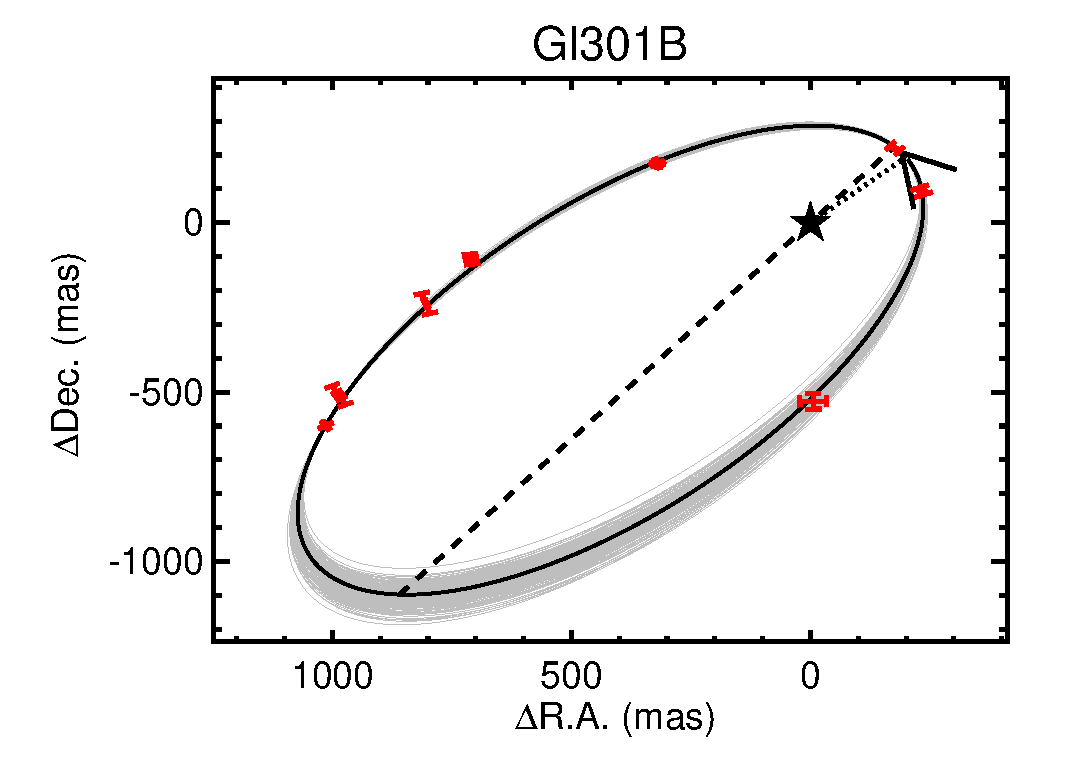
\includegraphics[width=0.32\textwidth]{Orbits/Gl301AB.eps}
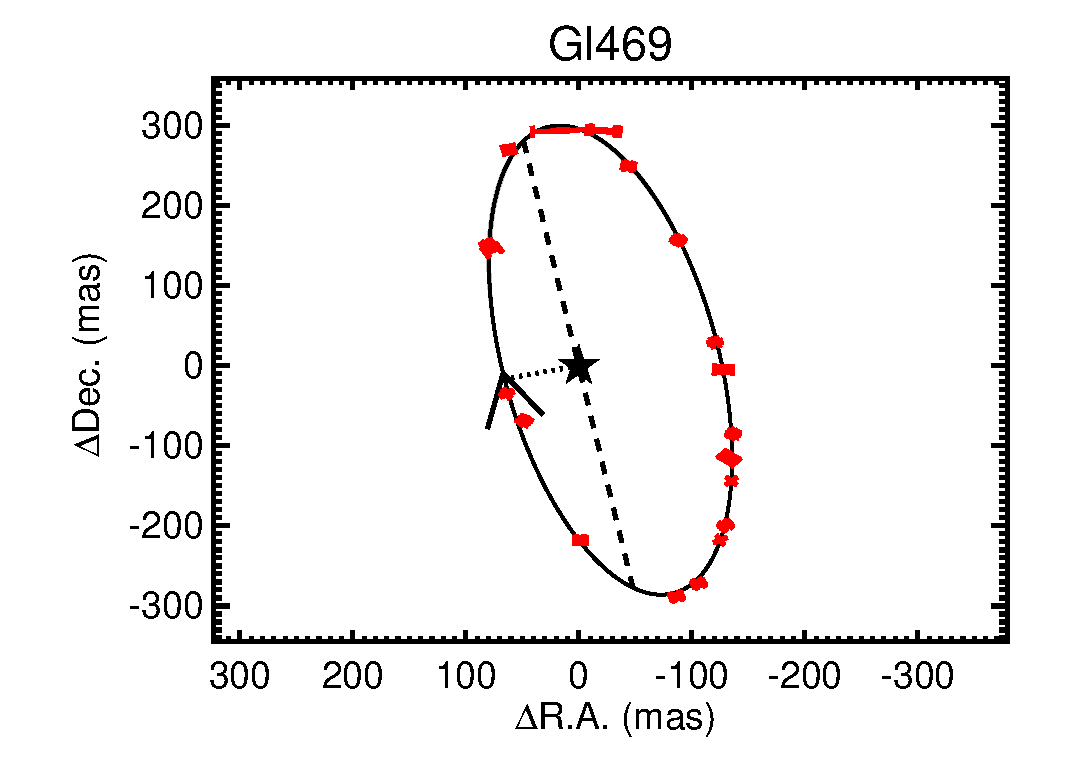
\includegraphics[width=0.32\textwidth]{Orbits/Gl469AB.eps}
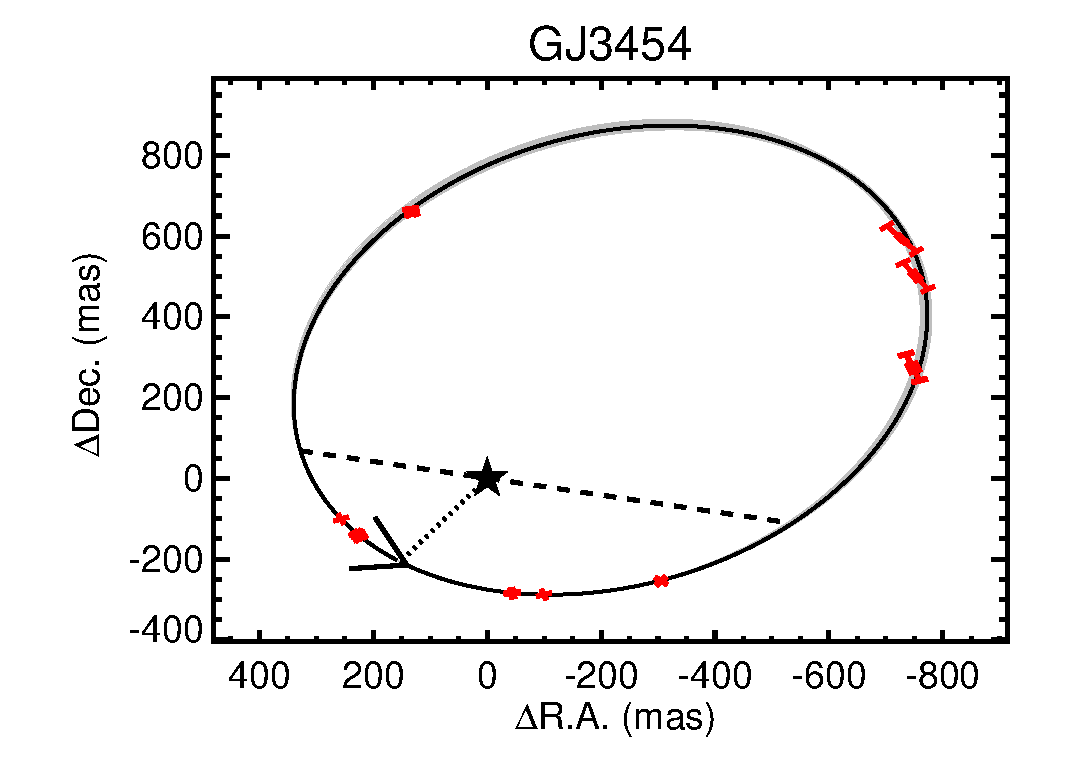
\includegraphics[width=0.32\textwidth]{Orbits/GJ3454AB.eps}
\caption{Example results of our orbit fitting procedure for Gl301AB (left), Gl469AB (middle), and GJ3454AB (right). Red points are individual measurements of the separation and position angle. Black solid line shows the best-fit (highest likelihood). Grey lines are drawn by randomly sampling 100 orbit fits from the MCMC fit to give an estimate of the errors. The dotted line marks the periastron passage, with an arrow for the orbital direction, and the dashed line indicates the line of nodes. For Gl301AB, there are no data for a large section of the orbit, but the final fit is relatively well constrained. For Gl469AB, high-quality astrometry is available for the full orbit, and the resulting errors on orbital parameters are so small that the grey lines cannot be seen. All other orbits are shown in Appendix~\ref{sec:a1}}
\label{fig:orbits}
\end{center}
\end{figure*}

Our orbital fits made heavy use of literature astrometry, many of which had no reported errors. Our method for assigning or correcting errors assumed that all measurements have a common missing error term per data source (Section~\ref{sec:litas}). It is more likely that errors depend on the separation and contrast ratio, as well as quantities that were not consistently reported, like weather, setup, and observational strategy. Further, this technique assumed an uncorrelated error term. In the case of an erroneous pixel scale or imperfectly aligned instrument, all measurements from a common instrument may be off in the same direction. In practice, it is difficult to correct for these effects without access to the raw data. The data suggests this does not impact our results; the final $\chi^2_\nu$ values for the best-fit orbits shows no correlation with the fraction of data from the literature versus our own measurements, and measurements taken on the same target and epoch but from different sources agree within errors. Further, many issues that might arise from a single source of data were mitigated by using a wide range of data sources, each of which were subject to different systematics. 

As an additional test, we tried refitting a subset of 10 randomly selected binaries twice, first doubling the error term added to the literature, then halving it. With the exception of one system that failed to converge with the doubled input errors, overall parameters and errors did not change significantly (although the final $\chi^2_\nu$ values changed). The main reason for this is that our measurements are generally far more more precise (with the exception of measurements from {\it HST}) and disproportionately weigh on the final solution. Further, in the case of significantly underestimated errors, the MCMC usually explores a range of solutions to result in a similarly broad posterior as the one derived using larger input errors. We conclude this treatment of errors does not significantly impact our final orbital fits. 

%Resulting fits all have $0.1<\chi^2_\nu<2$, within the expected distribution given the number measurements per orbit. This was in part a consequence of our method of assigning errors to literature data (Section~\ref{sec:litas}). However, we achieved reasonable $\chi^2_\nu$ values even when all or nearly all the data were from our own measurements, indicating that our astrometry measurements have reasonable assigned errors.

The nine systems from \citet{Dupuy2017} are labeled separately in Table~\ref{tab:sample}.

\section{Stellar Parameters}\label{sec:params}


\subsection{Parallaxes}\label{sec:plx}

Parallaxes for 54 of the targets were drawn from the literature. In general we adopted the most precise parallax available, although preference is given to parallaxes that accounted for the fact that the target is a binary and those with a baseline significantly different from the binary's orbital period. For $\simeq$1/3 of the sample, parallaxes were drawn from the new reduction of the Hipparcos data \citep{van-Leeuwen:2007yq}. A few systems are in hierarchical triples with a wider companion that also has an independent parallax measurement, which we used where possible. We drew parallaxes from \citet{Dupuy2017} along with their orbital solutions, and parallaxes from \citet{Benedict2016} for those overlapping with our own sample. Most of the remaining parallaxes were drawn from the general catalogue of trigonometric parallaxes \citep{van-Altena1995}.

Many of our targets do not have entries in the second data release of {\it Gaia} \citep[DR2, ][]{GaiaDr2,2018arXiv180409365G}. They were most likely excluded because centroid shifts due to orbital motion prevented a single-star solution (a requirement to be included in DR2). While many targets do have entries, we found significant differences between the {\it Gaia} values and earlier measurements \citep[including from {\it Gaia} DR1, ][]{gaiadr1}. This is most evident when we examine a few wide triples in {\it Gaia} DR2 (where the third star is several arc seconds away, and hence easily resolved); many such systems have significantly different parallaxes reported for the unresolved pair than for the wider companion. This strongly indicates that orbital motion on our targets is impacting the final parallax values or uncertainties even when a value is reported. We found no such issues with our other parallax sources, although some of this issue may be hidden by larger uncertainties.

We ultimately used {\it Gaia} DR2 parallaxes for only two systems, GJ1245AC and GJ277AC, where we adopted the parallax of the wider (resolved) B components. In both cases the B components are not known to harbor another unresolved star, and hence they should not be impacted by the same binarity issue. GJ 570BC, Gl 695BC, GJ 2005BC, and Gl 22AC also have wider companions. However, Gl 570A is extremely bright ($G\simeq5$) and hence may have an unreliable parallax, GJ 2005A has no entries in {\it Gaia} DR2, and the available parallaxes (from {\it HST} and Hipparcos) for Gl 695A,BC and Gl 22AC,B are more precise than the ones for Gl 695A and Gl 22B from {\it Gaia} DR2. 

For seven systems we derived new parallaxes using MEarth astrometry \citep{Nutzman:2008gf}. Updated parallaxes were measured following the procedure from \citet{2014ApJ...784..156D}. The only difference was we used a dataset with a baseline $\simeq$two years longer, which helps average out systematic errors arising from centroid motion due to the binary orbit, and significantly reduces the overall uncertainties. 

We list all parallaxes and references in Table~\ref{tab:sample}.

\subsection{\rm{[Fe/H]} }\label{sec:feh}

We estimated [Fe/H] using our SpeX spectra and the empirical relations from \citet{Mann2013a} for K5-M6 dwarfs, and \citet{Mann2014} for M6-M9 dwarfs. For the one target lacking a SpeX spectrum (Gl 54), we derive [Fe/H] using the optical calibration of \citet{Mann2013a} and a moderate-resolution optical spectrum taken from \citet{Gaidos2014}. These relations use a series of atomic lines (primarily Na, Ca, and K features) in the optical or NIR \citep[e.g.,][]{2010ApJ...720L.113R,Terrien:2012lr}, empirically calibrated using wide binaries containing a Sun-like primary and an M-dwarf companion \citep[e.g.,][]{2005A&A...442..635B,Johnson2009,Neves2012}. The calibrations were based on the assumption that components of such binaries have similar or identical metallicities \citep[e.g.,][]{2015ApJ...801L..10T}. Similar methods have been used extensively to assign metallicities across the M dwarf sequence \citep[e.g.,][]{Terrien2015,Muirhead2015,Dressing2017,2018ApJ...853...30V,2018ApJ...854..145M}. Final adopted [Fe/H] values are given in Table~\ref{tab:sample}. 

Uncertainties on [Fe/H] from such spectroscopic determinations are generally 0.08-0.12~dex. This exceeds the measurement uncertainties by a factor of 1.5-3 \citep{Newton:2014}. The difference may be due to inhomogeneities in the assigned primary stars' metallicities \citep[e.g.,][]{2015ApJ...805..126B,2016ApJS..225...32B,2016ApJS..226....4H}, as well as complications in using atomic lines as a proxy, which are not expected to scale perfectly with iron abundances \citep{Rojas-Ayala:2012uq,Veyette2016a}. The existing data suggest that relative abundances (one M dwarf relative to another) are far more precise than the overall scale (relative the Sun).% Based on the calibration samples in \citet{Mann2013a} and \citet{Mann2014}, we estimate the former to be reliable to $\simeq$0.05~dex, while the latter to $\simeq0.08$~dex. 

For all but two targets (Gl 65 and HD 239960), our NIR spectra are for the combined flux of the binary components. \citet{Mann2014} explored the issue of measuring metallicities of binaries with unresolved data by combining spectra of single-stars with similar metallicities and re-applying the same calibration. The bias introduced is negligible ($\lesssim0.02$~dex) when compared to overall uncertainties. The added scatter is smaller than the measurement uncertainties, and can be explained entirely by the Poisson noise introduced in the addition of component spectra. 

Three targets (LP415-20, 2M2140+16, and 2M2206-20) have SpeX spectra taken with a wider slit, yielding lower spectral resolution. The bands in \citet{Mann2014} are defined using a homogenous dataset taken with the narrow (0.3\arcsec) slit, so this difference may impact the derived [Fe/H]. We tested this by convolving a set of single-star SpeX spectra taken with the 0.3\arcsec\ slit with a Gaussian to put them at the appropriate lower resolution. The median of the derived [Fe/H] values changed by $<0.01$~dex, but the change varies between targets. Based on the resulting scatter, we estimate the errors on [Fe/H] from the lower-resolution spectra to be 0.12~dex on a Solar scale and 0.08~dex on a relative scale. These targets are marked separately in Table~\ref{tab:sample}. 

Two of the targets in our sample are L dwarfs (2M0746+20 and 2M1017+13). These both land above hydrogen burning limit, and hence are included in our analysis. However, the \citet{Mann2014} method contains no L dwarf calibrators. We report our derived [Fe/H] values for these systems, but advise treating the assigned values with skepticism until an L dwarf calibration becomes available. 

Two targets (HIP 95995 and HIP 96656) are too warm (earlier than K5) for the calibration of \citet{Mann2013a}. For these we take [Fe/H] values from \citet{2011A&A...530A.138C} and \citet{2010A&ARv..18...67T}, respectively. These [Fe/H] measurements are not necessarily on the same scale as those from \citet{Mann2013a}, which are calibrated against abundances of Sun-like stars from \citet{2015ApJ...805..126B,2016ApJS..225...32B}. Given reported variations in [Fe/H] for these stars, as well as [Fe/H] determination differences \citep{2014AJ....148...54H,2016ApJS..226....4H} we adopt conservative 0.08~dex uncertainties on both systems. 

\subsection{$K_S$-magnitudes} \label{sec:mags}

We initially adopted unresolved $K_S$ magnitudes from the Two Micron All Sky Survey \citep[2MASS,][]{Skrutskie2006}. For the brightest stars in our sample, some 2MASS magnitudes were saturated, and others may have systematically underestimated errors as they are near saturation. For these targets we recalculated $K_S$ magnitudes using available optical and NIR spectra, following the method of \citet{Mann2015a} and \citet{Mann2015b}. Optical spectra were taken from \citet{Gaidos2014}. Synthetic magnitudes were broadly consistent with 2MASS $K_S$ magnitudes (and at similar precision) for fainter targets ($K_S>7$). We only updated $K_S$ magnitudes for bright systems where where our synthetic photometry differed from the 2MASS value by more than 2$\sigma$ (five systems). We mark these systems in Table~\ref{tab:sample}. 

To compute $\Delta K_S$, we calculated the robust weighted mean of all contrast ratios derived from our AO data (Section~\ref{sec:astrometry}). For $\Delta K_S$, we used all data centered somewhere within the $K$ band (for astrometry we had no wavelength restriction). Errors on contrasts for a given epoch were based on the scatter in flux measurements between consecutive measurements. This may have underestimated errors arising from imperfect flat-fielding, uncorrected non-linearities in the detector, or wavelength-dependent flux losses from the optics or atmosphere, as well as intrinsic variability of the star. We compared $\Delta$m measurements of the same star using the same filter and instrument but on different nights (Figure~\ref{fig:magnitudes}). The comparison suggessted a missing error term of 0.017\,magnitudes. There were not enough data to test this for all filters and instruments, but we get a consistent value across all filters with sufficient data for a test, suggesting the problem is relatively independent of the filter used. We included this term as an additional error term in our computation of $\Delta K_S$.

\begin{figure}[htb]
\begin{center}
\includegraphics[width=0.47\textwidth]{errors.eps}
\caption{Distribution of contrast ratio differences (in units of standard deviations) for data taken on the same targets but in different nights. The red line is before adding a missing error term of 0.017 magnitudes, while the blue line shows the distribution after adding this. The grey dashed line shows the expected Normal distribution. The histograms are offset slightly for clarity, although identical bins are used as input.}
\label{fig:magnitudes}
\end{center}
\end{figure}

While all targets considered here had at least one measurement in a filter centered with the $K$ band, none of the filters used were an exact match for 2MASS $K_S$. Much of the data were taken with narrow-band $K_{\rm{continuum}}$ or Br$\gamma$ filters, for example. We transformed these into 2MASS magnitudes before computing final $\Delta K_S$. These corrections were usually small ($\lesssim0.1$ magnitudes), and details on their derivation are given in Appendix~\ref{sec:a1}.

\section{The Mass-Luminosity Relation}\label{sec:relation}

\subsection{Methodology}

For main-sequence stars, the mass-luminosity relation traditionally takes the form:
\begin{equation}\label{eqn:ml}
\frac{L_*}{L_\odot}  = C \left(\frac{M_*}{M_\odot}\right)^\alpha,
\end{equation}
where $\alpha$ depends on the dominant energy transport mechanism (e.g., radiative versus convective) and internal structure of the star \citep{2004sipp.book.....H}. This relation can depend significantly on chemical abundance and age, which produces a large scatter in the empirical mass-luminosity relation \citep[e.g.,][]{2010A&ARv..18...67T}. For M dwarfs on the main sequence, we can effectively ignore age, as they change negligibly on Gyr timescales \citep{BHAC15,MIST1}. We discuss issues of metallicity further in Section~\ref{sec:metal}.

It is convenient to write this in terms of \mks\ instead of $L_*$. Absolute magnitudes are more easily measured than overall luminosity, and this avoids introducing errors from uncertain bolometric corrections or the need to take flux-calibrated spectra in order to measure the bolometric flux directly. Switching to \mks\ also mitigates effects of metallicity, as the the $K$-band is heavily dominated by metal-insensitive CO and H$_2$O absorption bands. This has been seen both in stellar spectra \citep{Rojas-Ayala:2012uq} and model atmospheres (Figure~\ref{fig:metal}). The lower metallicity sensitivity of $K$-band is also a major reason \mks\ yields a tighter relation with $M_*$ and $R_*$ when compared to similar relations using an optical magnitudes \citep[e.g.,][]{Henry:1993fk,Delfosse2000,Mann2015b,Benedict2016}. 

\begin{figure*}[htp]
\begin{center}
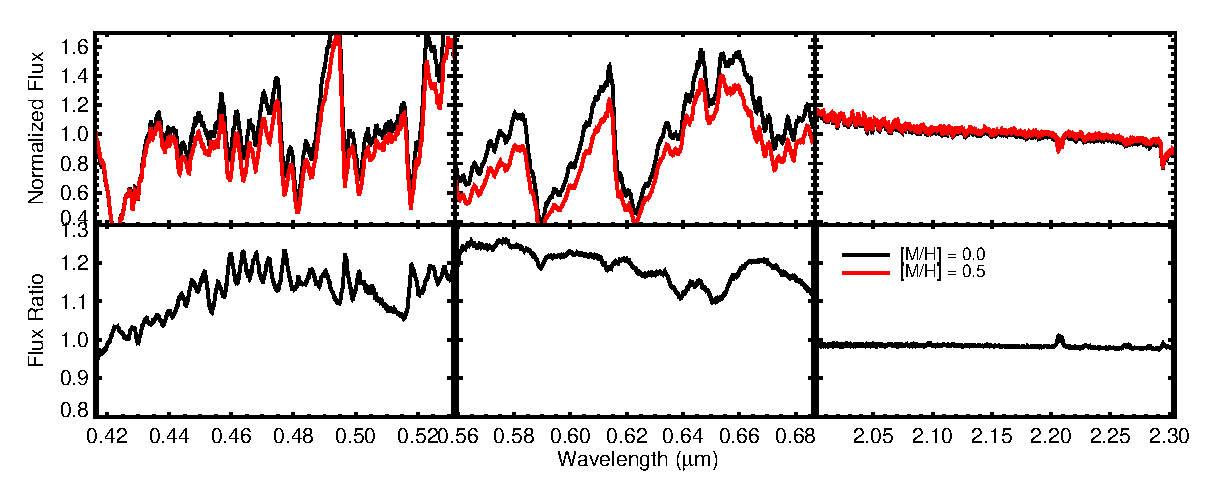
\includegraphics[width=\textwidth]{metallicity_effect.eps}
\caption{Effect of changes in [M/H] on a model spectrum at \teff=3200\,K, $\log(g)=5$ in $g$-band (left), $r$ (middle), and $K$ (right). The top panel shows [M/H]=0 (black) and [M/H]=+0.5 (red) spectra from the CFIST BT-SETTL models \citep{2012RSPTA.370.2765A}. The bottom panel shows the ratio of the two, highlighting how small an effect [M/H] has in the $K$-band compared to optical regions. The one feature that stands out in the $K$-band is the Na doublet, which is a commonly used as a metallicity diagnostic for dwarfs \citep{2010ApJ...720L.113R,Terrien:2012lr,Newton:2014}, and a gravity diagnostic for pre-main-sequence stars \citep[e.g.,][]{Schlieder2012}. }
\label{fig:metal}
\end{center}
\end{figure*}

Since absolute magnitudes are proportional to the log of the luminosity, we put Equation~\ref{eqn:ml} in terms of \mks\ and $\log(M_*/M_\odot)$. Our sample encompasses almost an order of magnitude in mass and hence a range of underlying stellar physics. No single $\alpha$ value is expected to fit over the full sequence. Instead, we assumed that $\alpha$ depends on \mks, which we approximated as a polynomial of the form:
\begin{equation}\label{eqn:mmk}
%\log \left( \frac{M_*}{M_\odot} \right) = a + b(M_{K_S}-zp) + c(M_{K_S}-zp)^2 + ...,%\mathscr{F}(M_{K_S}),
\log \left( \frac{M_*}{M_\odot} \right) = \sum_{i=0}^{n} a_i(M_{K_S}-zp)^i,
\end{equation}
where $a_i$, are the $n$ fit coefficients. The constant $zp$ is a zero-point (or anchor) magnitude, which we fixed at 7.5. This approximately corresponded to the logarithmic central mass of stars in our sample. Shifting $zp$ did not change the overall fit, but did make the shape more sensitive to small changes in the $a_i$ values. 

For the left hand side, we computed the total system mass ($M_{\rm{tot}}$) for each binary by combining the the orbital period ($P$) and angular semi-major axes ($a\arcsec$) from our fits to the orbital parameters (Section~\ref{sec:orbit}) with the parallaxes ($\pi$, Section~\ref{sec:plx}), following:
\begin{equation}\label{eqn:mass}
M_{\rm{tot}} = M_{1}+M_{2} = \frac{(a\arcsec/\pi)^3}{P^2},
\end{equation}
where $P$ is in years, $a\arcsec$ and $\pi$ are in arcseconds, and $M_{\rm{tot}}$ is in Solar masses. 

Because Equation~\ref{eqn:mass} does not provide component star masses, when fitting for the $a_i$ coefficients we performed the comparison between the predicted and dynamical {\it total} mass for each system. For this, we rewrote Equation~\ref{eqn:mmk} in terms of total mass:
\begin{eqnarray}\label{eqn:mmk2}
M_{tot} &=& 10^{b_1} + 10^{b_2},\\
b_j &=& \sum_{i=0}^{n} a_i(M_{K_S,j}-zp)^i, \label{eqn:mmk2_b}
\end{eqnarray}
where \mks$_1$ and \mks$_2$ are the primary and companion absolute $K$-band magnitudes, which were calculated from our measured $\Delta K_S$ and unresolved $K_S$ magnitudes (Section~\ref{sec:mags}). Equation~\ref{eqn:mmk2} could easily be modified for higher-order star systems, providing individual \mks\ magnitudes and the total mass of the system are known. %Additionally, in the case where the mass ratio is known for some systems (e.g., from radial velocities), we could trivially add this in as an additional constraint. 

We fit for the $a_i$ terms in Equation~\ref{eqn:mmk2} using the MCMC code \textit{emcee}, which lets us fit for the strong covariance between coefficients. Each coefficient evolved under uniform priors without limits, and was initialized to the best-fit value derived from \textit{MPFIT}. We ran the MCMC chain with 800 walkers for 750,000 steps after a burn-in of 50,000 steps. We tested values of $n$ (number of $a_i$ terms) from three to six. We found significant improvement in both $\chi^2$ and the Bayes factor for the best-fit relation using up to five constants, but both metrics gave negligible improvement when we move to a sixth. 

Errors on the dynamical mass are correlated to the errors on \mks. The system mass scales with $a^3$, which depends linearly with the parallax. As a result, the parallax was a major, if not the largest, source of uncertainty on the mass for most systems. Similarly, our $K_S$ magnitudes had relatively small errors (0.01-0.03\,mag), so \mks\ errors tended to be dominated by the parallax. Because this correlation is usually along (parallel to) the direction of the \mmk\ relation, it can improve the fit if properly taken into account (when compared to assuming uncorrelated errors). 

Our strategy was to treat distances of each system as a free parameter, letting them evolve under a strong prior from the observed parallax. The MCMC fit to Equation~\ref{eqn:mmk2} was provided $a\arcsec^3/P^2$ and $K_S$ (with uncertainties) for each system, from which total mass and \mks\ were recomputed from the varying parallax of each system at each step in the MCMC before making a comparison. Since the orbital information provides no constraint on the distance, this effectively forced the parallax to explore a distribution along the input prior. It is possible for the parallax posterior to shift off this prior if it provided better agreement with the relation as determined by the rest of the sample. However, in practice this does not happen; for all systems the parallax posterior matched the input values (Figure~\ref{fig:parallax}). 

\begin{figure*}[htb]
\begin{center}
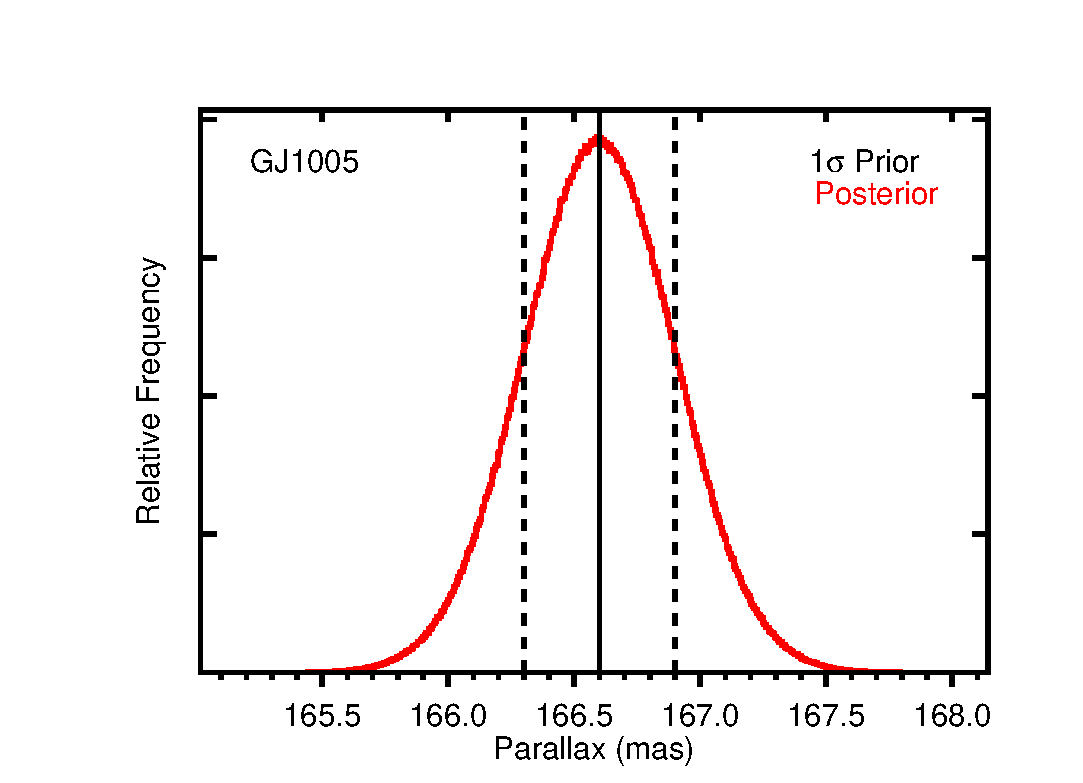
\includegraphics[width=0.32\textwidth]{plx_GJ1005.eps}
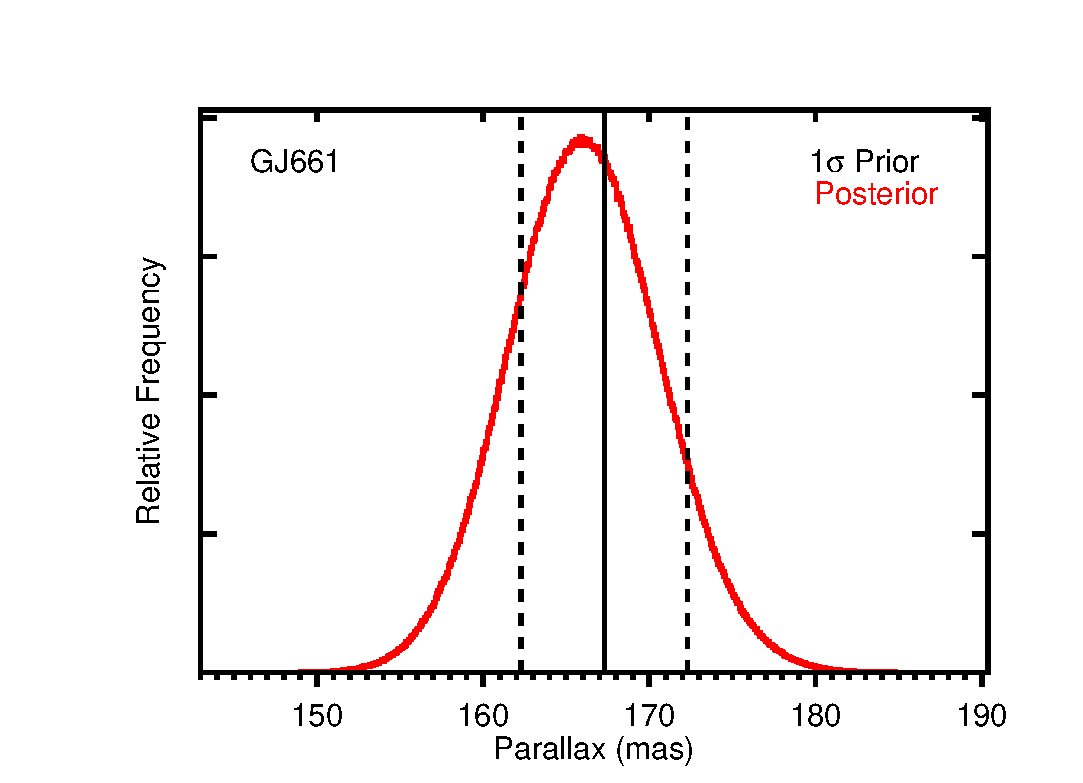
\includegraphics[width=0.32\textwidth]{plx_GJ661.eps}
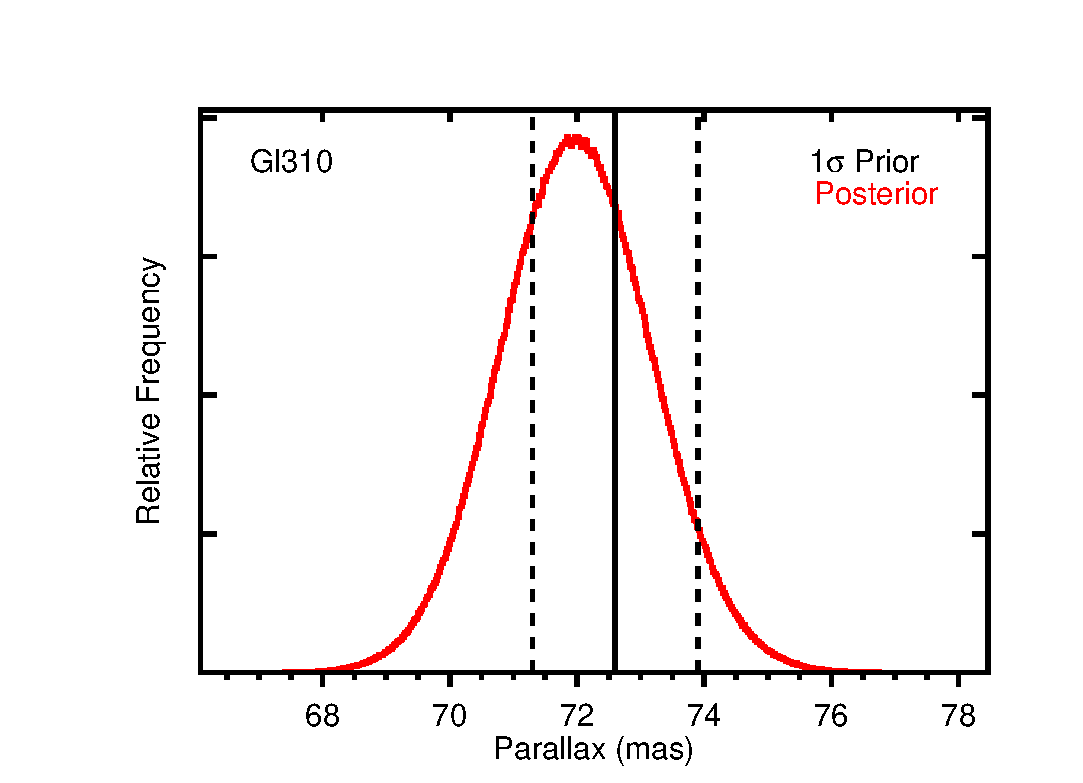
\includegraphics[width=0.32\textwidth]{plx_Gl310.eps}
\caption{A comparison of example input 1$\sigma$ priors (black lines) to the output posteriors (red distributions). Gl 310 represents one of the largest differences between the prior and posterior, highlighting that the measured parallax prior dominates the MCMC exploration. }
\label{fig:parallax}
\end{center}
\end{figure*}

For computational efficiency we assumed one-dimensional, Gaussian errors on $a\arcsec^3/P^2$, rather than including the orbital posteriors inside of our MCMC fit. Errors on $a\arcsec$ and $P$ from our orbits fits are correlated and sometimes non-Gaussian. However, the posteriors on $a\arcsec^3/P^2$ were described well by a Gaussian (Figure~\ref{fig:correlated}). The only deviations were the systems with the worst parameters overall, which tended to have somewhat asymmetric posteriors. However, these systems had little influence over the final fit.

\begin{figure}[htb]
\begin{center}
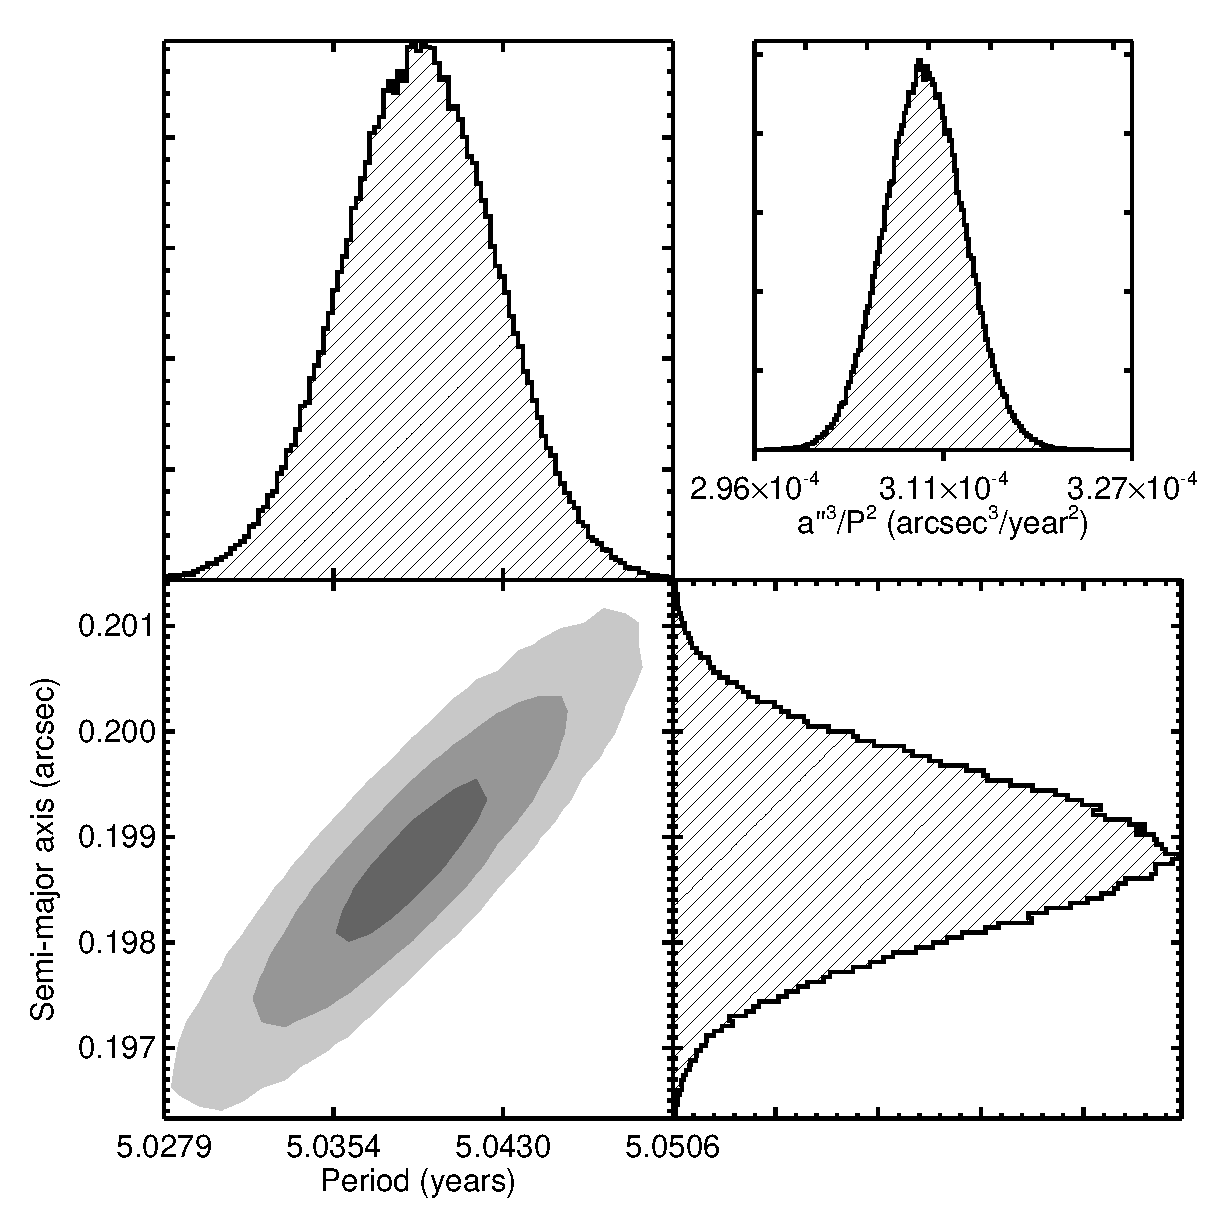
\includegraphics[width=0.47\textwidth]{LHS6167_corner.eps}
\caption{Example joint posterior on semi-major axis and orbital period (bottom left) for the system LHS 6167. Grey regions show 1, 2, and 3$\sigma$ (from darkest to lightest) of the points. The histograms above and to the right show the one-dimensional distributions of each parameter. The parameter fed into the \mmk\ fit is $a\arcsec^3/P^2$ (in arcsec$^3$ per year$^2$), which we show in the top right inset. }
\label{fig:correlated}
\end{center}
\end{figure}

For main-sequence dwarfs at fixed metallicity, more massive stars should always be brighter. To force this on our relation, we required that the resulting fit have a negative derivative (higher \mks\ always gives lower mass) over the full range of input objects considered. We tested running without this constraint, and found similar results over most of the parameter range considered. The major difference was near the edges of the relation. With this constraint the fit would sometimes become double valued (two \mks\ values that yield the same mass) at or just beyond the input sample.

\subsection{Results and Uncertainties}

We show the output coefficient posteriors in Figure~\ref{fig:fitpost}. The spread in the posteriors for individual coefficients is rather large, suggesting significant errors on each coefficient and a poor overall fit. However, the coefficients are also highly correlated. So for a given value assigned to four of the five fit coefficients, there is a relatively narrow set of solutions for the final constant. 



\begin{figure*}[p]
\begin{center}
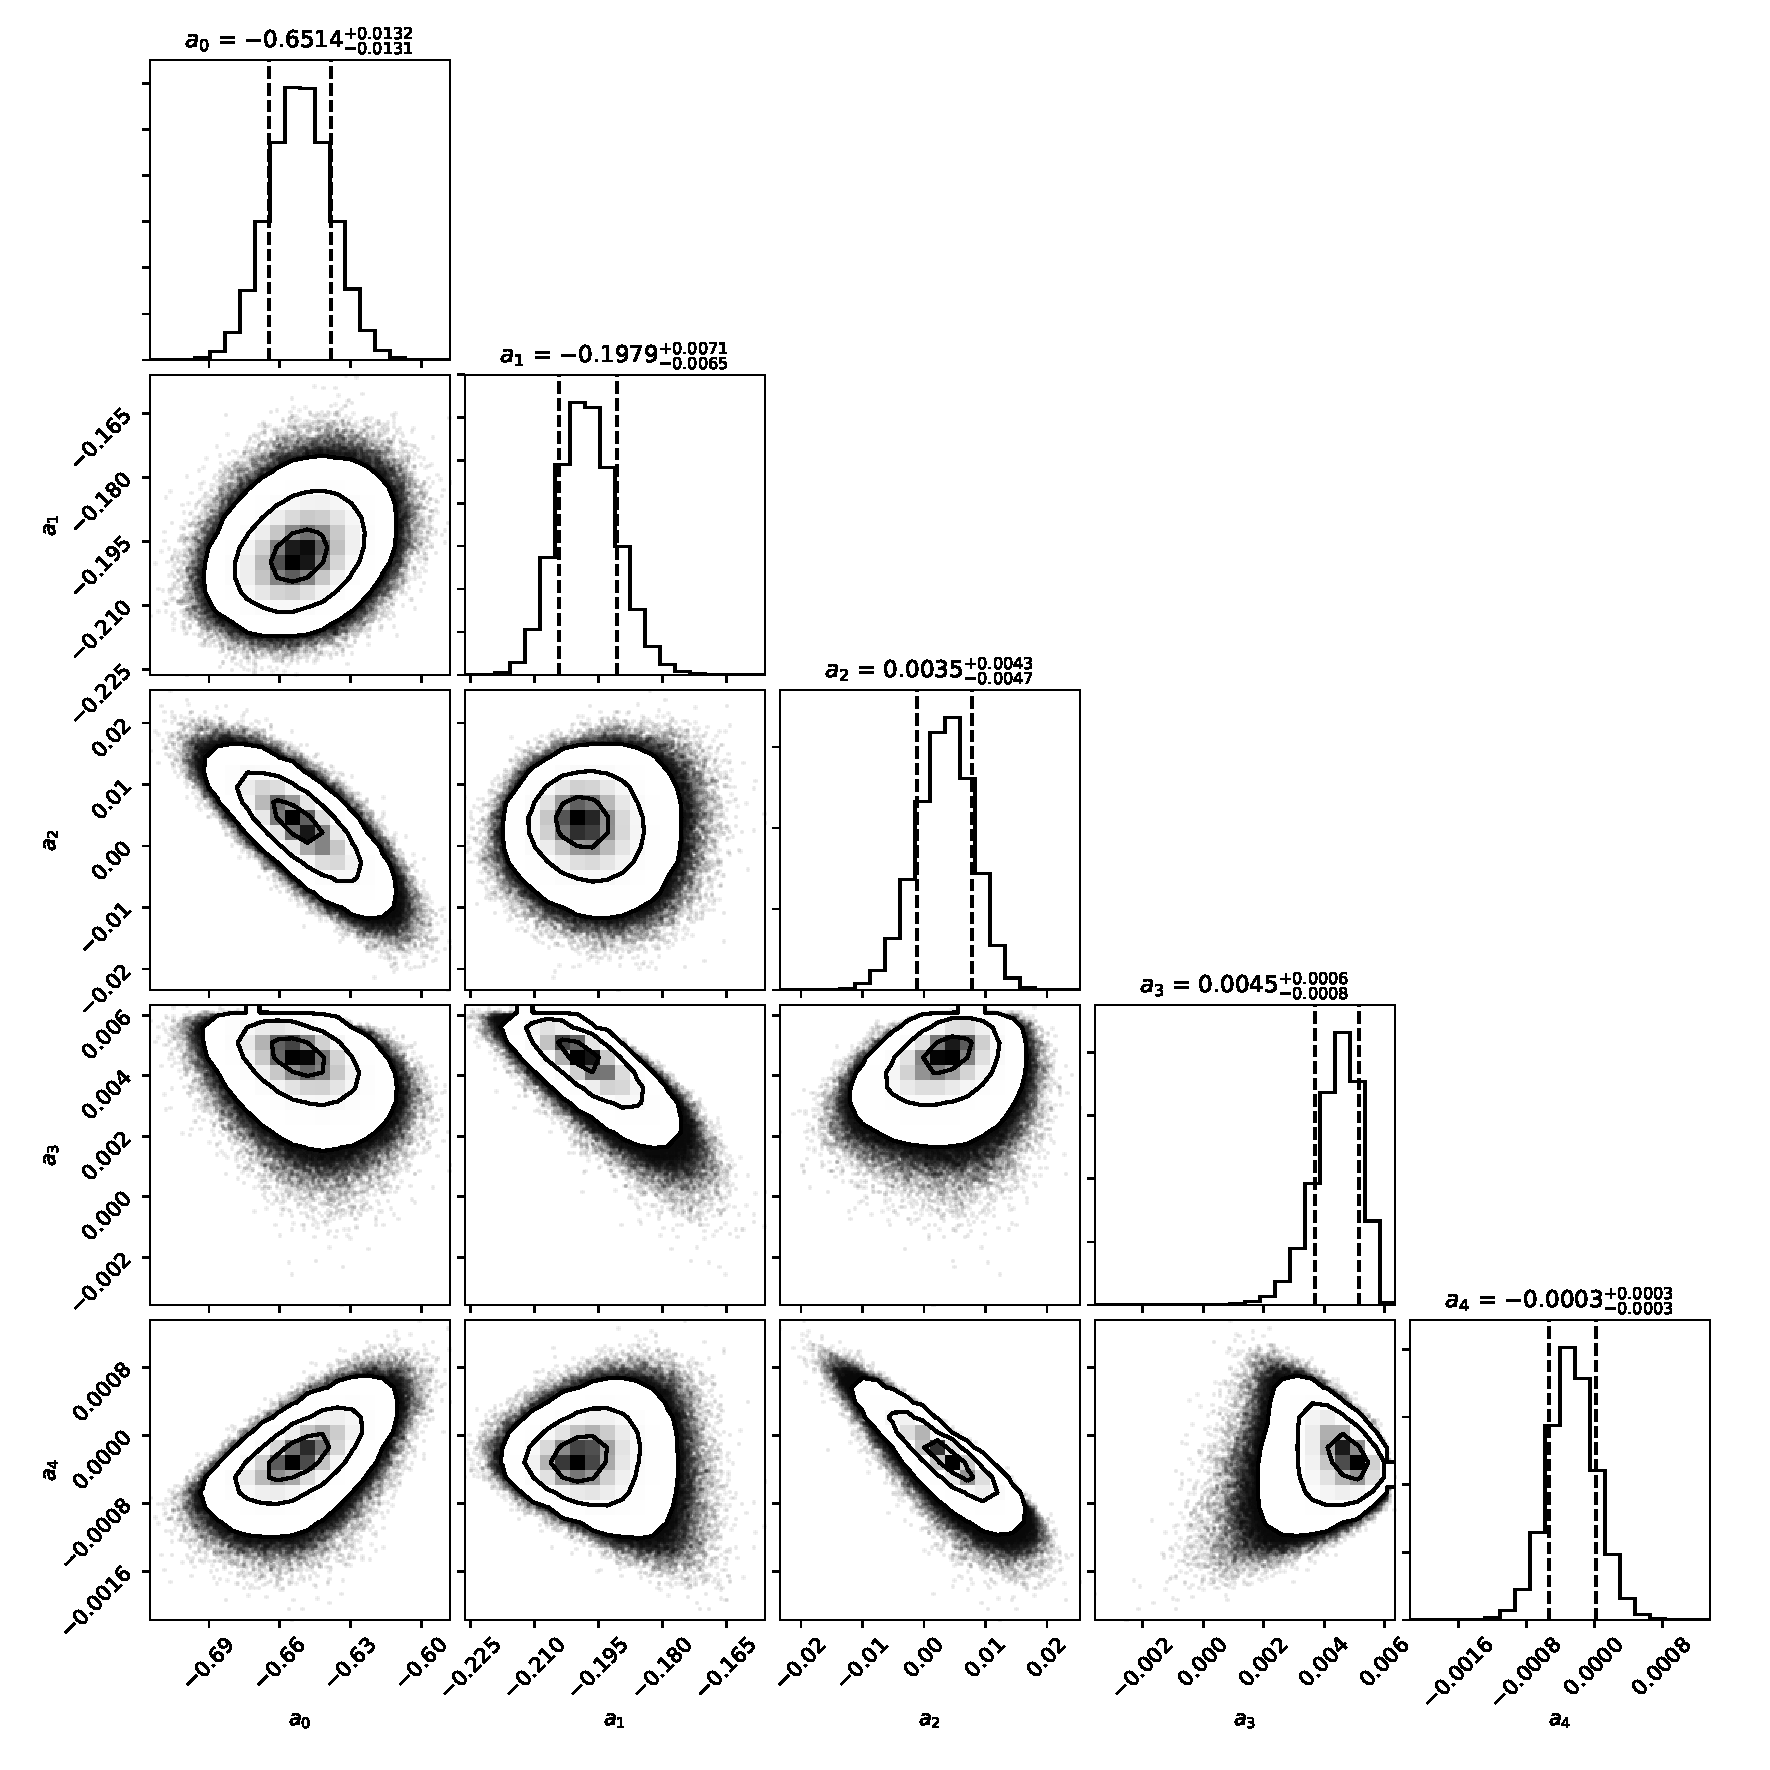
\includegraphics[width=0.9\textwidth]{output_params_5.pdf}
\caption{Posterior projections for the $a_i$ values derived from our MCMC fit to Equation~\ref{eqn:mmk2}. Contours denote the 1, 2, and 3$\sigma$ confidence intervals, and the dashed lines in the histogram mark 1$\sigma$.
Figure was generated using corner.py \citep{corner}.}
\label{fig:fitpost}
\end{center}
\end{figure*}

The final fit was tightly constrained over most of the sequence which we show in Figure~\ref{fig:relation} for individual masses, and combined masses in Figure~\ref{fig:m_m} (a more realistic representation of how the fit was done). We provide the best fit (highest likelihood) coefficient values in Table~\ref{tab:coeff}. Since the gain from four to five coefficients was small (but significant), we include coefficients for both in Table~\ref{tab:coeff}, but we adopt the five-parameter (4th order) solution for all analyses and figures.


\begin{figure*}[htp]
\begin{center}
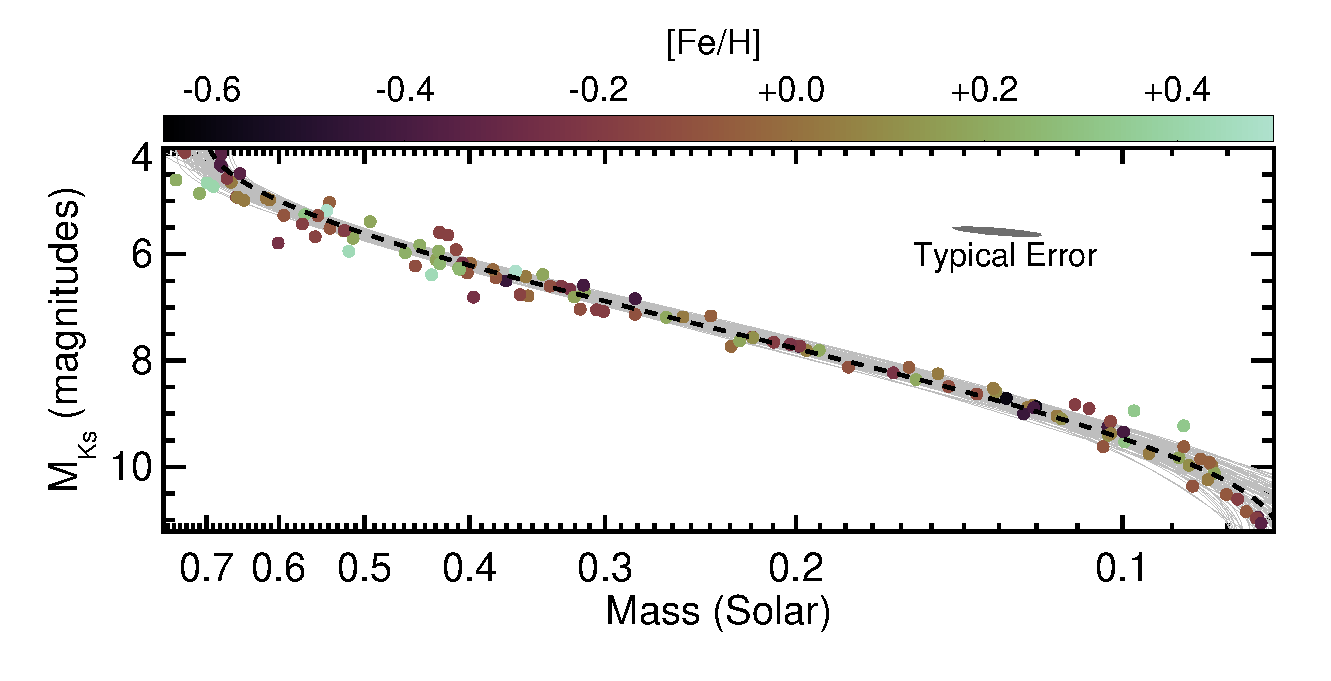
\includegraphics[width=\textwidth]{MK_mass_1.eps}
\caption{Absolute $K_S$-band magnitude as a function of mass for targets in our sample (circles). Points are color-coded by their estimated metallicity. We show a typical error ellipse in grey to highlight that errors on mass and \mks\ measurements are correlated, and usually parallel to the $M_*$-\mks\ relation (both depend on the parallax). The black dashed line indicates the best-fit (highest likelihood) from our MCMC analysis. To provide an estimate of the scatter in the relation as a function of mass, we show 100 randomly selected fits from the MCMC chain in grey. Note that our orbit fits only provide {\it total} mass; we used the mass ratios derived from the resulting \mmk\ relation for the purposes of this figure.  }
\label{fig:relation}
\end{center}
\end{figure*}


\begin{figure}[htp]
\begin{center}
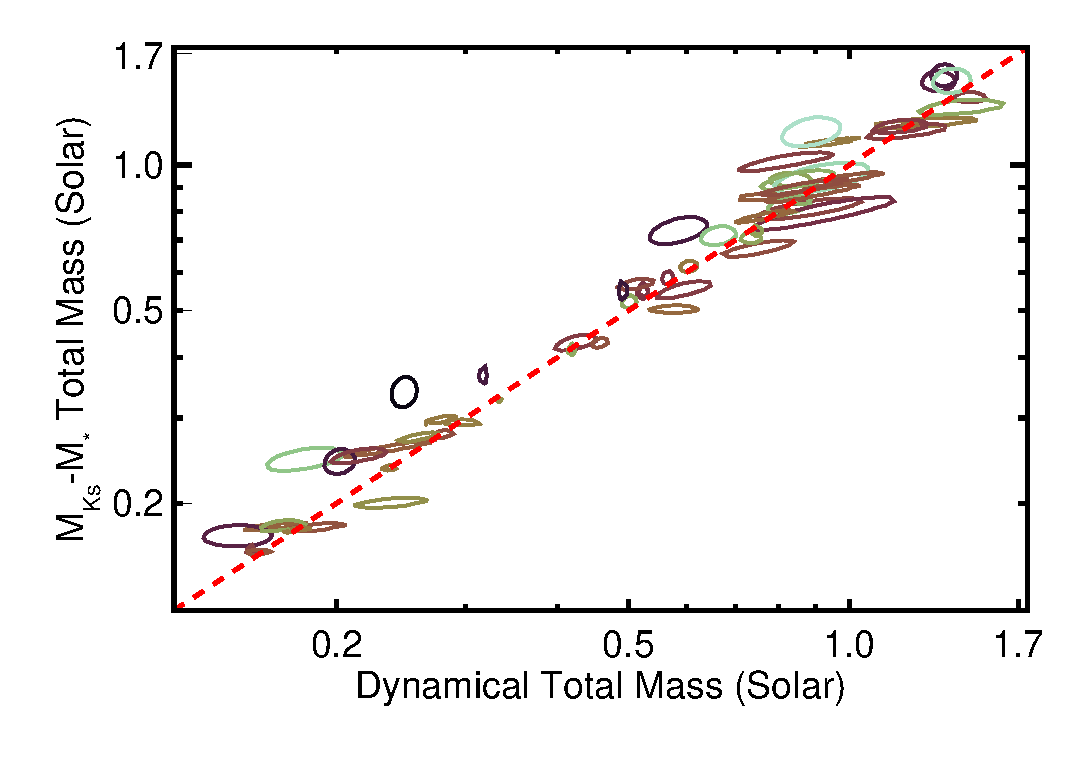
\includegraphics[width=0.47\textwidth]{Mass_mass_5_0.eps}
\caption{Predicted total (system) $M_*$ from the \mmk\ relation as a function of the total mass determined from the orbit fit. Ellipses represent $\simeq1\sigma$ distribution of values for each point, accounting for parallax errors common to both the predicted and dynamical mass. Color-coding by [Fe/H] matches that of Figure~\ref{fig:relation}.}
\label{fig:m_m}
\end{center}
\end{figure}


\begin{deluxetable*}{l l l l l l l }
\tablecaption{Best-fit Coefficients for Equations~\ref{eqn:mmk2} and \ref{eqn:mmk3}}
\tablehead{
\colhead{$a_0$} & \colhead{$a_1$} & \colhead{$a_2$} & \colhead{$a_3$} & \colhead{$a_4$} & \colhead{f} & $\chi^2_\nu$ 
}
\startdata
 -0.663193 &  -0.203256 &  8.202319$\times10^{-3}$ &  5.389355$\times10^{-3}$ & -5.489318$\times10^{-4}$& \nodata & 1.46 \\
-0.642761 &  -0.201882 & -7.462048$\times10^{-4}$ &  4.741565$\times10^{-3}$ & \nodata &   0.058 &  1.58 \\
\hline
-0.649004 &  -0.201198 &  1.770185$\times10^{-4}$ &  4.701115$\times10^{-3}$ & \nodata &\nodata & 1.96 \\
 -0.641361 &  -0.205263 &  3.107211$\times10^{-3}$ &  5.301090$\times10^{-3}$ & -2.199428$\times10^{-4}$ &  0.068 & 1.42  \\
\enddata
\label{tab:coeff}
\tablecomments{The first row is the preferred fit, as the $f$ parameter is currently considered not significant. If [Fe/H] is considered the second row is preferred over the last.}
\end{deluxetable*}

To estimate the uncertainty the relation we computed the standard deviation in the derived masses for a fixed \mks\ across all MCMC steps, which we report in Table~\ref{tab:err}. In the best-constrained regions ($5\lesssim$\mks$\lesssim7$, $0.3\lesssim M_*\lesssim0.6$) the relation is good to 2-3\%. However, the fit is significantly less-well constrained near the edges, where mass errors are 7-8\%. Some of this is due to expected behavior of polynomials near the edge and a lack of data on the extreme ends. Stars at the high-mass end of our sample also have weaker orbital constraints overall.

\begin{deluxetable}{l l l l l l l }
\tablecaption{Error in \mmk\ Relation}
\tablehead{
    \colhead{$M_{K_S}$} & \colhead{$M_*$} & \colhead{$\sigma_{M_*}^a$} & \colhead{$\sigma_{M_*}^a$} & \colhead{SpT$^b$} \\
    \colhead{(mag)} & \colhead{$M_\odot$} & \colhead{$M_\odot$} & \colhead{\%} & 
}
\startdata
\multicolumn{5}{c}{No [Fe/H] term, 5 $a_i$ terms}  \\
\hline
 4.0 & 0.712 & 0.024 & 0.034 & K4.5 \\
 4.5 & 0.679 & 0.015 & 0.022 & K6.5 \\
 5.0 & 0.611 & 0.013 & 0.021 & M0.0 \\
 5.5 & 0.524 & 0.011 & 0.020 & M1.5 \\
 6.0 & 0.434 & 0.009 & 0.020 & M2.5 \\
 6.5 & 0.352 & 0.008 & 0.023 & M3.0 \\
 7.0 & 0.281 & 0.008 & 0.028 & M3.5 \\
 8.0 & 0.179 & 0.006 & 0.032 & M4.5 \\
 8.5 & 0.144 & 0.005 & 0.032 & M5.0 \\
 9.0 & 0.118 & 0.004 & 0.033 & M6.0 \\
 9.5 & 0.100 & 0.004 & 0.038 & M6.5 \\
10.0 & 0.086 & 0.004 & 0.047 & M7.5 \\
10.5 & 0.077 & 0.005 & 0.060 & M9.0 \\
11.0 & 0.071 & 0.006 & 0.080 & L1.0 \\
\hline
\multicolumn{5}{c}{[Fe/H] term, 4 $a_i$ terms}   \\
\hline
 4.0 & 0.731 & 0.028 & 0.038 & K4.5 \\
 4.5 & 0.679 & 0.015 & 0.023 & K6.5 \\
 5.0 & 0.605 & 0.011 & 0.018 & M0.0 \\
 5.5 & 0.519 & 0.010 & 0.020 & M1.5 \\
 6.0 & 0.434 & 0.009 & 0.021 & M2.5 \\
 6.5 & 0.354 & 0.008 & 0.022 & M3.0 \\
 7.0 & 0.285 & 0.006 & 0.022 & M3.5 \\
 8.0 & 0.182 & 0.004 & 0.025 & M4.5 \\
 8.5 & 0.147 & 0.004 & 0.028 & M5.0 \\
 9.0 & 0.120 & 0.004 & 0.033 & M6.0 \\
 9.5 & 0.100 & 0.004 & 0.038 & M6.5 \\
10.0 & 0.086 & 0.004 & 0.044 & M7.5 \\
10.5 & 0.076 & 0.004 & 0.054 & M9.0 \\
11.0 & 0.071 & 0.005 & 0.068 & L1.0 \\
\enddata
\label{tab:err}
\tablecomments{This table assumes \mks\ (and [Fe/H]) are known perfectly. Total errors on $M_*$ should take into account errors in the measured parameters and the relation. }
\tablenotetext{$a$}{The uncertainty in the resulting $M_*$ at a given $M_{K_S}$}
\tablenotetext{$b$}{Spectral types are given for reference, but are extremely rough because of a significant dependence on metallicity. It is not recommended to use this table as a means to compute \mks\ or $M_*$ from a spectral type. }
\end{deluxetable}

The values in Table~\ref{tab:err} can be used as an approximate reference for estimating errors on the output mass for a given \mks\ if combined with errors from the distance and $K_S$ magnitude. However, this can be misleading, as the posterior is not Gaussian or symmetric over much of the mass range. It is better to sample the posterior at a given \mks\ to produce a posterior in mass. To facilitate use of our \mmk\ and help provide realistic uncertainties, we include the fit posteriors and provide a simple code that provides output $M_*$ posteriors\footnote{\href{https://github.com/awmann/M_-M_K-}{https://github.com/awmann/M\_-M\_K-}} given an \mks\ and error. 

The fit with the highest likelihood yields a $\chi^2_\nu$ of 1.5 with 57 degrees of freedom (accounting for correlated errors). The larger than expected scatter is primarily driven by a handful of systems that agree with the best-fit to within $\simeq$3\%, but also have small total mass uncertainties ($\lesssim$1\%). The MCMC explores the range of solutions, so if we factor in the scatter in the final \mmk\ relation then the $\chi^2_\nu$ value decreases to 0.98. As a result, using the fit posteriors provides uncertainties on $M_*$ that encompass the larger scatter. 

The larger than expected scatter could be due to systematically underestimated uncertainties, most likely in the input distances. As we noted with the {\it Gaia} DR2 parallaxes (Section~\ref{sec:plx}), orbital motion can shift the centroid and hence impact the measured parallax. This is particularly true for systems with orbital periods near an alias of one year (the parallax signal's period). Most of the systems included were not impacted by this because they either had have their parallaxes drawn from a nearby bound (and single) star, were calculated accounting for the presence of the binary, or have orbits far from the timescale of the parallactic signal. But a small impact on the sample could explain the higher scatter. 

If the parallactic or orbital errors were underestimated this could bias our result towards the most precise points. We explored this possibility by redoing our MCMC analysis adding a free parameter that uniformly increases the parallax uncertainty of all systems. The final fit parameters and resulting relation were negligibly different from those derived without the added error term, and the only meaningful change was a reduction in the $\chi^2_\nu$ of the best-fit solution. Because the change was small, we did not explore adding more sophisticated error terms to the adopted parallax, such as using the orbital fits to model the deviation in the unresolved binary centroid. 

Another possibility for this scatter is stellar physics not well accounted for in Equation~\ref{eqn:mmk2}, such as metallicity. %We investigate this in the next Section.

\subsection{The role of metallicity}\label{sec:metal}

We explored the expected effects of [Fe/H] on the \mmk\ relation using the Mesa Isochrones and Stellar Tracks \citep[MIST,][]{MIST0,MIST1}. We also tested the Dartmouth Stellar Evolution Database \citep[DSEP,][]{Dotter2008}, and found results to be broadly in agreement. We prefered MIST because their model atmospheres include a newer set of molecular lines (e.g., TiO) that are important in M dwarfs and may impact the synthetic photometry. The Lyon models \citep[BHAC15,][]{BHAC15} use a wrapper atmosphere in reasonable agreement with nearby stars with interferometrically determined \teff\ values \citep{Boyajian2012,Mann2013c}, and go to lower masses than DSEP and MIST. However, the BHAC15 models cover only solar metallicity. 

We show the expected \mks\ tracks from MIST for different metallicities in Figure~\ref{fig:mk_metal} alongside our empirical determinations. MIST models do not extend below 0.1$M_\odot$, so we restricted our comparison to above that mass. For this comparison we assumed a fixed age of 5\,Gyr, although the choice of age from 1-10\,Gyr makes a negligible difference for the mass range shown. Note that metal-rich stars are expected to be {\it less luminous} in \mks\ (and $L_{\rm{bol}}$) for a fixed $M_*$, whereas the opposite trend is seen for a fixed \teff\ and most color selections. 

\begin{figure}[htp]
\begin{center}
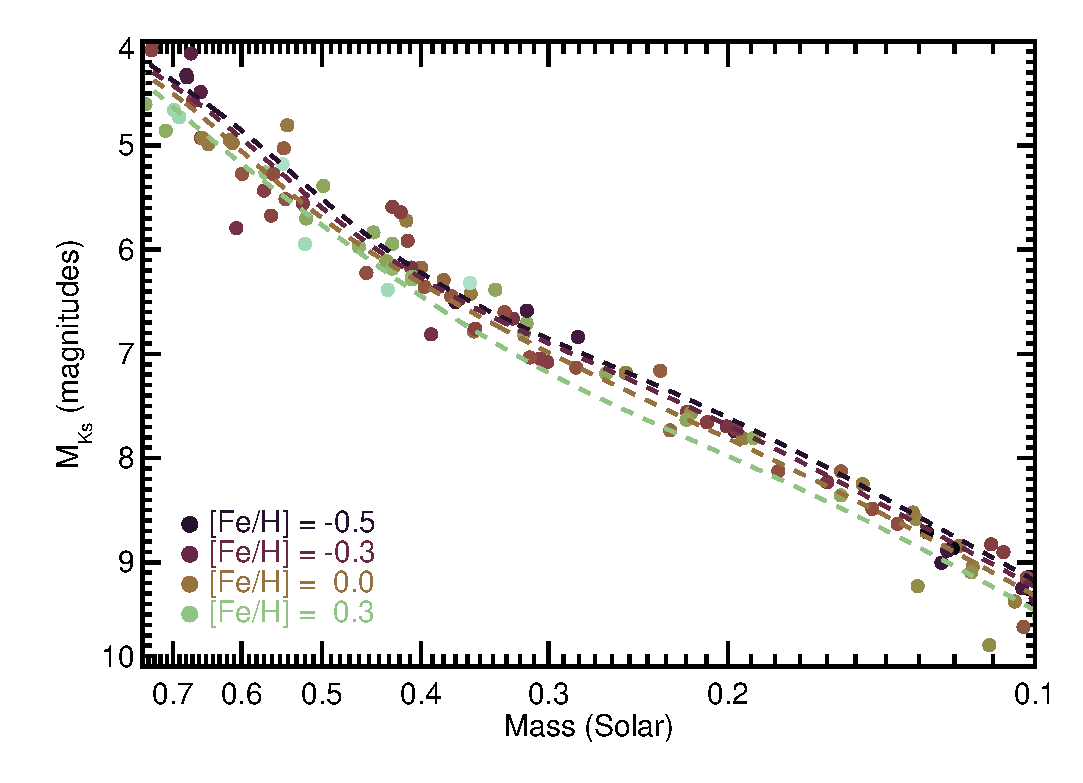
\includegraphics[width=0.47\textwidth]{Model_metal_0.eps}
\caption{\mks\ as a function of $M_*$ using MIST tracks of different metallicities (dashed lines) compared to empirical mass determinations (points). Color-coding by metallicity is the same for the points and lines, and matches the color scale of Figure~\ref{fig:relation}. The plot cuts at 0.1$M_\odot$, as the MIST models do not go below this limit. }
\label{fig:mk_metal}
\end{center}
\end{figure}

Above 0.4$M_\odot$ there is a slight trend for metal-rich stars in our sample to land below the median sequence, as expected from the models. However, many metal-poor stars also land below the sequence, and there is no obvious trend below 0.4$M_\odot$. We made this comparison more quantitative by interpolating over the model grid to create a predicted mass for each system using \mks\ and [Fe/H]. The predicted system masses were statistically worse than those from our best-fit relation ($\chi^2_\nu$ of 6.5 using the model grid versus 1.5 with Equation~\ref{eqn:mmk2}), and worse than simply assuming every star has [Fe/H]=-0.3 or [Fe/H]=0.0 ($\chi^2_\nu$ of 3.9 and 4.1). Allowing a zero-point correction to all metallicities (i.e., assuming they are systematically off from the model scale) improves the result ($\chi^2_\nu=4.0$), but a metallicity-free solution is still preferred. This strongly suggests that the models are overestimating the effect of [Fe/H].

The residuals from our best-fit relation confirmed a weak (or no) effect on the derived $M_*$ due to changes in [Fe/H], as we show in Figure~\ref{fig:metal_resid}. A Spearman rank test yielded no significant correlation between the residuals and [Fe/H]. We tried resampling the measurements using their uncertainties, and $<$1\% of samples showed a significant correlation. We also repeated this test, but restricted to just the best-characterized systems ($<5\%$ precision on mass) and still found no significant trend with [Fe/H]. 

\begin{figure}[htp]
\begin{center}
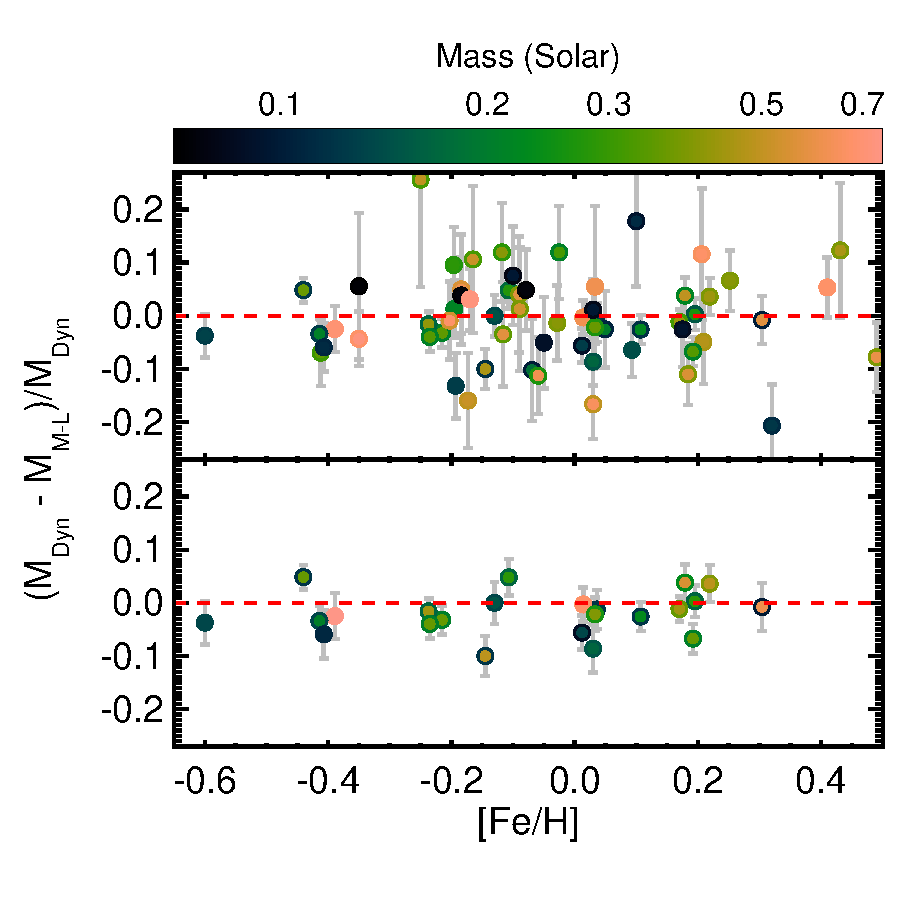
\includegraphics[width=0.47\textwidth]{residual_metal5.eps}
\caption{Fractional difference between the orbital and predicted system mass as a function of metallicity of the system. The top panel contains all systems, while the bottom shows just those with $<$5\% uncertainties on $M_*$. Points are color-coded by the masses of components, with the inner dot corresponding to the primary star's estimated mass, and the outer circle the companion's estimated mass. }%Quoted errors in mass account for the scatter in the \mmk\ relation.} 
\label{fig:metal_resid}
\end{center}
\end{figure}

Our sample is limited in its [Fe/H] range; 64\% of the targets are $-0.2<$[Fe/H]$<+0.2$ and only one target has [Fe/H]$<-0.5$. It is possible that our best-fit relation masked any [Fe/H] term by shifting the fit to match the typical metallicity of stars at a given \mks. We explored this by fitting for a term in [Fe/H] of the form:
\begin{eqnarray}\label{eqn:mmk3}
M_{tot} &=& (1+f[\rm{Fe/H]})\left(10^{b_1} + 10^{b_2}\right),
\end{eqnarray}
where $b_j$ is defined in Equation~\ref{eqn:mmk2_b}. This form assumes that a linear change in [Fe/H] corresponds to a fractional change in $M_*$ (e.g., f=0.1 would correspond to a 10\% change in derived $M_*$ per dex for a fixed \mks). This is generally consistent with the evolutionary models, although there is a change in the scale ($f$) over the range of masses considered here. 

For this analysis we excluded the two L dwarfs from the sample because of questionable assigned metallicities. As with our fit to Equation~\ref{eqn:mmk2}, we tested range of values for $n$ (number of $a_i$ coefficients). When including the [Fe/H] term, we found significant improvements in the fit up to $n=4$, compared to $n=5$ without $f$. Our MCMC fitting method was otherwise identical to that outlined in Section~\ref{sec:relation}. Since we were primarily interested in the {\it relative} effect of [Fe/H], and not necessarily the absolute scale, we assumed the smaller (relative) errors on [Fe/H] (see Section~\ref{sec:feh}).

We show the output coefficient posteriors in Figure~\ref{fig:fitpost_feh} and list the best-fit coefficients in Table~\ref{tab:coeff} for both the third- ($n=4$) and fourth-order ($n=5$) fits. Although the best-fit value of $f$ is relatively small ($\simeq$0.06 per dex [Fe/H]), the spread is rather broad ($\pm$0.06 per dex), a consequence of the narrow range of [Fe/H] values compared to overall measurement uncertainties. 

\begin{figure*}[p]
\begin{center}
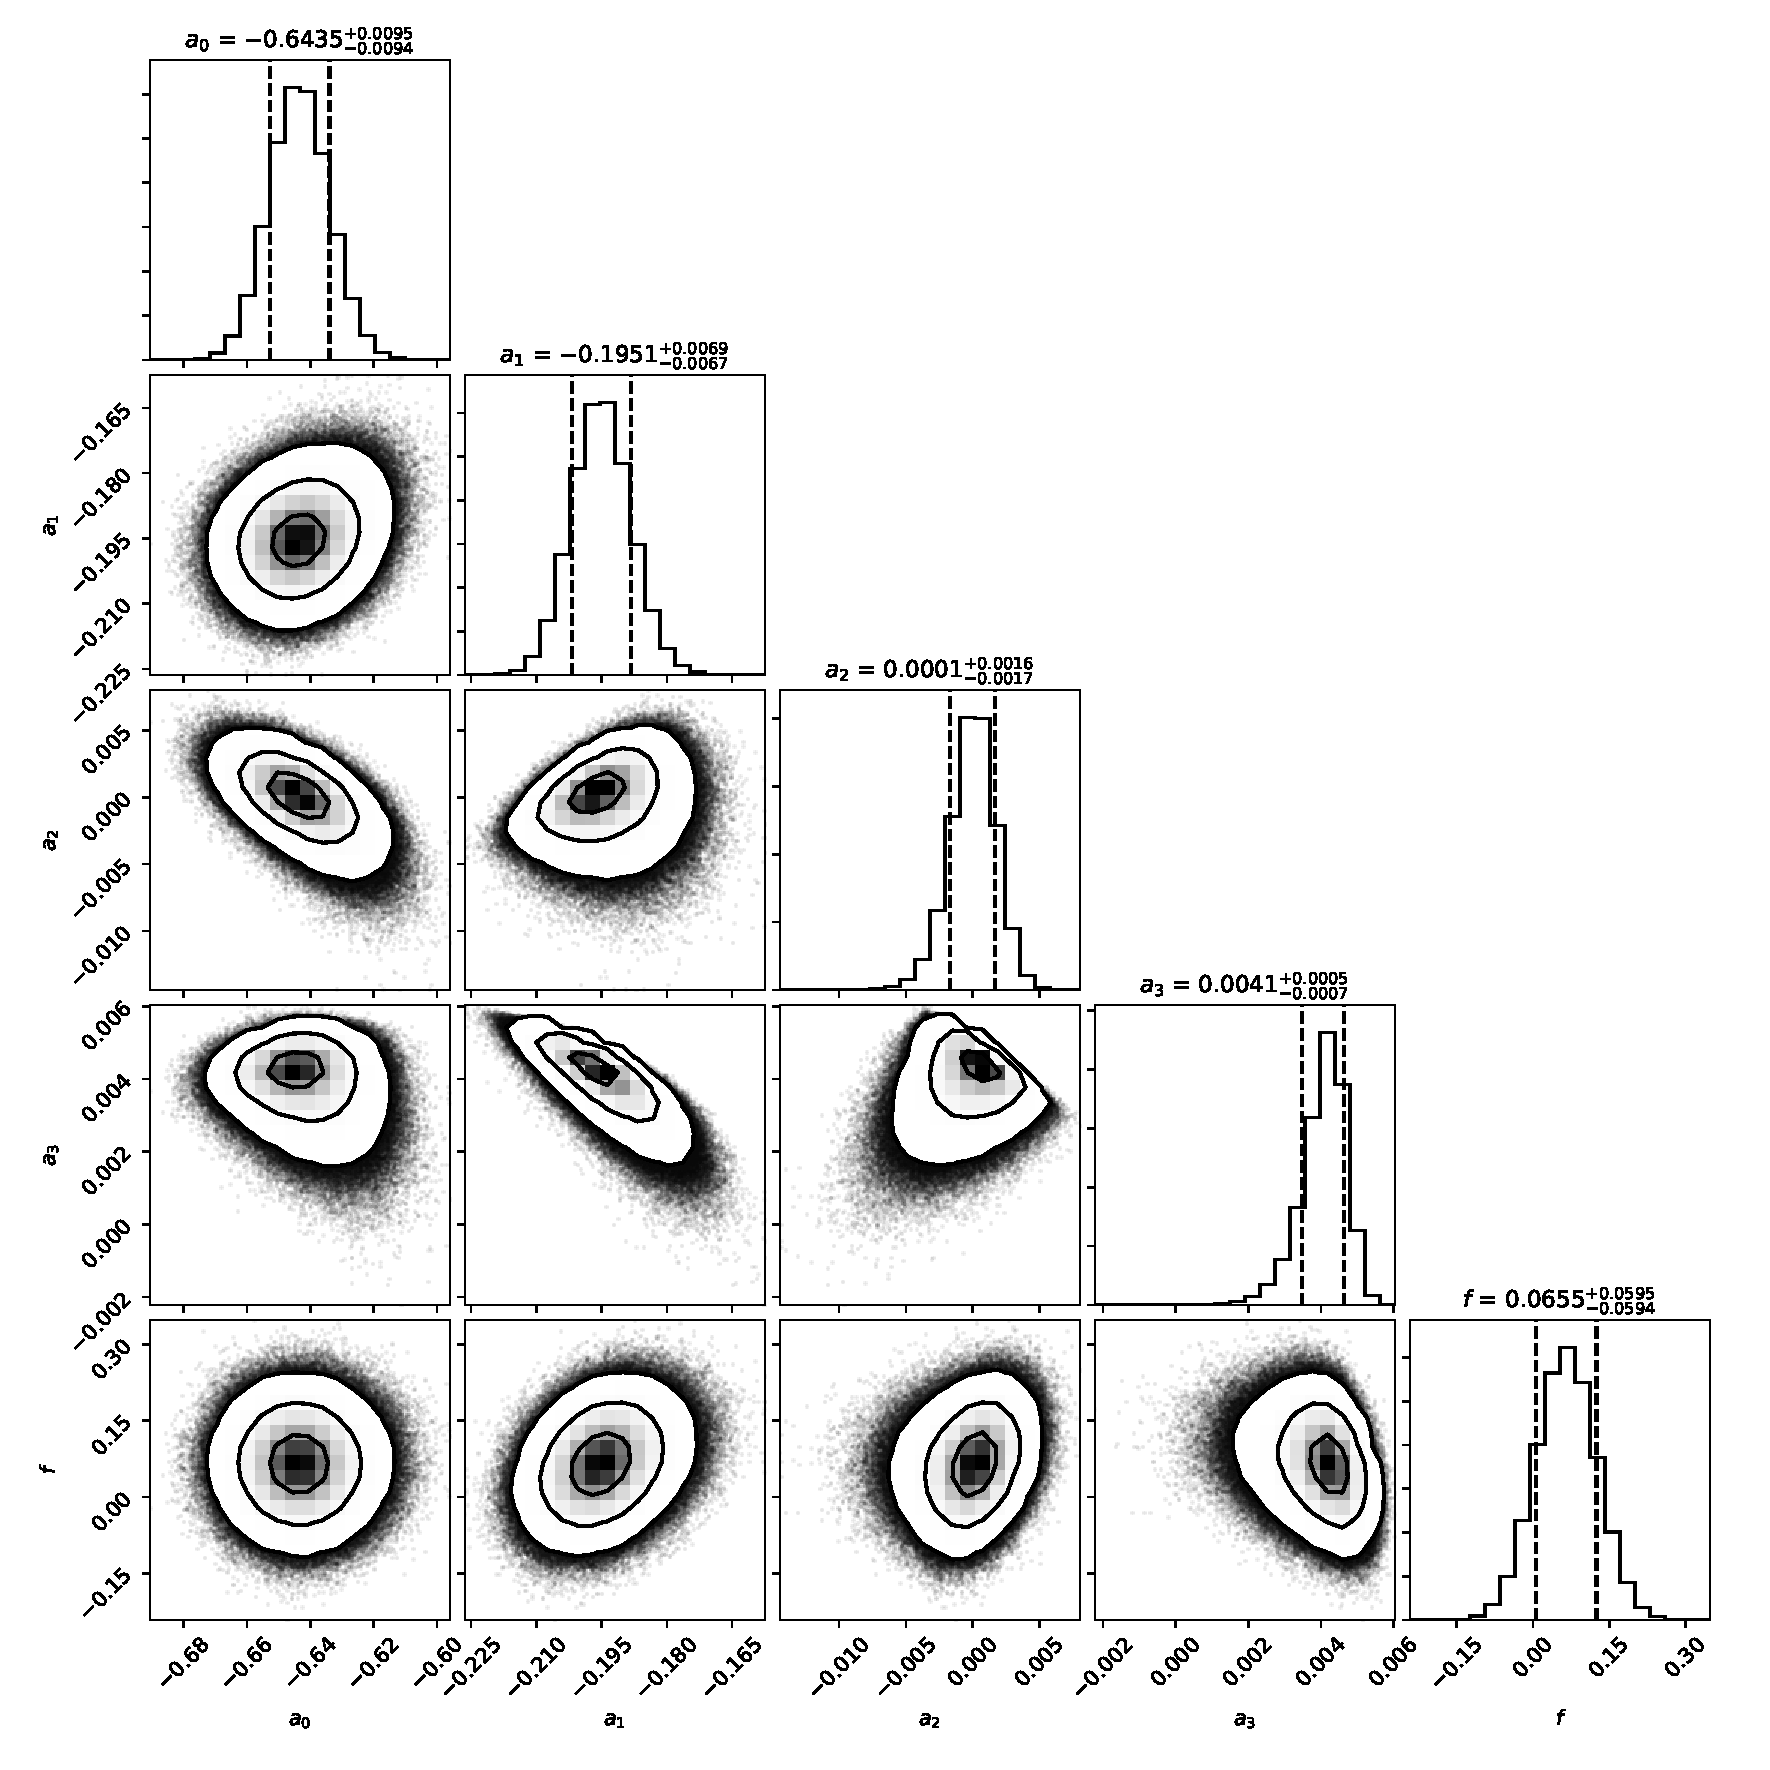
\includegraphics[width=0.97\textwidth]{output_params_4feh.pdf}
\caption{Same as Figure~\ref{fig:fitpost}, but for the fit following Equation~\ref{eqn:mmk3}, i.e., including the [Fe/H] term, $f$. }
\label{fig:fitpost_feh}
\end{center}
\end{figure*}


To compare to the models, we fit the MIST grid points in the same manner as the empirical dataset following Equation~\ref{eqn:mmk3}. In Figure~\ref{fig:f} we show the posterior on $f$ from the model grid compared to that from the dynamical masses. While the posteriors have some overlap, more than 96\% of the difference between the two posteriors ($f_{\rm{model}}-f_{\rm{dynamical}}$) is $>0$, indicating (with marginal significance) that the models overpredict the effect of [Fe/H] on the \mmk\ relation. It is unclear if (if true) this applies to the full mass range considered; there is some indication that the metallicity effect is stronger for higher-mass stars in the sample. The models suggest $f$ is $\simeq$30\% larger for [Fe/H]$<-1.0$. Thus a set of subdwarf binaries will provide more leverage to test over what mass range, if any, the discrepancy with the models is statistically significant. 

\begin{figure}[htp]
\begin{center}
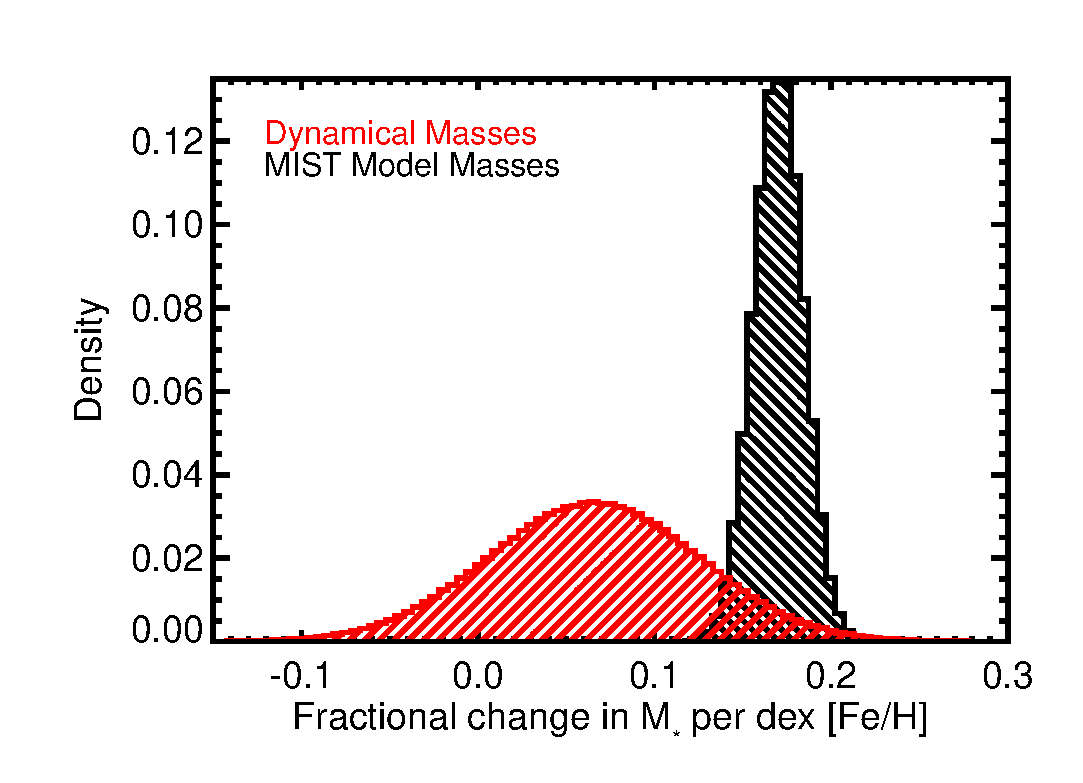
\includegraphics[width=0.47\textwidth]{F_plot.eps}
\caption{Comparison of the posterior on $f$ (fractional change in $M_*$ per dex in metallicity for a fixed \mks; Equation~\ref{eqn:mmk3}) predicted by the MIST models (black) compared to that using our dynamical masses (red). There are an identical number of points in each posterior and the bin sizes are the same. }
\label{fig:f}
\end{center}
\end{figure}


\subsection{Comparison to previous relations}\label{sec:other}

\subsubsection{\citet{Delfosse2000}}

\citet{Delfosse2000} provided one of the most commonly used \mmk\ relations, covering $0.1M_\odot<M_*0.6M_\odot$. Like our work, the calibration was build primarily on astrometric binaries. Nearly all the targets in \citet{Delfosse2000} were included in our sample, with the exception of triple systems and eclipsing binaries, both of which we intentionally avoided because of the complexity of computing total masses in the first scenario and estimating \mks\ in the latter. Because of the sample overlap, consistency is expected. However, a comparison can be useful to see how past use of \citet{Delfosse2000} may change with our more precise results.

We show the comparison in Figure~\ref{fig:delfosse}, including the points used in the \citet{Delfosse2000} calibration as well as the two fit lines. The relations are in agreement to better than 10\% over the full mass range considered, and within 5\% over most of the calibration region ($0.15M_\odot \lesssim M_* \lesssim 0.5M_\odot$). Given errors often quoted for the \citet{Delfosse2000} relation (5-10\%) the relations are consistent within errors. However, the relation presented here is a factor of 2-3 more precise over the whole mass regime. 

\begin{figure}[htb]
\begin{center}
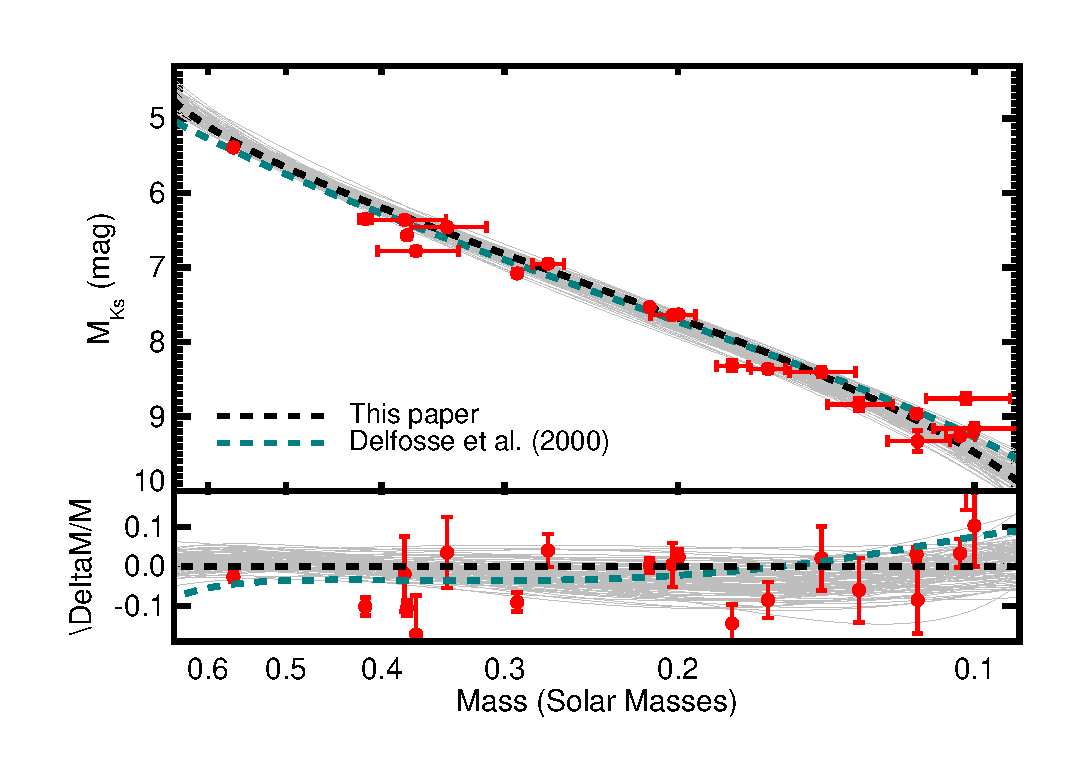
\includegraphics[width=0.47\textwidth]{Delfosse_comp.eps}
\caption{Absolute $K_S$-band magnitude as a function of mass for astrometric binaries analyzed by \citet{Delfosse2000} (red circles). The resulting $M_*$-\mks\ relation from \citet{Delfosse2000} is shown as a teal dashed line, while the best-fit relation from this paper is shown as a blacked dashed line (with error in grey as in Figure~\ref{fig:relation}). The bottom panel shows the residual of the \citet{Delfosse2000} points compared to our relation, with the \citet{Benedict2016} relation in teal for reference. Errors in the residuals only reflect errors in the mass and \mks, and do not account for errors in our $M_*$-\mks\ relation. }
\label{fig:delfosse}
\end{center}
\end{figure}

\subsubsection{\citet{Mann2015b}}

\citet{Mann2015b} built a catalog of 183 M dwarfs with precise \teff\ and $R_*$, calibrated against radii measurements from long-baseline optical interferometry \citep{Boyajian2012} and precision bolometric fluxes \citep[e.g.,][]{Mann2015a,2015MNRAS.447..846B}. Masses were measured for these stars by interpolating the parameters onto an updated version of the DSEP models as described in \citet{Feiden2013,Feiden2014} and \citet{Muirhead2014}. Although these masses were model-dependent, when combined with the more empirical radii, they precise reproduced the mass-radius relation from low-mass eclipsing binaries. The consistency between these relations and the empirical determinations from eclipsing binaries suggested that the model-based masses were accurate to $\simeq$3\% or better, and motivated the development of a \mmk\ relation from the \citet{Mann2015b}. sample. A comparison to our relation can be seen in part as a test on the updated DSEP models, in addition to the results given in \citet{Mann2015b}. 

We show our fit with uncertainties alongside \citet{Mann2015b}'s in Figure~\ref{fig:mann}. The two fits track each other extremely well, with a maximum divergence of $\simeq$5\%. Given the quoted 2-3\% uncertainties from \citet{Mann2015b} and the 2-3\% scatter in our relation, this difference is not significant. There is a hint of tension at the high-mass end, where our MCMC posterior is asymmetric, and at 0.2-0.3$M_\odot$ where the difference is the largest, but never does the the offset exceed the estimated uncertainties. 

\begin{figure}[htb]
\begin{center}
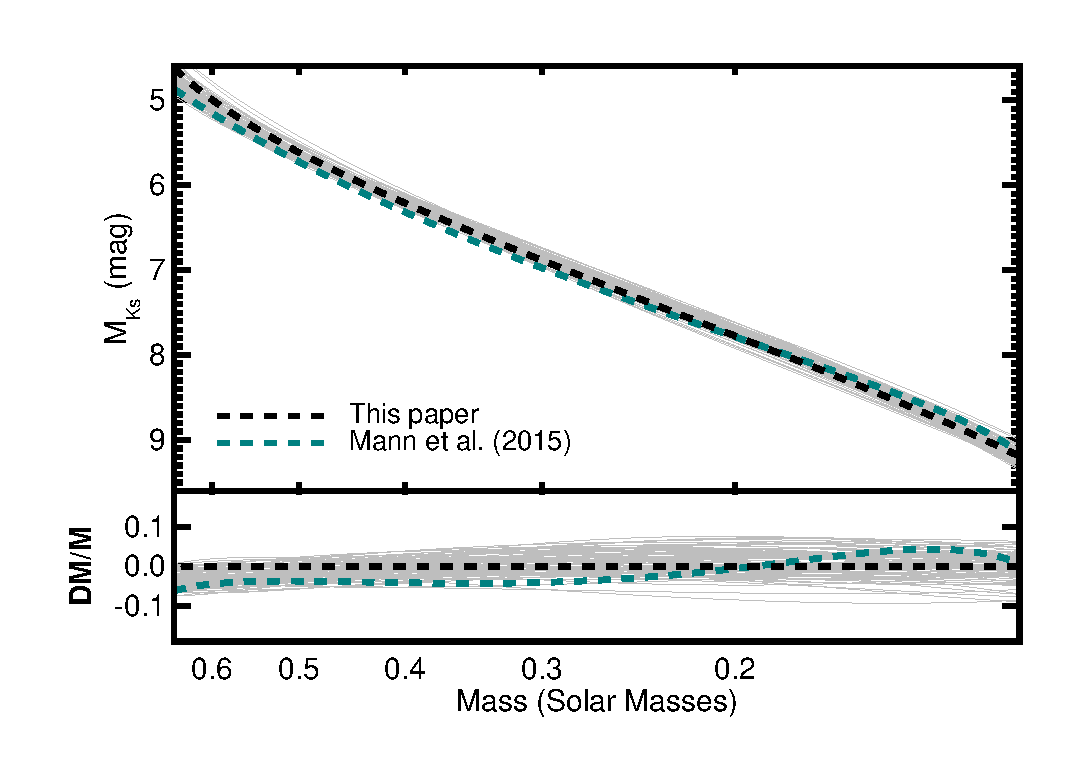
\includegraphics[width=0.47\textwidth]{Mann_comp.eps}
\caption{Comparison of $M_*$-\mks\ from \citet{Mann2015b}, shown as a teal dashed line, to that from this paper, which is shown in black, with 100 randomly selected realizations of the MCMC (as with Figures \ref{fig:relation} and \ref{fig:delfosse}). Residual is shown in the bottom panel. Individual points from \citet{Mann2015b} on which the calibration is based are not shown (for clarity), but they follow a tight sequence around the teal line. Only the range of masses covered by \citet{Mann2015b} are shown. }
\label{fig:mann}
\end{center}
\end{figure}




\subsubsection{\citet{Benedict2016}}
Like our work, the \citet{Benedict2016} relation was also based primarily on masses derived from M dwarf astrometric binaries. The \citet{Benedict2016} uses absolute astrometry from {\it HST} fine guidance sensors and radial velocities for a subset of systems. In addition to the exquisite precision provided by {\it HST}, this combination yields individual masses, and independent constraints on the systems parallax. So although our sample is larger and contains most of the targets in \citet{Benedict2016}, their analysis is not subject to many of the complications of our own. Differences between the two results could therefore shed light on complications with our use of total masses and perhaps reveal complications with our input parallaxes.

We compare our \mmk\ relation \citet{Benedict2016}'s in Figure~\ref{fig:benedict}. The two relations are in excellent agreement for $0.09M_\odot\lesssim M_* \lesssim 0.25M_\odot$. Below this regime, the \citet{Benedict2016} fit is anchored by the one star, GJ1245C. They have only two other stars in this low-mass regime (GJ 2005B and C), which had large errors when compared to rest of their sample. GJ1245AC is in our sample, but we use a parallax from \citet{GaiaDr2} on GJ 1245B for this system, which places it $5.5\sigma$ more distant that the parallax adopted by \citet{Benedict2016}. Our parallax-free orbital parameters for this system are in excellent agreement with \citet{Benedict2016}, but the \citet{GaiaDr2} parallax makes the final parameters more consistent with our overall relation. Since the \citet{Benedict2016} parallax accounted for the binarity of this system, the origin of difference between these two parallaxes unclear. If GJ 1245B is itself an unresolved binary, this could explain the discrepant parallax. If the \citet{Benedict2016} parallax is correct, we also need to explain why GJ 1245C is significantly more luminous than similar-mass stars.

%It is possible that GJ1245 is young, which would help explain its luminosity. GJ1245ABC (B is $\simeq$7\arcsec\ away) all have sub-day rotation periods and show significant flaring \citep{2015ApJ...800...95L,2017ApJ...834...85N}. Late-M dwarfs lose their initial rotation slowly, so such short rotation periods and flare rates are not uncommon at this mass \citep{Newton2016,2018arXiv180307708P}. We can only conclude that GJ1245 is likely $<2$\,Gyr, which cannot necessarily explain its luminosity. Further, GJ1245A ($M_*=0.117M_\odot$, \mks=8.890) lands slightly {\it below} our relation, showing no evidence of overluminosity. The system would need to land in a narrow range of ages where A is solidly on the main-sequence, but C is still contracting \citep[$\simeq$400-600\,Myr based on Lyon models, ][]{BHAC15}. 

 Above 0.3$M_\odot$, \citet{Benedict2016} yields masses as much as 10\% higher than our own for a fixed \mks. Our fit agrees reasonably well with the binaries analyzed by \citet{Benedict2016} in this mass regime. The divergence is driven by points not analyzed by \citet{Benedict2016}, but included in their fit from earlier literature sources. 


\begin{figure}[htb]
\begin{center}
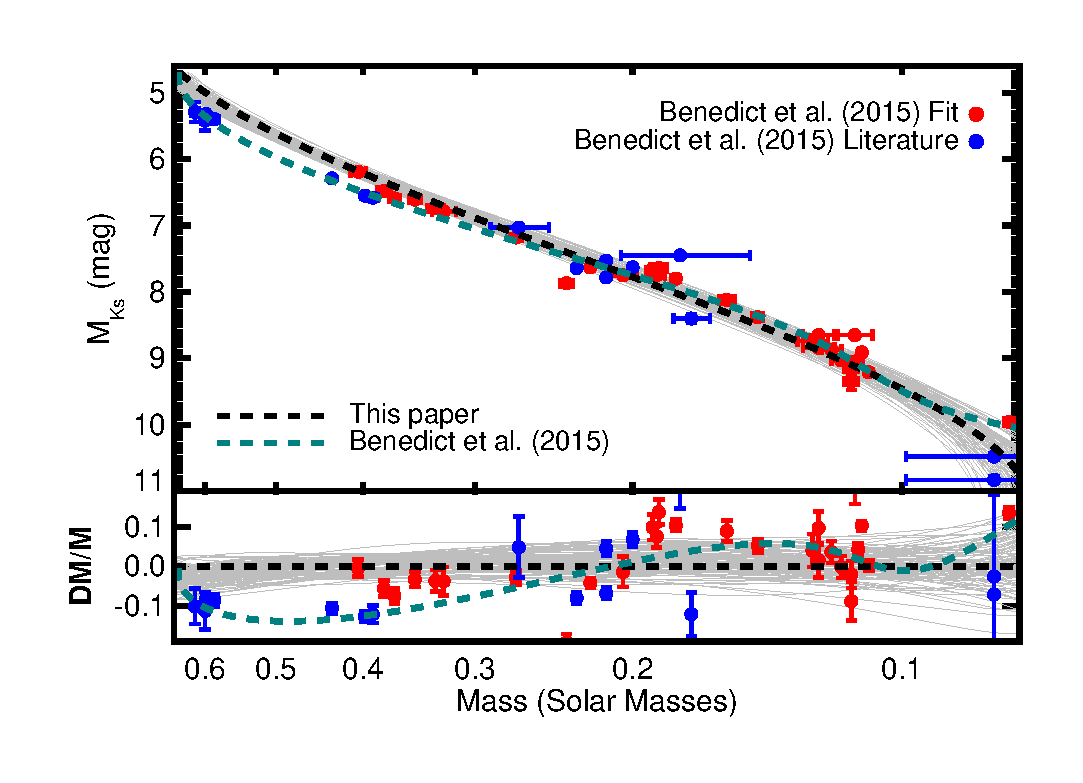
\includegraphics[width=0.47\textwidth]{Benedict_comp.eps}
\caption{Absolute $K_S$-band magnitude as a function of $M_*$ for astrometric binaries analyzed by \citet{Benedict2016} (red circles) and those used in the \citet{Benedict2016} relation, but pulled from the literature (blue circles). The resulting $M_*$-\mks\ relation from \citet{Benedict2016} is shown as a teal dashed line, while the best-fit relation from this paper is as a blacked dashed line (with random samplings in grey as in earlier figures). The bottom panel shows the residual of the \citet{Benedict2016} points compared to our relation, with the \citet{Benedict2016} relation in teal for reference. Errors in the residuals only reflect errors in $M_*$ and \mks, and do not account for errors in our $M_*$-\mks\ relation.  }
\label{fig:benedict}
\end{center}
\end{figure}

Inspection of the literature data incorporated by \citet{Benedict2016} makes the origin of this difference clear; many of these are eclipsing binaries and have $\Delta K$-band magnitudes of mixed quality and/or lack parallaxes needed for a precise \mks. GU Boo, for example, has absolute magnitudes estimated from an optical eclipse depth combined with bolometric corrections \citep{Lopez2005}, which are drawn from models that perform poorly on M dwarfs \citep{1998A&AS..130...65L,Hauschildt1999}. Similarly, for GJ 2069 AC (Cu Cnc) \citet{Benedict2016} adopted \mks\ from \citet{Ribas2003} that disagree with the 2MASS $K_S$ and {\it Gaia} DR2 parallax (for either AC or B) using any $\Delta K_S$. We conclude that the \mks\ determinations for these systems need to be revised before including them in future analyses of the \mmk\ relation. 
%% problematic points:
%% GJ 278 C  GJ 278 D (YY Gem): can't figure out where the K magnitudes came from?
%% GJ 570 B  GJ 570 C:  This is in our sample. We get total mass of 0.833�0.053, they get 0.976�0.012. They report delk~1.18, while we get   0.995. 
%% GJ 2069 A  GJ 2069 C: Junky (bolometric correction) parallax and K 
%% GU Boo A  GU Boo B: Crappy parallax and K

\section{Conclusions \& Discussion}\label{sec:discussion} 

\subsection{Summary}
The mass-luminosity relation has proven to be a critical tool for estimating masses of cool stars for decades, and has applications from studying extrasolar planets to measuring the initial mass function and mass-to-light ratio in galaxies. The \mmk\ relation has been particularly useful because \mks\ is easily measured if the stellar distance is known, and because it mitigates the effect of metallicity compared to other bands. With the arrival of {\it Gaia} parallaxes combined with existing 2MASS photometry, nearly all the early M-dwarfs out to $\simeq$100\,pc and late M-dwarfs out to $\simeq$50\,pc have precise ($\lesssim1\%$) parallaxes and \mks\ magnitudes, massively increasing the utility of this relation. 

We endeavored to improve on existing \mmk\ relations and explore the reliability of model predictions by expanding the sample of calibrators and exploring the role of [Fe/H]. As part of this effort, we have been monitoring a set of nearby late K and M dwarf visual binaries using adaptive optics imaging. We combined these data with similar data from Keck, CFHT, Gemini, and VLT archives, as well as astrometric measurements from the literature. The literature astrometry was particularly important to provide the baseline on long-period systems. We used these data and parallaxes from the literature or derived from MEarth astrometry to measure the total masses of a set of 52 binaries. We combined this with nine ultracool binaries from \citep{Dupuy2017}, which were analyzed in a nearly identical way to the procedure used in this paper and provide significantly improved coverage near the hydrogen burning limit. 

Following the formalism in Section~\ref{sec:relation}, we used our dynamical total masses and resolved \mks\ magnitudes to fit for the empirical \mmk\ relation. The result can provide masses precise to 2-3\% from $0.3-0.6M_\odot$ and $<5$\% over the whole M dwarf sequence. The relation also covers almost an order of magnitude in $M_*$, from $\simeq0.7M\odot$ down to the hydrogen burning limit ($\simeq0.075M_\odot$). The scatter around the best-fit relation is larger than expected from the mass uncertainties, especially when considering that errors in \mks\ and $M_*$ are correlated. This might be due to underestimated errors in the parallaxes due to centroid motion of the binary, or intrinsic scatter from additional physics (e.g., metallicity and age). 

Using empirically calibrated spectroscopic abundances, we explored the role of [Fe/H] on the \mmk\ relation, comparing our results to expectations from evolutionary models as a guide. While the MIST models follow our empirical data relatively well, there is some evidence (96\% chance) that the models are overestimating the effect of [Fe/H]. We consider this suggestive, but not conclusive at this time, as the narrow metallicity range of our sample limits our ability to explore this further. 

We compared our relation to recent similar relations in the literature. Given quoted uncertainties, both the \citet{Delfosse2000} and \citet{Mann2015b} relations follow ours well over most of the sequence. Since the \citet{Mann2015b} masses are rooted in an updated version of the DSEP code, the level of agreement suggests that these models perform extremely well in predicting the masses of old, main-sequence M dwarfs. 

Our results agreed well with the systems analyzed by \citet{Benedict2016}, but our relation diverges from \citet{Benedict2016} above $\simeq0.35M_\odot$. We attribute this difference to literature points included in the \citet{Benedict2016} fit (mostly eclipsing binaries) with uncertain distances and $\Delta K_S$ magnitudes. Increasing availability of {\it Gaia} parallaxes for these systems as well as ongoing efforts to measure their eclipses in range of wavelengths \citep[e.g.,][]{2017AJ....154..100H} should significantly improve their utility for studying the mass-luminosity relation of M dwarfs.


%\subsection{Complicating factors}


%%something about systematics in the AO data we analyzed?

%A more troubling scenario would be a mix of very low-mass objects (brown dwarfs) around a subset of the targets, such that no individual object appears as an outlier but the relation is statistically biased. We tested this by randomly adding companions to stars, assuming a conservative $\simeq20\%$ of M dwarf binaries are in triple systems \citep{Fischer1992}. Masses to the added companions were assigned assuming a uniform companion distribution, and periods following a log-normal distribution from \citet{Raghavan2010} and requiring a stability criterion of a 10:1 period ratio. We then excluded systems where the third star would have been detected, the resulting mass would make it $>3\sigma$ outlier in the \mmk\ relation, and those that would be detected using existing radial velocity data \citep{1999A&A...344..897D,2004A&A...425..997B,Benedict2016} and show no evidence of an undetected triple. Further 

%% I think we should comment on how Dupuy stars at the HBL were selected. 

%Based on our selection criteria and lack of activity in the late K and early M dwarfs, we expect $>90\%$ of our sample to be older than 1-2\,Gyr \citep{2017ApJ...834...85N}. Many of the coolest stars in our sample are rapidly rotating and/or show H$\alpha$ emission \citep{Gaidos2014,2015ApJ...800...95L}, but not at atypical levels for even old stars in this mass range \citep{2015AJ....149..158S}. 


\subsection{Suggestions when using our \mmk\ relation}\label{sec:caveats}


To help users interested in using \mks\ to compute a realistic $M_*$ and $\sigma_{M_*}$, we provide \href{https://github.com/awmann/M_-M_K-}{a simple code} to sample the fit posterior. {\bf Before using that code or the provided MCMC posteriors, take note of the following suggestions:}
\begin{itemize}
\item The fit behaves poorly near the edges of the calibration sample (\mks$\gtrsim11.0$ and \mks$\lesssim4.0$). The scatter in the MCMC posterior accounts for this, but restrict use to $11.0<$\mks$<4.0$ ($0.07M_\odot<M_*<0.70M_\odot$), and a `safe' range would be $10.5<M_{K_S}<4.5$ ($0.08M_\odot<M_*<0.68M_\odot$). 

\item Our relation is only valid for main-sequence stars, and the role of youth and activity is untested. Based on the Lyon models \citep{BHAC15}, we advise restricting use to $>$100\,Myr above $0.4M_\odot$, $>$300\,Myr to $0.2M_\odot$, $>$500\,Myr to $0.1M_\odot$, and $>1$\,Gyr below 0.1$M_\odot$. A safer cut would be to only use this on stars $>$1 Gyr, similar to the input calibration sample.

\item The result is only tested over $-0.60<\rm{[Fe/H]}<+0.45$. We provide a fit that attempts to take into account changes due to [Fe/H], but the effect is poorly constrained (fractional change of $0.06\pm0.06$ in $M_*$ per dex in [Fe/H]). Assuming the target is within the metallicity range of M dwarfs in the Solar neighborhood \citep[$-0.05\pm0.18$,][]{Gaidos2014} then the $M_*$ uncertainty introduced by the unknown [Fe/H] value is $\simeq$1\%. However, when targeting more metal-poor populations like the thick disk or halo ([Fe/H]$\lesssim-0.5$) the effect on the derived $M_*$ will be $>$5\%. We advise avoiding this relation for stars or populations with [Fe/H]$<-0.5$. The effects of more detailed abundances (e.g., [$\alpha$/Fe]) are completely untested.

\item The relation is only tested above the hydrogen burning limit. Since the boundary likely depends on metallicity \citep{2001RvMP...73..719B}, it is also not possible to use a simple $M_{K_S}$ cut even if the target is known to be old. Objects just below the hydrogen burning limit age slowly \citep{BHAC15}, so the relation given here may give reasonable results for many of these, but we do not recommend using this relation for \mks$>10.5$ without independent information that an object is stellar. 

\end{itemize}


\subsection{Future directions}

We intentionally selected targets that had $\Delta K$ measurements, as \mks\ was known to give the tightest relation with $M_*$ for M dwarfs. Unfortunately, there is no other band with contrast ratios for all systems considered here. Most of our monitoring was done with NIRC2/Keck, so many systems have a $\Delta H$, but only about 1/3 of the sample have measurements in an optical band. This limits the utility of the sample, as {\it Gaia} $G$, $BP$, and $RP$ are now widely available for early and mid-M dwarfs, and are measured with better precision than 2MASS $K_S$. The increased capabilities of new speckle cameras \citep[e.g.,][]{2009AJ....137.5057H,2010AJ....139..743T} offer the opportunity to add optical contrasts. These can be converted to {\it Gaia} bandpasses given reasonable assumptions about the component spectra, and turned into a $M_{G}-M_*$ relation that can be easily applies to millions of K and M dwarfs. Complementary optical data also provide colors for individual components, from which we can measure component \teff\ and luminosity \citep[e.g.,][]{Mann2015b,2017ApJ...845...72K}.

Our sample was limited mostly to stars in the Solar neighborhood, and hence was heavily biased towards the narrow [Fe/H] distribution of nearby stars. We identified five additional [Fe/H]$<-0.5$ systems including two subdwarf binaries. However all systems had short baselines in the literature compared to their expected orbital periods. It may take 1-2 more years to complete their orbits at the required precision for this kind of analysis. The availability of {\it Gaia} parallaxes will also help improve the precision of the known metal-poor systems and aid in the identification of new ones. 

Although the sample studied here contained 122 stars, we only had half that many data points (61) constraining the fit, as the mass ratios were not known. This complicates to the fit at the bottom of the sequence, where the relation is steeper. Here, small changes in the shape can have a significant impact on the implied mass ratio for a given system, providing a means to generate many reasonable solutions to the same set of system masses. This can be seen in Figure~\ref{fig:relation} as a spread in the range of possible solutions \mks$>10$. The solution to this problem is to add in radial velocity observations for amenable systems, which provides a direct constraint on the mass ratio. These data can also be used to simultaneously fit for the parallax, which may turn out to be crucial given existing problems with {\it Gaia} parallaxes of binaries (see Section~\ref{sec:plx}).

The presence of unresolved tight companions (triples or quadruples) could bias the overall relation. A close-in third star orbiting one of the two binary components might be stable, and would not have been detected in our AO data. An unseen companion would drive the total mass of the system higher, but has much smaller effect on the total luminosity. So unresolved triples will sit {\it low} in Figure~\ref{fig:relation} (higher mass for a fixed \mks). A few stars do sit seemingly well below the fit, but no more so than expected given their mass uncertainties. Such triples are rare \citep{Fischer1992,Raghavan2010}, but since the effect is systematic, only a handful are needed to noticeably bias the result. In addition to providing mass ratios, adding radial velocity observations will help rule out the presence of tight companions in these (presumed) binaries.    

We intentionally tried to avoid young stars when selecting the sample considered here. The ages of our binary sample are not know, preventing any study into the effects of age on the \mmk. However, our larger sample of binaries contains a range of known members of nearby young moving groups and the Hyades cluster. Many of these have complete or nearly complete orbital solutions, and will soon provide a powerful set of mass benchmarks with known ages. These systems also span ages from 10-650\,Myr, offering the chance to both test pre-main-sequence models of M dwarfs \citep{2015ApJ...813L..11M,2016ApJ...817..164R,2016ApJ...818..156C,2016AJ....152..175N} and explore the role of activity on M dwarf parameters \citep[e.g.,][]{Spada2013,2018arXiv180404133K}. The current sample can be included in such work when combined with optical activity indicators and rotation periods like those expected from the Transiting Exoplanet Survey Satellite \citep[{\it TESS},][]{2014SPIE.9143E..20R}. 

%We endeavored to select stars that land above the hydrogen burning limit, as stars below this range should not follow a strict mass-luminosity relation. Most of our objects near this boundary came from \citet{Dupuy2017}, and we adopted their classification as stellar or substellar. It is possible that some objects near the low-mass edge of our sample are brown dwarfs. Inclusion of any such substellar (old) systems would  bias the fit towards higher $M_*$ for a given \mks. Objects just below this limit decline in luminosity slowly, and still may follow the same relation on $\simeq$Gyr timescales, so we expect this bias, if present, to be small. Further, the excellent agreement between all points $<0.85M_\odot$ suggests all objects are obeying the same \mmk\ relation (Figure~\ref{fig:relation}).


\acknowledgements
AWM was supported through Hubble Fellowship grant 51364 awarded by the Space Telescope Science Institute, which is operated by the Association of Universities for Research in Astronomy, Inc., for NASA, under contract NAS 5-26555. 

Based on observations obtained at the Gemini Observatory (acquired through the Gemini Observatory Archive), which is operated by the Association of Universities for Research in Astronomy, Inc., under a cooperative agreement with the NSF on behalf of the Gemini partnership: the National Science Foundation (United States), the National Research Council (Canada), CONICYT (Chile), Ministerio de Ciencia, Tecnolog\'{i}a e Innovaci\'{o}n Productiva (Argentina), and Minist\'{e}rio da Ci\^{e}ncia, Tecnologia e Inova\c{c}\~{a}o (Brazil). Observations taken from programs GN-2008B-Q-57, GN-2009B-Q-10, GN-2010B-Q-9, and GN-2011A-Q-26.

Based on observations collected at the European Organisation for Astronomical Research in the Southern Hemisphere under ESO programmes 071.C-0388(A), 072.C-0570(A), 073.C-0155(A), 075.C-0521(A), 075.C-0733(A), 077.C-0783(A), 078.C-0441(A), 079.C-0216(A), 080.C-0424(A), 081.C-0430(A), 082.C-0518(A), 082.C-0518(B), 085.C-0867(B), 086.C-0515(A), 086.C-0515(B), 090.C-0448(A), 091.D-0804(A), 098.C-0597(A), 382.C-0324(A), and 382.D-0754(A).

 This research has made use of the Keck Observatory Archive (KOA), which is operated by the W. M. Keck Observatory and the NASA Exoplanet Science Institute (NExScI), under contract with the National Aeronautics and Space Administration. 

Based on observations obtained at the Canada-France-Hawaii Telescope (CFHT) which is operated by the National Research Council of Canada, the Institut National des Sciences de l'Univers of the Centre National de la Recherche Scientifique of France, and the University of Hawaii. 

This work was supported by a NASA Keck PI Data Award (award numbers 1554237, 1544189, 1535910, and 1521162), administered by the NASA Exoplanet Science Institute. Data presented herein were obtained at the W. M. Keck Observatory from telescope time allocated to the National Aeronautics and Space Administration through the agency's scientific partnership with the California Institute of Technology and the University of California. The Observatory was made possible by the generous financial support of the W. M. Keck Foundation.

The authors wish to recognize and acknowledge the very significant cultural role and reverence that the summit of Mauna Kea has always had within the indigenous Hawaiian community. We are most fortunate to have the opportunity to conduct observations from this mountain.

This work presents results from the European Space Agency (ESA) space mission Gaia. Gaia data are being processed by the Gaia Data Processing and Analysis Consortium (DPAC). Funding for the DPAC is provided by national institutions, in particular the institutions participating in the Gaia MultiLateral Agreement (MLA). The Gaia mission website is \href{https://www.cosmos.esa.int/gaia}{https://www.cosmos.esa.int/gaia}. The Gaia archive website is \href{https://archives.esac.esa.int/gaia}{https://archives.esac.esa.int/gaia}.

 
\software{emcee, corner.py, mpfit, scipy, pyfits, astropy, python, spextools, IDL}

\facilities{Keck:II (NIRC2), IRTF (SpeX), CFHT (PUEO, aobir), VLT:Antu (NaCo); Gemini:North (NIRI)}

\clearpage
\bibliography{$HOME/Dropbox/fullbiblio}

\clearpage
\startlongtable
\begin{deluxetable*}{l l l l l l l l r r}
\tablecaption{Input Astrometry and Photometry \label{tab:astrom} }
\tablehead{
     \colhead{$Date$\tablenotemark{a}} & \colhead{$\rho$} & \colhead{$\theta$} & \colhead{filter} 
 & \colhead{$\Delta$m} & \colhead{Source}  \\
    \colhead{UT} & \colhead{(mas)} & \colhead{(degrees)} & \colhead{} & \colhead{(mag)} & 
\colhead{}
}
\startdata
\multicolumn{6}{c}{Gl913}  \\
\hline
2004-10-27 & $  62.0\pm  5.0$ & $  74.20\pm   1.00$ & \nodata & \nodata & \citep{Bag2007b}\\
2015-06-22 & $ 140.6\pm  0.1$ & $ 310.49\pm   0.10$ & Kcon & $   1.38\pm   0.03$ & NIRC2/Keck\\
2015-11-18 & $ 134.6\pm  0.5$ & $ 295.97\pm   0.03$ & Kcon & $   1.36\pm   0.03$ & NIRC2/Keck\\
2016-08-03 & $  71.7\pm  0.2$ & $ 102.47\pm   0.17$ & Kcon & $   1.37\pm   0.01$ & NIRC2/Keck\\
2016-08-03 & $  70.2\pm  1.6$ & $ 102.80\pm   0.50$ & \nodata & \nodata & NIRC2/Keck (NRM)\\
2016-09-20 & $  67.6\pm  2.3$ & $  82.60\pm   2.20$ & \nodata & \nodata & NIRC2/Keck (NRM)\\
\hline
\multicolumn{6}{c}{Gl831}  \\
\hline
1994-04-10 & $190.0\pm4.0$ & $161.40\pm0.90$ & \nodata & \nodata & \citet{Benedict2016}\\
1994-05-14 & $177.0\pm4.0$ & $167.50\pm0.90$ & \nodata & \nodata & \citet{Benedict2016}\\
1994-06-15 & $158.0\pm4.0$ & $175.40\pm0.90$ & \nodata & \nodata & \citet{Benedict2016}\\
1995-10-21 & $185.0\pm4.0$ & $137.70\pm0.90$ & \nodata & \nodata & \citet{Benedict2016}\\
1995-11-03 & $191.0\pm4.0$ & $140.70\pm0.90$ & \nodata & \nodata & \citet{Benedict2016}\\
1996-04-27 & $173.0\pm4.0$ & $170.40\pm0.90$ & \nodata & \nodata & \citet{Benedict2016}\\
1996-06-07 & $146.0\pm4.0$ & $179.10\pm0.90$ & \nodata & \nodata & \citet{Benedict2016}\\
1996-10-14 & $88.0\pm4.0$ & $254.20\pm0.90$ & \nodata & \nodata & \citet{Benedict2016}\\
1997-05-24 & $113.0\pm4.0$ & $102.30\pm0.90$ & \nodata & \nodata & \citet{Benedict2016}\\
1997-06-15 & $132.0\pm4.0$ & $111.10\pm0.90$ & \nodata & \nodata & \citet{Benedict2016}\\
1997-11-24 & $201.0\pm4.0$ & $147.40\pm0.90$ & \nodata & \nodata & \citet{Benedict2016}\\
1997-12-27 & $196.0\pm4.0$ & $154.20\pm2.80$ & H2 & $1.17\pm0.01$ & PUEO/CFHT\\
1998-06-02 & $134.0\pm4.0$ & $183.90\pm0.90$ & \nodata & \nodata & \citet{Benedict2016}\\
1998-10-14 & $82.0\pm4.0$ & $279.90\pm0.90$ & \nodata & \nodata & \citet{Benedict2016}\\
1999-08-24 & $187.0\pm4.0$ & $134.40\pm0.80$ & \nodata & \nodata & \citet{Sgr2000}\\
1999-11-25 & $198.0\pm2.9$ & $149.40\pm0.60$ & \nodata & \nodata & \citet{Sgr2000}\\
2000-06-19 & $109.0\pm5.0$ & $203.10\pm0.60$ & \nodata & \nodata & \citet{Sgr2000}\\
2000-08-20 & $79.0\pm3.0$ & $250.40\pm0.70$ & \nodata & \nodata & \citet{Benedict2016}\\
2000-09-20 & $82.0\pm3.0$ & $281.20\pm0.70$ & \nodata & \nodata & \citet{Benedict2016}\\
2000-10-19 & $92.0\pm3.0$ & $305.70\pm0.70$ & \nodata & \nodata & \citet{Benedict2016}\\
2000-11-07 & $86.0\pm3.0$ & $323.30\pm0.70$ & \nodata & \nodata & \citet{Benedict2016}\\
2000-11-18 & $88.0\pm3.0$ & $331.60\pm0.70$ & \nodata & \nodata & \citet{Benedict2016}\\
2001-07-08 & $179.7\pm1.6$ & $132.10\pm2.50$ & BrGa & $1.22\pm0.04$ & PUEO/CFHT\\
2001-08-05 & $189.6\pm1.6$ & $137.50\pm2.50$ & Jcon & $1.42\pm0.04$ & PUEO/CFHT\\
2001-08-05 & $191.2\pm2.2$ & $137.50\pm2.50$ & BrGa & $1.20\pm0.01$ & PUEO/CFHT\\
2001-11-02 & $198.8\pm1.8$ & $151.30\pm2.50$ & Kpri & $1.24\pm0.06$ & PUEO/CFHT\\
2001-11-03 & $199.0\pm3.0$ & $153.00\pm3.00$ & Kpri & $1.24\pm0.15$ & PUEO/CFHT\\
2001-11-03 & $204.0\pm4.0$ & $154.60\pm2.60$ & J & $1.30\pm0.24$ & PUEO/CFHT\\
2003-10-15 & $200.1\pm2.1$ & $149.50\pm2.60$ & H2v & $1.19\pm0.08$ & PUEO/CFHT\\
2003-10-15 & $203.2\pm1.7$ & $149.00\pm2.50$ & Jcon & $1.36\pm0.07$ & PUEO/CFHT\\
2003-12-10 & $188.6\pm0.8$ & $160.20\pm0.40$ & FeII & $1.29\pm0.03$ & NaCo/VLT\\
2003-12-10 & $188.1\pm0.7$ & $160.40\pm0.40$ & H & $1.27\pm0.01$ & NaCo/VLT\\
2003-12-10 & $188.6\pm1.0$ & $160.40\pm0.40$ & NB1.26 & $1.28\pm0.02$ & NaCo/VLT\\
2004-09-24 & $89.2\pm0.6$ & $325.30\pm0.70$ & NB1.26 & $1.14\pm0.03$ & NaCo/VLT\\
2004-09-24 & $89.0\pm0.5$ & $325.60\pm1.00$ & FeII & $1.13\pm0.01$ & NaCo/VLT\\
2005-05-02 & $168.9\pm0.7$ & $126.20\pm0.40$ & FeII & $1.24\pm0.02$ & NaCo/VLT\\
2005-05-02 & $169.5\pm0.9$ & $126.30\pm0.40$ & NB1.26 & $1.24\pm0.03$ & NaCo/VLT\\
2005-10-13 & $192.0\pm3.0$ & $156.60\pm2.50$ & H2v & $0.93\pm0.20$ & PUEO/CFHT\\
2009-06-30 & $201.1\pm0.4$ & $145.96\pm0.16$ & J & $1.24\pm0.01$ & NIRC2/Keck\\
2009-06-30 & $200.3\pm0.3$ & $146.14\pm0.04$ & Lp & $1.17\pm0.01$ & NIRC2/Keck\\
2015-06-22 & $194.4\pm0.3$ & $156.91\pm0.06$ & Kcon & $1.18\pm0.01$ & NIRC2/Keck\\
2015-11-18 & $118.8\pm0.6$ & $195.55\pm0.13$ & Kcon & $1.20\pm0.01$ & NIRC2/Keck\\
2016-09-20 & $117.3\pm0.3$ & $102.75\pm0.10$ & Kcon & $1.22\pm0.01$ & NIRC2/Keck\\
\enddata
\tablecomments{Table \ref{tab:astrom} is published in its entirety in the electronic edition of the Publications of the AAS. A portion is shown here for guidance regarding its form and content.}
\tablenotetext{a}{Due to inconsistency in the literature on date reporting format, all reported epochs have a $\pm$1\,day error. }
\end{deluxetable*}



\startlongtable
\begin{deluxetable*}{l l l l l l l l l l l l l l l l l l l l l l l }
\tablewidth{\linewidth}
\tablecaption{Binary Sample \label{tab:sample}}
\tablehead{
    \colhead{Name} & \colhead{Comp} & \colhead{R.A.} & \colhead{Dec} & \colhead{$K_S$} 
 & \colhead{$\Delta K_S$} & \colhead{System $M_*$} & \colhead{[Fe/H]$^a$} & \colhead{Plx}  & \colhead{Plx Ref} \\
    \colhead{} & \colhead{} & \colhead{} & \colhead{} & \colhead{(mag)}
 & \colhead{(mag)} & \colhead{$M_\odot$} & \colhead{} & \colhead{mas} & \colhead{} 
}
\startdata
\multicolumn{10}{c}{Systems analyzed in this paper}  \\
\hline
GJ 1005 & AB & 00:15:28 & $-$16:08:01 &  6.310$\pm$0.018$^b$ &  2.501$\pm$0.040 & 0.319$\pm$0.002 & $-$0.41 & 166.60$\pm$0.30 & 3\\
GJ 2005 & BC & 00:24:44 & $-$27:08:24 &  8.241$\pm$0.030 &  0.931$\pm$0.016 & 0.157$\pm$0.001 & $-$0.08 &  128.5$\pm$1.5 & 3\\
GJ 22 & AC & 00:32:29 & $+$67:14:08 &  6.037$\pm$0.023 &  1.493$\pm$0.018 & 0.569$\pm$0.011 & $-$0.24 &  99.20$\pm$0.60 & 3\\
Gl 54 & AB & 01:10:22 & $-$67:26:42 &  5.132$\pm$0.024 &  0.254$\pm$0.016 & 0.750$\pm$0.010 & $+$0.17 & 126.90$\pm$0.40 & 3\\
GJ 1038 & AB & 01:25:01 & $-$32:51:04 &  6.207$\pm$0.021 &  0.994$\pm$0.017 & 1.278$\pm$0.285 & $+$0.03 &   39.8$\pm$1.6 & 2\\
GJ 65 & AB & 01:39:01 & $-$17:57:02 &  5.343$\pm$0.021 &  0.068$\pm$0.015 & 0.237$\pm$0.005 & $+$0.04 &  373.7$\pm$2.7 & 5\\
Gl 84 & AB & 02:05:04 & $-$17:36:52 &  5.662$\pm$0.020 &  0.108$\pm$0.016 & 0.514$\pm$0.027 & $-$0.14 &  109.6$\pm$1.9 & 2,5\\
2M0213+36 & AB & 02:13:20 & $+$36:48:50 &  8.518$\pm$0.018 &  3.232$\pm$0.016 & 0.245$\pm$0.036 & $-$0.07 &   74.6$\pm$3.5 & 6\\
HD 15285 & AB & 02:27:45 & $+$04:25:55 &  5.113$\pm$0.018 &  1.171$\pm$0.016 & 1.389$\pm$0.079 & $+$0.41 &   58.3$\pm$1.1 & 2\\
GJ 99 & AB & 02:28:46 & $+$32:15:34 &  6.062$\pm$0.018 &  1.083$\pm$0.016 & 1.456$\pm$0.188 & $+$0.21 &   38.2$\pm$1.6 & 2\\
Gl 125 & AB & 03:09:30 & $+$45:43:58 &  5.840$\pm$0.016 &  0.098$\pm$0.016 & 0.905$\pm$0.082 & $+$0.49 &   63.5$\pm$1.9 & 2\\
Gl 190 & AB & 05:08:35 & $-$18:10:18 &  5.314$\pm$0.018 &  0.287$\pm$0.016 & 0.835$\pm$0.054 & $+$0.25 &  107.9$\pm$2.1 & 2\\
GJ 1081 & AB & 05:33:19 & $+$44:48:58 &  7.335$\pm$0.027 &  0.033$\pm$0.017 & 0.580$\pm$0.043 & $-$0.03 &  65.20$\pm$0.40 & 3\\
GJ 234 & AB & 06:29:23 & $-$02:48:49 &  5.421$\pm$0.018$^b$ &  0.697$\pm$0.036 & 0.333$\pm$0.002 & $+$0.11 & 241.00$\pm$0.40 & 3\\
GJ 3412 & AB & 06:54:04 & $+$60:52:18 &  6.371$\pm$0.018$^b$ &  4.269$\pm$0.017 & 0.528$\pm$0.007 & $-$0.21 &  95.60$\pm$0.30 & 3\\
GJ 3421 & AB & 07:03:55 & $+$52:42:06 &  7.776$\pm$0.021 &  0.001$\pm$0.018 & 0.248$\pm$0.009 & $-$0.60 &  112.6$\pm$1.4 & 3\\
Gl 263 & AB & 07:04:17 & $-$10:30:31 &  6.427$\pm$0.017 &  1.100$\pm$0.016 & 0.951$\pm$0.144 & $+$0.43 &   62.0$\pm$2.9 & 2,5\\
Gl 277 & AaAb & 07:31:57 & $+$36:13:09 &  5.927$\pm$0.017 &  0.811$\pm$0.016 & 0.730$\pm$0.028 & $+$0.18 &  83.327$\pm$0.069 & 12\\
GJ 3454 & AB & 07:36:25 & $+$07:04:43 &  7.282$\pm$0.020 &  1.086$\pm$0.016 & 0.280$\pm$0.015 & $+$0.03 &  117.1$\pm$2.1 & 1\\
Gl 301 & AB & 08:13:08 & $-$13:55:01 &  5.815$\pm$0.026 &  2.134$\pm$0.017 & 1.227$\pm$0.146 & $-$0.18 &   52.1$\pm$2.0 & 5,8\\
Gl 310 & AB & 08:36:25 & $+$67:17:42 &  5.580$\pm$0.015 &  0.506$\pm$0.018 & 0.776$\pm$0.067 & $-$0.06 &   72.6$\pm$1.3 & 2\\
Gl 330 & AB & 08:57:04 & $+$11:38:49 &  6.486$\pm$0.023 &  0.103$\pm$0.017 & 0.913$\pm$0.146 & $-$0.17 &   58.8$\pm$2.7 & 2\\
LHS 6167 & AB & 09:15:36 & $-$10:35:47 &  7.733$\pm$0.017 &  1.140$\pm$0.016 & 0.281$\pm$0.009 & $-$0.13 &  103.3$\pm$1.0 & 10\\
GJ 340 & AB & 09:17:53 & $+$28:33:38 &  4.767$\pm$0.017 &  0.251$\pm$0.020 & 1.357$\pm$0.055 & $-$0.39 &  57.92$\pm$0.76 & 2\\
GJ 352 & AB & 09:31:19 & $-$13:29:19 &  5.511$\pm$0.020 &  0.161$\pm$0.019 & 0.780$\pm$0.075 & $-$0.03 &   98.5$\pm$3.1 & 5,9\\
Gl 381 & AB & 10:12:04 & $-$02:41:04 &  6.193$\pm$0.026 &  0.029$\pm$0.018 & 0.765$\pm$0.083 & $-$0.12 &   83.5$\pm$2.8 & 2,5\\
GJ 416 & AB & 11:11:33 & $-$14:59:28 &  5.874$\pm$0.017 &  0.995$\pm$0.046 & 1.192$\pm$0.103 & $-$0.20 &   46.4$\pm$1.3 & 2\\
Gl 469 & AB & 12:28:57 & $+$08:25:31 &  6.956$\pm$0.026 &  0.913$\pm$0.016 & 0.504$\pm$0.010 & $+$0.19 &  76.40$\pm$0.50 & 3\\
Gl 473 & AB & 12:33:17 & $+$09:01:15 &  6.042$\pm$0.020 &  1.018$\pm$0.016 & 0.262$\pm$0.016 & $+$0.09 &  227.9$\pm$4.6 & 5\\
Gl 494 & AB & 13:00:46 & $+$12:22:32 &  5.578$\pm$0.016 &  0.119$\pm$0.018 & 0.667$\pm$0.036 & $+$0.30 &   85.5$\pm$1.5 & 2\\
GJ 570 & BC & 14:57:26 & $-$21:24:40 &  3.855$\pm$0.045$^b$ &  0.995$\pm$0.046 & 0.833$\pm$0.053 & $+$0.18 & 171.22$\pm$0.94 & 2\\
GJ 600 & AB & 15:52:08 & $+$10:52:28 &  5.819$\pm$0.023 &  1.120$\pm$0.016 & 1.228$\pm$0.032 & $+$0.01 &  47.65$\pm$0.30 & 11\\
GJ 623 & AB & 16:24:09 & $+$48:21:10 &  5.915$\pm$0.023 &  0.024$\pm$0.020 & 0.494$\pm$0.004 & $-$0.44 & 125.00$\pm$0.30 & 3\\
GJ 1210 & AB & 17:07:40 & $+$07:22:06 &  8.419$\pm$0.025 &  1.526$\pm$0.016 & 0.218$\pm$0.019 & $-$0.19 &   86.8$\pm$2.5 & 1\\
Gl 660 & AB & 17:11:52 & $-$01:51:06 &  6.656$\pm$0.021 &  2.060$\pm$0.016 & 0.607$\pm$0.053 & $-$0.20 &   85.2$\pm$2.5 & 5,9\\
GJ 661 & AB & 17:12:07 & $+$45:39:58 &  4.834$\pm$0.023 &  0.320$\pm$0.016 & 0.596$\pm$0.054 & $-$0.41 &  167.3$\pm$5.0 & 2\\
GJ 4024 & AB & 17:43:00 & $+$05:47:21 &  6.631$\pm$0.018 &  1.124$\pm$0.016 & 0.916$\pm$0.144 & $-$0.09 &   50.1$\pm$2.5 & 2\\
Gl 695 & BC & 17:46:25 & $+$27:43:00 &  4.953$\pm$0.016 &  0.949$\pm$0.018 & 0.868$\pm$0.023 & $+$0.22 & 120.33$\pm$0.16 & 2\\
Gl 747 & AB & 19:07:42 & $+$32:32:41 &  6.416$\pm$0.020 &  1.145$\pm$0.016 & 0.429$\pm$0.027 & $-$0.20 &  122.3$\pm$2.5 & 5\\
GJ 748 & AB & 19:12:14 & $+$02:53:11 &  6.342$\pm$0.018$^b$ &  1.565$\pm$0.018 & 0.526$\pm$0.007 & $-$0.23 &  98.40$\pm$0.30 & 3\\
HIP 95995 & AB & 19:31:08 & $+$58:35:13 &  4.463$\pm$0.015 &  1.035$\pm$0.024 & 1.468$\pm$0.067 & $-$0.17 &  58.37$\pm$0.54 & 2\\
HIP 96656 & AB & 19:39:05 & $+$76:25:18 &  5.898$\pm$0.016 &  1.327$\pm$0.018 & 1.330$\pm$0.068 & $-$0.35 &  33.67$\pm$0.53 & 2\\
GJ 1245 & AC & 19:53:54 & $+$44:24:53 &  6.854$\pm$0.016 &  0.058$\pm$0.016 & 0.204$\pm$0.001 & $+$0.01 & 214.529$\pm$0.082 & 12\\
Gl 791.2 & AB & 20:29:48 & $+$09:41:20 &  7.307$\pm$0.024 &  1.931$\pm$0.016 & 0.291$\pm$0.023 & $+$0.05 & 113.40$\pm$0.20 & 3\\
Gl 804 & AB & 20:44:21 & $+$19:44:59 &  6.553$\pm$0.016 &  0.272$\pm$0.016 & 0.996$\pm$0.138 & $-$0.09 &   47.4$\pm$2.1 & 2\\
Gl 831 & AB & 21:31:18 & $-$09:47:26 &  6.379$\pm$0.020 &  0.075$\pm$0.017 & 0.418$\pm$0.003 & $+$0.20 & 125.30$\pm$0.30 & 3\\
GJ 4210 & AB & 21:39:54 & $+$27:36:43 &  7.376$\pm$0.024 &  0.289$\pm$0.049 & 0.998$\pm$0.237 & $-$0.25 &   40.9$\pm$3.0 & 2\\
Gl 844 & AB & 22:01:49 & $+$16:28:02 &  6.180$\pm$0.021 &  0.281$\pm$0.060 & 0.871$\pm$0.096 & $+$0.21 &   61.8$\pm$2.2 & 2\\
HD 239960 & AB & 22:27:59 & $+$57:41:45 &  4.777$\pm$0.029 &  0.067$\pm$0.016 & 0.460$\pm$0.011 & $-$0.11 &  249.9$\pm$1.9 & 2\\
GJ 4287 & AB & 22:37:29 & $+$39:22:51 &  5.872$\pm$0.027 &  0.094$\pm$0.003 & 0.954$\pm$0.091 & $+$0.03 &   51.2$\pm$1.6 & 2\\
Gl 893.4 & AB & 23:16:39 & $+$19:37:17 &  7.303$\pm$0.017 &  0.566$\pm$0.029 & 0.845$\pm$0.121 & $-$0.17 &   32.5$\pm$1.5 & 1\\
Gl 913 & AB & 23:58:43 & $+$46:43:44 &  5.831$\pm$0.020 &  0.490$\pm$0.020 & 0.890$\pm$0.121 & $-$0.12 &   68.0$\pm$3.0 & 7\\
\hline
\multicolumn{10}{c}{Systems from \citet{Dupuy2017} }  \\
\hline
LP415-20 & AB & 04:21:49 & $+$19:29:08 & 11.668$\pm$0.020 &  0.357$\pm$0.025 & 0.240$\pm$0.028 & $+$0.10$^c$ &  25.76$\pm$0.77 & 4\\
LHS1901 & AB & 07:11:11 & $+$43:29:58 &  9.126$\pm$0.018 &  0.113$\pm$0.024 & 0.203$\pm$0.009 & $-$0.41 &   76.4$\pm$1.1 & 4\\
2M0746+20 & AB & 07:46:42 & $+$20:00:32 & 10.468$\pm$0.022 &  0.743$\pm$0.075 & 0.153$\pm$0.002 & $-$0.18 &  81.24$\pm$0.25 & 4\\
2M1017+13 & AB & 10:17:07 & $+$13:08:39 & 12.710$\pm$0.023 &  0.044$\pm$0.016 & 0.149$\pm$0.017 & $-$0.35$^d$ &   32.2$\pm$1.2 & 4\\
2M1047+40 & AB & 10:47:13 & $+$40:26:49 & 11.254$\pm$0.018 &  0.441$\pm$0.020 & 0.171$\pm$0.012 & $+$0.17 &  39.02$\pm$0.90 & 4\\
LSJ1735+26 & AB & 17:35:12 & $+$26:34:47 & 10.157$\pm$0.020 &  0.980$\pm$0.017 & 0.178$\pm$0.008 & $+$0.03 &  64.82$\pm$0.95 & 4\\
2M1847+55 & AB & 18:47:03 & $+$55:22:43 & 10.901$\pm$0.020 &  0.371$\pm$0.037 & 0.185$\pm$0.023 & $+$0.32 &   30.5$\pm$1.2 & 4\\
2M2140+16 & AB & 21:40:29 & $+$16:25:18 & 11.826$\pm$0.031 &  0.080$\pm$0.121 & 0.190$\pm$0.017 & $-$0.10$^c$ &  29.52$\pm$0.88 & 4\\
2M2206-20 & AB & 22:06:22 & $-$20:47:05 & 11.315$\pm$0.027 &  0.143$\pm$0.016 & 0.168$\pm$0.017 & $-$0.05$^c$ &   36.6$\pm$1.2 & 4\\
\enddata
\tablecomments{Parallax references: 1 = This work (MEarth), 2 = \citet{van-Leeuwen2005}, 3 = \citet{Benedict2016}, 4 = \citet{Dupuy2017}, 5 = \citet{van-Altena1995}, 6 = \citet{2016AJ....151..160F}, 7 = \citet{2006ApJS..166..341G}, 8 = \citet{Winters2015}, 9 = \citet{Soderhjelm1999}, 10 = \citet{2017AJ....154..151B}, 11 = \citet{gaiadr1}, 12 = companion to star in \citet{GaiaDr2}.}
\tablenotetext{$a$}{Errors on [Fe/H] are limited primarily by the calibration \citep{Mann2013a,Mann2014} or the overall [Fe/H] scale, and are 0.08~dex for all targets unless otherwise noted. }
\tablenotetext{$b$}{Synthetic $K_S$ magnitudes derived from spectra. All other $K_S$ magnitudes are from 2MASS. }
\tablenotetext{$c$}{Abundance derived from lower-resolution IRTF spectrum, $\sigma$[Fe/H] estimated to be 0.12~dex. }
\tablenotetext{$d$}{L dwarfs are beyond the calibration range of \citet{Mann2014} ; [Fe/H] values should be used with caution. }
\end{deluxetable*}

\begin{longrotatetable}
\begin{deluxetable*}{l l l l l l l l r r}
\tablewidth{\linewidth}
\tablecaption{Orbital Parameters \label{tab:orbits}
}
\tablehead{
    \colhead{Name} & \colhead{$P$} & \colhead{$a\arcsec$} & \colhead{$e$} & \colhead{$i$} 
 & \colhead{$\omega$} & \colhead{$\Omega$} & \colhead{$T_0$} & \colhead{$\chi^2$} & \colhead{dof} \\
    \colhead{} & \colhead{(years)} & \colhead{(mas)} & \colhead{} & \colhead{(degrees)}
 & \colhead{(degrees)} & \colhead{(degrees)} & \colhead{MJD} 
}
\startdata
GJ 1005 & \phantom{0}4.55725$^{+0.00077}_{-0.00077}$ & \phantom{0}312.90$^{+0.50}_{-0.50}$ & 0.36123$^{+0.00097}_{-0.00097}$ & 143.89$^{+0.25}_{-0.25}$ & 345.21$^{+0.63}_{-0.62}$ & \phantom{0}61.20$^{+0.41}_{-0.40}$ & 58172.8$^{+1.9}_{-1.9}$ &   88.5 &   71\\
GJ 2005 & 17.280$^{+0.010}_{-0.010}$ & \phantom{0}463.34$^{+0.54}_{-0.54}$ & 0.03029$^{+0.00090}_{-0.00087}$ & \phantom{0}62.829$^{+0.049}_{-0.049}$ & 141.5$^{+2.1}_{-2.0}$ & \phantom{0}11.890$^{+0.079}_{-0.079}$ & 59124$^{+38}_{-36}$ &   90.9 &   79\\
GJ 22 & 15.4314$^{+0.0064}_{-0.0063}$ & \phantom{0}509.50$^{+0.75}_{-0.76}$ & 0.1577$^{+0.0014}_{-0.0014}$ & \phantom{0}44.20$^{+0.16}_{-0.16}$ & 104.75$^{+0.54}_{-0.53}$ & 176.97$^{+0.21}_{-0.21}$ & 57447.0$^{+5.4}_{-5.4}$ &   84.8 &   75\\
Gl 54 & \phantom{0}1.14434$^{+0.00021}_{-0.00021}$ & \phantom{0}126.14$^{+0.38}_{-0.38}$ & 0.1712$^{+0.0023}_{-0.0024}$ & 125.38$^{+0.35}_{-0.34}$ & \phantom{0}47.06$^{+0.90}_{-0.91}$ & \phantom{0}91.99$^{+0.39}_{-0.39}$ & 55615.89$^{+0.87}_{-0.88}$ &   44.6 &   39\\
GJ 1038 & \phantom{0}5.63$^{+1.42}_{-0.90}$ & \phantom{0}135.8$^{+18.7}_{-7.1}$ & 0.59$^{+0.16}_{-0.15}$ & \phantom{0}72.1$^{+2.6}_{-3.2}$ & 180$^{+19}_{-22}$ & 104.9$^{+2.6}_{-5.4}$ & 56634$^{+1712}_{-271}$ &    0.8 &    7\\
GJ 65 & 26.368$^{+0.021}_{-0.021}$ & 2049.4$^{+3.3}_{-3.3}$ & 0.6204$^{+0.0021}_{-0.0021}$ & 128.13$^{+0.15}_{-0.15}$ & 283.350$^{+0.097}_{-0.096}$ & 146.30$^{+0.15}_{-0.15}$ & 70227$^{+15}_{-15}$ &   78.6 &   97\\
Gl 84 & 13.392$^{+0.028}_{-0.027}$ & \phantom{0}495.2$^{+1.1}_{-1.1}$ & 0.3863$^{+0.0073}_{-0.0072}$ & \phantom{0}91.797$^{+0.058}_{-0.058}$ & 245.30$^{+0.44}_{-0.43}$ & 102.991$^{+0.023}_{-0.023}$ & 61579$^{+11}_{-10}$ &   26.7 &   21\\
2M0213+36 & \phantom{0}6.441$^{+0.070}_{-0.073}$ & \phantom{0}161.6$^{+1.3}_{-1.3}$ & 0.4240$^{+0.0040}_{-0.0041}$ & 115.37$^{+0.24}_{-0.24}$ & 207.42$^{+0.75}_{-0.74}$ & \phantom{0}83.82$^{+0.33}_{-0.33}$ & 57603.5$^{+3.0}_{-2.9}$ &   22.4 &   11\\
HD 15285 & 25.126$^{+0.030}_{-0.030}$ & \phantom{0}558.01$^{+0.75}_{-0.75}$ & 0.2327$^{+0.0013}_{-0.0013}$ & \phantom{0}73.374$^{+0.048}_{-0.048}$ & 231.89$^{+0.24}_{-0.24}$ & 109.054$^{+0.025}_{-0.025}$ & 65600$^{+10}_{-10}$ &   75.5 &   87\\
GJ 99 & 24.023$^{+0.089}_{-0.088}$ & \phantom{0}360.54$^{+0.74}_{-0.72}$ & 0.2084$^{+0.0028}_{-0.0026}$ & \phantom{0}84.618$^{+0.051}_{-0.051}$ & 152.9$^{+2.0}_{-2.0}$ & \phantom{0}98.863$^{+0.090}_{-0.091}$ & 65119$^{+36}_{-35}$ &   21.3 &   23\\
Gl 125 & 25.67$^{+0.20}_{-0.19}$ & \phantom{0}534.5$^{+2.3}_{-2.3}$ & 0.2271$^{+0.0044}_{-0.0044}$ & \phantom{0}97.186$^{+0.026}_{-0.026}$ & 181.38$^{+0.35}_{-0.36}$ & \phantom{0}13.732$^{+0.082}_{-0.081}$ & 64226$^{+74}_{-73}$ &   14.1 &   23\\
Gl 190 & \phantom{0}0.96384$^{+0.00025}_{-0.00025}$ & \phantom{00}99.14$^{+0.86}_{-0.86}$ & 0.2439$^{+0.0094}_{-0.0091}$ & \phantom{0}92.97$^{+0.25}_{-0.25}$ & 186.5$^{+5.8}_{-5.8}$ & \phantom{0}40.42$^{+0.17}_{-0.17}$ & 55718.3$^{+6.4}_{-6.4}$ &   33.6 &   29\\
GJ 1081 & 11.622$^{+0.033}_{-0.033}$ & \phantom{0}279.0$^{+7.4}_{-6.7}$ & 0.8648$^{+0.0066}_{-0.0064}$ & \phantom{0}97.06$^{+0.51}_{-0.50}$ & 231.9$^{+1.5}_{-1.5}$ & \phantom{0}51.23$^{+0.25}_{-0.25}$ & 61481$^{+29}_{-29}$ &   14.8 &   19\\
GJ 234 & 16.5798$^{+0.0027}_{-0.0027}$ & 1086.28$^{+0.26}_{-0.26}$ & 0.38236$^{+0.00013}_{-0.00013}$ & \phantom{0}52.919$^{+0.015}_{-0.015}$ & 220.942$^{+0.020}_{-0.020}$ & \phantom{0}30.384$^{+0.030}_{-0.030}$ & 63398.76$^{+0.93}_{-0.93}$ &  114.4 &  109\\
GJ 3412 & 13.5946$^{+0.0058}_{-0.0058}$ & \phantom{0}440.1$^{+1.4}_{-1.4}$ & 0.4768$^{+0.0022}_{-0.0022}$ & 109.80$^{+0.12}_{-0.12}$ & \phantom{0}58.47$^{+0.21}_{-0.21}$ & 107.16$^{+0.18}_{-0.18}$ & 59670.5$^{+2.8}_{-2.8}$ &   40.9 &   51\\
GJ 3421 & \phantom{0}3.2857$^{+0.0011}_{-0.0011}$ & \phantom{0}156.39$^{+0.25}_{-0.25}$ & 0.2245$^{+0.0035}_{-0.0034}$ & 131.62$^{+0.41}_{-0.41}$ & \phantom{0}73.72$^{+0.36}_{-0.36}$ & 174.19$^{+0.60}_{-0.62}$ & 56133.3$^{+3.1}_{-3.1}$ &   29.3 &   35\\
Gl 263 & \phantom{0}3.6205$^{+0.0021}_{-0.0021}$ & \phantom{0}143.8$^{+2.1}_{-2.0}$ & 0.7158$^{+0.0065}_{-0.0064}$ & 103.28$^{+0.36}_{-0.36}$ & 287.52$^{+0.51}_{-0.51}$ & \phantom{0}81.04$^{+0.24}_{-0.24}$ & 57093.6$^{+3.4}_{-3.3}$ &   21.7 &   17\\
Gl 277 & 53.0$^{+9.2}_{-7.2}$ & 1058$^{+113}_{-84}$ & 0.48$^{+0.14}_{-0.12}$ & \phantom{0}93.53$^{+0.48}_{-0.34}$ & \phantom{0}22$^{+332}_{-17}$ & \phantom{0}10.22$^{+0.26}_{-0.44}$ & 71033$^{+12032}_{-3397}$ &   18.4 &   13\\
GJ 3454 & 23.767$^{+0.045}_{-0.045}$ & \phantom{0}632.90$^{+0.96}_{-0.95}$ & 0.58648$^{+0.00061}_{-0.00062}$ & \phantom{0}11.7$^{+1.1}_{-1.2}$ & \phantom{0}66.8$^{+5.8}_{-5.5}$ & \phantom{0}77.3$^{+5.2}_{-5.4}$ & 57467.0$^{+2.6}_{-2.6}$ &   14.7 &   19\\
Gl 301 & 62.2$^{+1.8}_{-1.7}$ & \phantom{0}875$^{+10}_{-10}$ & 0.6778$^{+0.0049}_{-0.0048}$ & \phantom{0}52.31$^{+0.86}_{-0.87}$ & 167.4$^{+1.1}_{-1.1}$ & 142.0$^{+1.1}_{-1.1}$ & 73905$^{+675}_{-630}$ &   22.5 &   13\\
Gl 310 & 23.55$^{+0.42}_{-0.38}$ & \phantom{0}548.3$^{+9.0}_{-8.3}$ & 0.692$^{+0.012}_{-0.012}$ & 122.50$^{+0.92}_{-0.93}$ & 246.49$^{+0.71}_{-0.73}$ & \phantom{0}49.95$^{+0.77}_{-0.74}$ & 67038$^{+157}_{-145}$ &    9.4 &    9\\
Gl 330 & 32.69$^{+0.42}_{-0.40}$ & \phantom{0}582$^{+14}_{-12}$ & 0.8301$^{+0.0071}_{-0.0070}$ & 105.78$^{+0.51}_{-0.49}$ & 309.0$^{+1.5}_{-1.5}$ & \phantom{0}38.63$^{+0.50}_{-0.51}$ & 76604$^{+309}_{-301}$ &   23.0 &   17\\
GJ 340 & 34.23$^{+0.13}_{-0.13}$ & \phantom{0}676.2$^{+1.2}_{-1.3}$ & 0.3100$^{+0.0035}_{-0.0035}$ & \phantom{0}77.02$^{+0.30}_{-0.31}$ & 312.05$^{+0.79}_{-0.78}$ & \phantom{0}25.23$^{+0.25}_{-0.25}$ & 69557$^{+54}_{-53}$ &   77.1 &   67\\
GJ 352 & 18.480$^{+0.026}_{-0.026}$ & \phantom{0}633.7$^{+2.6}_{-2.5}$ & 0.3322$^{+0.0026}_{-0.0026}$ & 143.07$^{+0.72}_{-0.70}$ & 288.37$^{+0.77}_{-0.75}$ & \phantom{0}51.57$^{+0.45}_{-0.46}$ & 65844$^{+23}_{-23}$ &   24.0 &   15\\
Gl 381 & \phantom{0}7.5711$^{+0.0057}_{-0.0058}$ & \phantom{0}294.4$^{+3.9}_{-3.5}$ & 0.7528$^{+0.0069}_{-0.0066}$ & \phantom{0}92.996$^{+0.079}_{-0.082}$ & 273.95$^{+0.12}_{-0.13}$ & \phantom{0}68.546$^{+0.052}_{-0.051}$ & 57698.9$^{+4.3}_{-4.5}$ &   33.8 &   33\\
GJ 416 & \phantom{0}7.2716$^{+0.0077}_{-0.0078}$ & \phantom{0}184.46$^{+0.66}_{-0.59}$ & 0.4571$^{+0.0037}_{-0.0037}$ & \phantom{0}87.25$^{+0.24}_{-0.24}$ & 154.3$^{+1.1}_{-1.2}$ & \phantom{0}89.08$^{+0.11}_{-0.11}$ & 58731$^{+11}_{-11}$ &   34.4 &   23\\
Gl 469 & 11.5617$^{+0.0051}_{-0.0051}$ & \phantom{0}310.89$^{+0.62}_{-0.61}$ & 0.2986$^{+0.0030}_{-0.0030}$ & 108.083$^{+0.063}_{-0.063}$ & 268.67$^{+0.12}_{-0.12}$ & \phantom{00}9.84$^{+0.12}_{-0.12}$ & 58771.7$^{+3.1}_{-3.1}$ &   37.2 &   37\\
Gl 473 & 15.851$^{+0.017}_{-0.017}$ & \phantom{0}919.9$^{+1.1}_{-1.1}$ & 0.2976$^{+0.0010}_{-0.0010}$ & 103.05$^{+0.12}_{-0.12}$ & 349.88$^{+0.65}_{-0.65}$ & 143.12$^{+0.18}_{-0.18}$ & 66130$^{+14}_{-14}$ &   50.0 &   49\\
Gl 494 & 13.713$^{+0.033}_{-0.033}$ & \phantom{0}428.09$^{+0.40}_{-0.41}$ & 0.24260$^{+0.00083}_{-0.00083}$ & 130.66$^{+0.19}_{-0.19}$ & 158.70$^{+0.57}_{-0.57}$ & \phantom{0}56.20$^{+0.16}_{-0.16}$ & 59362$^{+17}_{-17}$ &   33.1 &   23\\
GJ 570 & \phantom{0}0.84567$^{+0.00035}_{-0.00035}$ & \phantom{0}144.1$^{+3.1}_{-2.7}$ & 0.752$^{+0.015}_{-0.014}$ & 107.43$^{+0.70}_{-0.69}$ & 310.5$^{+1.8}_{-1.8}$ & \phantom{0}16.30$^{+0.72}_{-0.74}$ & 55524.63$^{+0.88}_{-0.93}$ &   26.1 &   37\\
GJ 600 & \phantom{0}2.7808$^{+0.0012}_{-0.0012}$ & \phantom{0}100.91$^{+0.58}_{-0.57}$ & 0.3396$^{+0.0040}_{-0.0039}$ & \phantom{0}34.49$^{+0.83}_{-0.85}$ & 151.7$^{+1.4}_{-1.4}$ & 115.8$^{+1.3}_{-1.2}$ & 55896.6$^{+2.3}_{-2.4}$ &   18.2 &   27\\
GJ 623 & \phantom{0}3.7372$^{+0.0020}_{-0.0020}$ & \phantom{0}237.93$^{+0.47}_{-0.46}$ & 0.6256$^{+0.0020}_{-0.0020}$ & 153.40$^{+0.40}_{-0.39}$ & 247.88$^{+0.63}_{-0.64}$ & \phantom{0}98.69$^{+0.74}_{-0.74}$ & 56774.6$^{+1.5}_{-1.5}$ &   29.2 &   39\\
GJ 1210 & 14.298$^{+0.015}_{-0.015}$ & \phantom{0}307.70$^{+0.24}_{-0.23}$ & 0.48392$^{+0.00032}_{-0.00032}$ & 112.351$^{+0.046}_{-0.045}$ & \phantom{0}23.03$^{+0.19}_{-0.19}$ & \phantom{0}60.598$^{+0.070}_{-0.069}$ & 59161.7$^{+5.8}_{-5.7}$ &   12.0 &   19\\
Gl 660 & 34.537$^{+0.082}_{-0.081}$ & \phantom{0}765.1$^{+1.5}_{-1.4}$ & 0.1990$^{+0.0054}_{-0.0054}$ & \phantom{0}18.82$^{+0.69}_{-0.68}$ & 218.1$^{+4.8}_{-5.1}$ & 144.1$^{+6.0}_{-5.7}$ & 72411$^{+68}_{-65}$ &    9.6 &    9\\
GJ 661 & 12.9586$^{+0.0058}_{-0.0059}$ & \phantom{0}776.6$^{+2.2}_{-2.2}$ & 0.7508$^{+0.0029}_{-0.0029}$ & 146.63$^{+0.36}_{-0.36}$ & \phantom{0}98.3$^{+1.0}_{-1.0}$ & 159.3$^{+1.2}_{-1.2}$ & 57731.3$^{+2.5}_{-2.5}$ &   44.9 &   67\\
GJ 4024 & 20.26$^{+0.34}_{-0.30}$ & \phantom{0}361.9$^{+5.0}_{-4.8}$ & 0.533$^{+0.013}_{-0.013}$ & 104.70$^{+0.28}_{-0.27}$ & 232.9$^{+1.5}_{-1.5}$ & 129.06$^{+0.33}_{-0.32}$ & 61648$^{+119}_{-107}$ &    3.0 &    9\\
Gl 695 & 43.23$^{+0.28}_{-0.27}$ & 1414$^{+10}_{-10}$ & 0.1806$^{+0.0039}_{-0.0038}$ & \phantom{0}66.08$^{+0.20}_{-0.20}$ & 172.05$^{+0.54}_{-0.52}$ & \phantom{0}60.93$^{+0.84}_{-0.83}$ & 70376$^{+110}_{-106}$ &    4.5 &   21\\
Gl 747 & \phantom{0}5.75030$^{+0.00079}_{-0.00079}$ & \phantom{0}296.11$^{+0.69}_{-0.68}$ & 0.2573$^{+0.0011}_{-0.0010}$ & \phantom{0}77.623$^{+0.063}_{-0.063}$ & 330.30$^{+0.72}_{-0.72}$ & \phantom{0}84.639$^{+0.069}_{-0.068}$ & 58827.9$^{+4.4}_{-4.4}$ &   86.7 &   75\\
GJ 748 & \phantom{0}2.47604$^{+0.00028}_{-0.00028}$ & \phantom{0}145.38$^{+0.46}_{-0.46}$ & 0.4590$^{+0.0017}_{-0.0017}$ & 131.77$^{+0.39}_{-0.39}$ & \phantom{0}23.58$^{+0.60}_{-0.61}$ & 176.83$^{+0.37}_{-0.37}$ & 55457.06$^{+0.80}_{-0.80}$ &   63.3 &   71\\
HIP95995 & \phantom{0}1.35257$^{+0.00046}_{-0.00046}$ & \phantom{00}81.14$^{+0.98}_{-0.97}$ & 0.4037$^{+0.0075}_{-0.0073}$ & 148.6$^{+2.3}_{-2.1}$ & \phantom{00}2.5$^{+3.3}_{-3.6}$ & \phantom{0}68.2$^{+2.8}_{-3.1}$ & 55558.1$^{+491.1}_{-2.4}$ &   33.0 &   59\\
HIP96656 & 11.914$^{+0.026}_{-0.026}$ & \phantom{0}193.2$^{+1.1}_{-1.1}$ & 0.2419$^{+0.0088}_{-0.0088}$ & \phantom{0}80.64$^{+0.27}_{-0.27}$ & \phantom{0}70.33$^{+0.75}_{-0.79}$ & 112.92$^{+0.42}_{-0.42}$ & 57753$^{+16}_{-15}$ &   25.4 &   33\\
GJ 1245 & 16.881$^{+0.016}_{-0.016}$ & \phantom{0}830.54$^{+0.26}_{-0.26}$ & 0.34251$^{+0.00083}_{-0.00084}$ & 135.29$^{+0.14}_{-0.14}$ & 217.16$^{+0.28}_{-0.29}$ & \phantom{0}80.65$^{+0.20}_{-0.20}$ & 63861.0$^{+7.1}_{-7.1}$ &   28.9 &   49\\
Gl 791.2 & \phantom{0}1.47118$^{+0.00039}_{-0.00042}$ & \phantom{00}97.2$^{+3.2}_{-1.4}$ & 0.6302$^{+0.0084}_{-0.0119}$ & 163.0$^{+9.0}_{-11.1}$ & \phantom{0}87$^{+136}_{-54}$ & 272$^{+34}_{-153}$ & 55846$^{+11}_{-528}$ &   53.5 &   37\\
Gl 804 & 14.709$^{+0.018}_{-0.018}$ & \phantom{0}284.1$^{+2.3}_{-2.2}$ & 0.6012$^{+0.0055}_{-0.0054}$ & 129.51$^{+0.53}_{-0.55}$ & 246.76$^{+0.28}_{-0.27}$ & \phantom{0}79.3$^{+1.0}_{-1.0}$ & 63914$^{+13}_{-13}$ &   35.0 &   27\\
Gl 831 & \phantom{0}1.93195$^{+0.00013}_{-0.00013}$ & \phantom{0}145.39$^{+0.16}_{-0.16}$ & 0.38947$^{+0.00090}_{-0.00090}$ & \phantom{0}49.61$^{+0.15}_{-0.15}$ & 190.05$^{+0.42}_{-0.42}$ & 144.28$^{+0.21}_{-0.21}$ & 56100.40$^{+0.54}_{-0.55}$ &   81.9 &   79\\
GJ 4210 & 12.776$^{+0.021}_{-0.021}$ & \phantom{0}223.4$^{+1.3}_{-1.2}$ & 0.3047$^{+0.0086}_{-0.0086}$ & \phantom{0}69.95$^{+0.21}_{-0.21}$ & 106.11$^{+0.97}_{-0.97}$ & 149.79$^{+0.22}_{-0.22}$ & 58699$^{+16}_{-16}$ &   32.6 &   33\\
Gl 844 & 11.812$^{+0.045}_{-0.044}$ & \phantom{0}306.7$^{+2.0}_{-2.0}$ & 0.4850$^{+0.0052}_{-0.0052}$ & \phantom{0}38.10$^{+0.78}_{-0.81}$ & 267.31$^{+0.68}_{-0.71}$ & 151.53$^{+0.76}_{-0.77}$ & 61346$^{+16}_{-16}$ &    4.5 &    3\\
HD 239960 & 45.35$^{+0.29}_{-0.29}$ & 2453$^{+10}_{-10}$ & 0.4147$^{+0.0021}_{-0.0020}$ & 165.63$^{+0.51}_{-0.51}$ & 209.2$^{+2.4}_{-2.5}$ & 153.5$^{+2.7}_{-2.9}$ & 73509$^{+100}_{-97}$ &   50.3 &   49\\
GJ 4287 & 17.237$^{+0.018}_{-0.018}$ & \phantom{0}336.4$^{+1.3}_{-1.3}$ & 0.2381$^{+0.0033}_{-0.0033}$ & \phantom{0}55.37$^{+0.29}_{-0.29}$ & 116.65$^{+0.76}_{-0.75}$ & \phantom{0}69.59$^{+0.20}_{-0.19}$ & 61003$^{+22}_{-22}$ &   12.2 &   37\\
Gl 893.4 & 19.165$^{+0.018}_{-0.018}$ & \phantom{0}220.10$^{+0.52}_{-0.52}$ & 0.4400$^{+0.0034}_{-0.0034}$ & 116.63$^{+0.18}_{-0.18}$ & 322.35$^{+0.63}_{-0.62}$ & \phantom{0}28.97$^{+0.23}_{-0.23}$ & 65451$^{+13}_{-13}$ &   38.8 &   23\\
Gl 913 & \phantom{0}2.3912$^{+0.0012}_{-0.0012}$ & \phantom{0}116.95$^{+0.28}_{-0.27}$ & 0.5143$^{+0.0020}_{-0.0020}$ & 114.19$^{+0.20}_{-0.20}$ & 306.62$^{+0.24}_{-0.24}$ & 112.29$^{+0.23}_{-0.23}$ & 56666.07$^{+0.87}_{-0.88}$ &    3.6 &    5\\
\enddata
\end{deluxetable*}
\end{longrotatetable}



\clearpage

\appendix 
\section{Converting Observed $\Delta K_X$ to 2MASS $\Delta K_S$ for M dwarfs} \label{sec:a1}
To place all $K$-band magnitudes on the 2MASS system, we derived a relation between $\Delta K_X$ and $\Delta K_S$ as a function of $\Delta K_X$, where $X$ denotes the particular filter (e.g., $K_{\rm{continuum}}$, $K'$) used for the AO observations. For photometry, we only used observations taken with a filter somewhere in the $K$-band (all wavelengths are used for astrometry), which included observations with the narrow Bracket-Gamma filter. 

To derive a conversion between contrasts, we used the 183 absolutely-flux calibrated spectra of nearby single stars from \citet{Mann2015b}, which cover a similar range of \teff\ and $M_*$ as the sample considered here. These spectra are mostly empirical; models are only used to fill in gaps in the spectrum, none of which land in the regions covered by the filters considered here.

First we randomly sampled two stars from the sample and scaled the absolute level of each spectrum by the star's distance (effectively placing both at 1\,pc). We convolved each of the two stars with the relevant filter profiles for KeckII/NIRC2\footnote{\href{https://www2.keck.hawaii.edu/inst/nirc2/filters.html}{NIRC2 Filters}}, CFHT/KIR\footnote{\href{http://www.cfht.hawaii.edu/Instruments/Filters/kir.html}{KIR Filters}}, Gemini/NIRI\footnote{\href{http://www.gemini.edu/sciops/instruments/niri/imaging/filters}{NIRI Filters}}, and VLT/NaCo\footnote{\href{http://www.eso.org/sci/facilities/paranal/instruments/naco/inst/filters.html}{NACO Filters}}, and integrate over the wavelength range of the filters to compute the flux ($F$) in a given band. We used a filter profile for 2MASS $K_S$ from \citet{2003AJ....126.1090C}. The $\Delta K_X$ value for the given pair was then computed as $2.5log_{10}(F_1/F_2)$. 

We repeated this process with 5000 unique combinations of the 183 stars for 12 different filter/instrument combinations. We then computed a best-fit line to $\Delta K_S -\Delta K_X$ as a function of $\Delta K_X$, for each filter and instrument combination. We show four examples in Figure~\ref{fig:mags}. For the majority of the filters considered, the trend is insignificant compared to errors in the underlying spectra and absolute calibration ($\simeq0.02$\,mag). We did not apply a correction in these cases.   

\begin{figure*}[htp]
\begin{center}
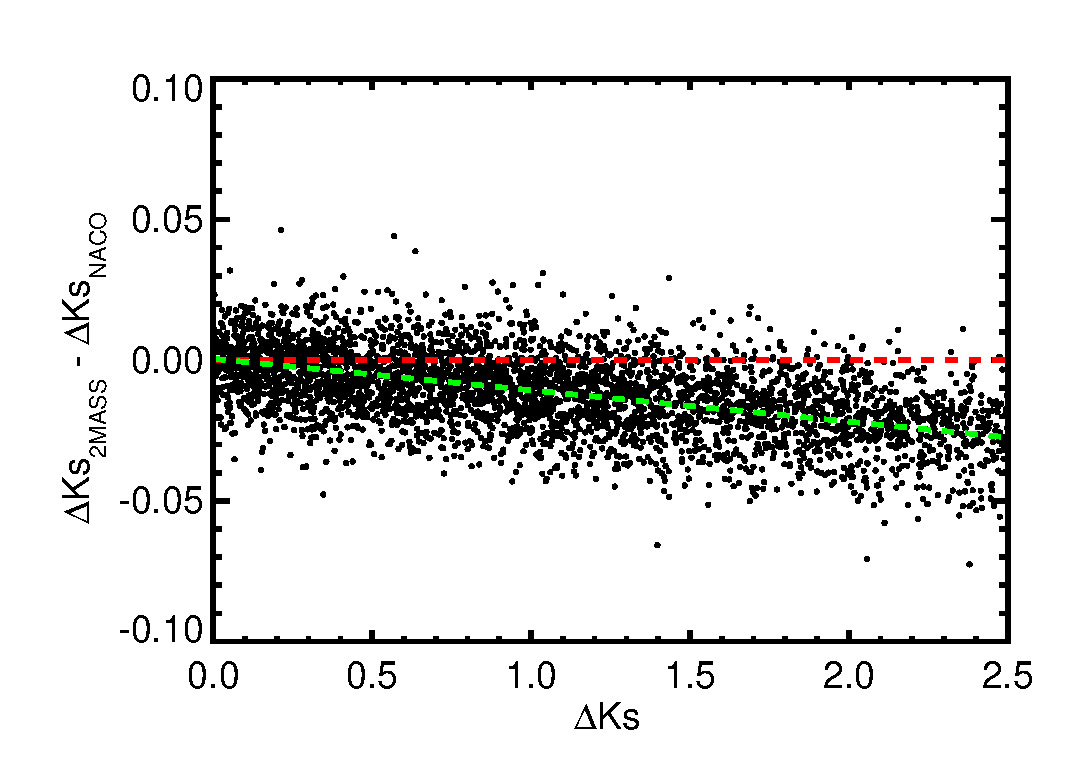
\includegraphics[width=0.47\textwidth]{NACO_Ks.eps}
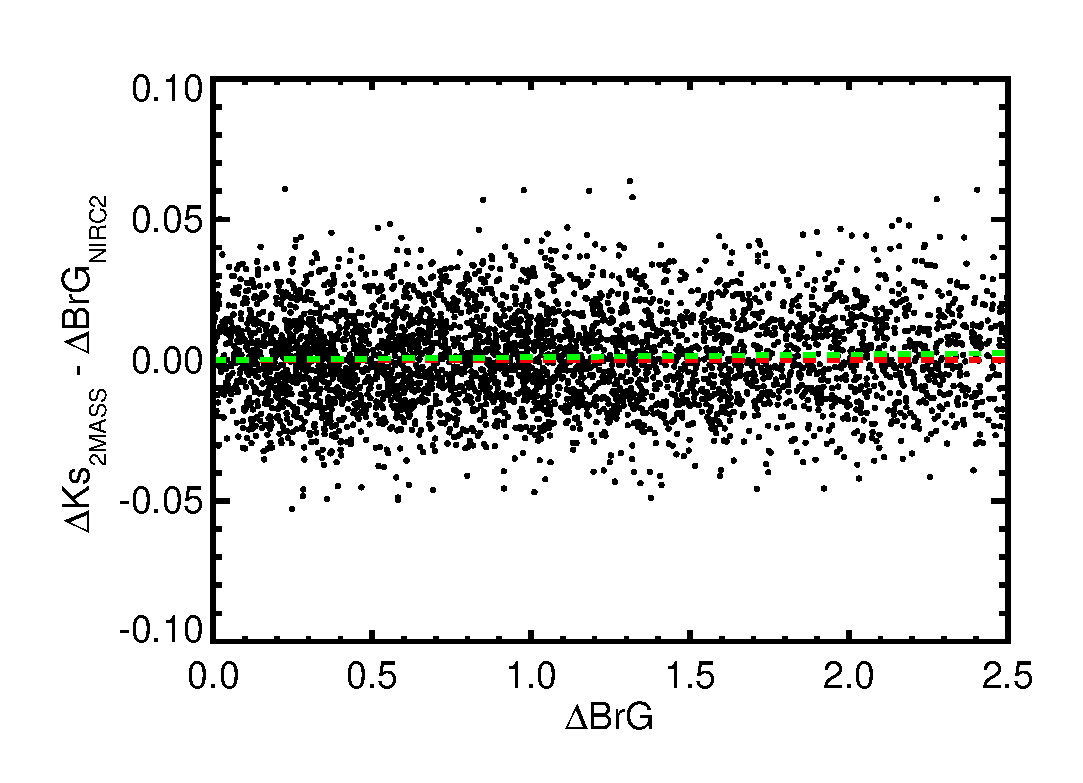
\includegraphics[width=0.47\textwidth]{NIRC2_BrG.eps}
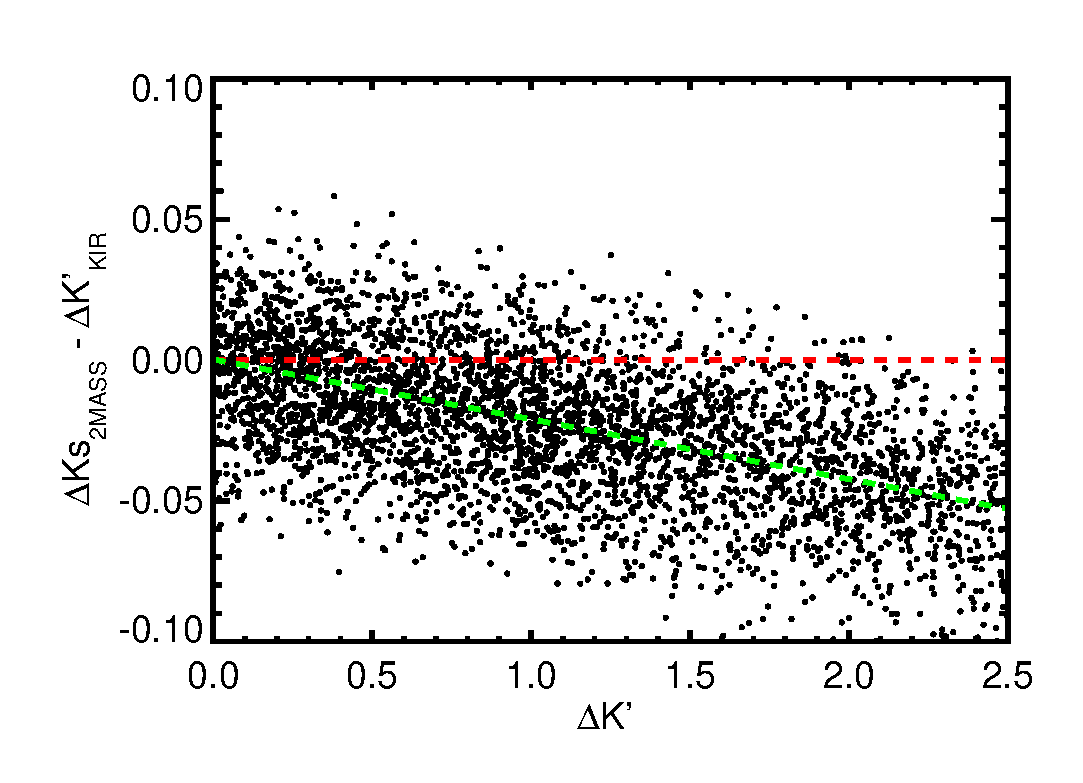
\includegraphics[width=0.47\textwidth]{KIR_Kp.eps}
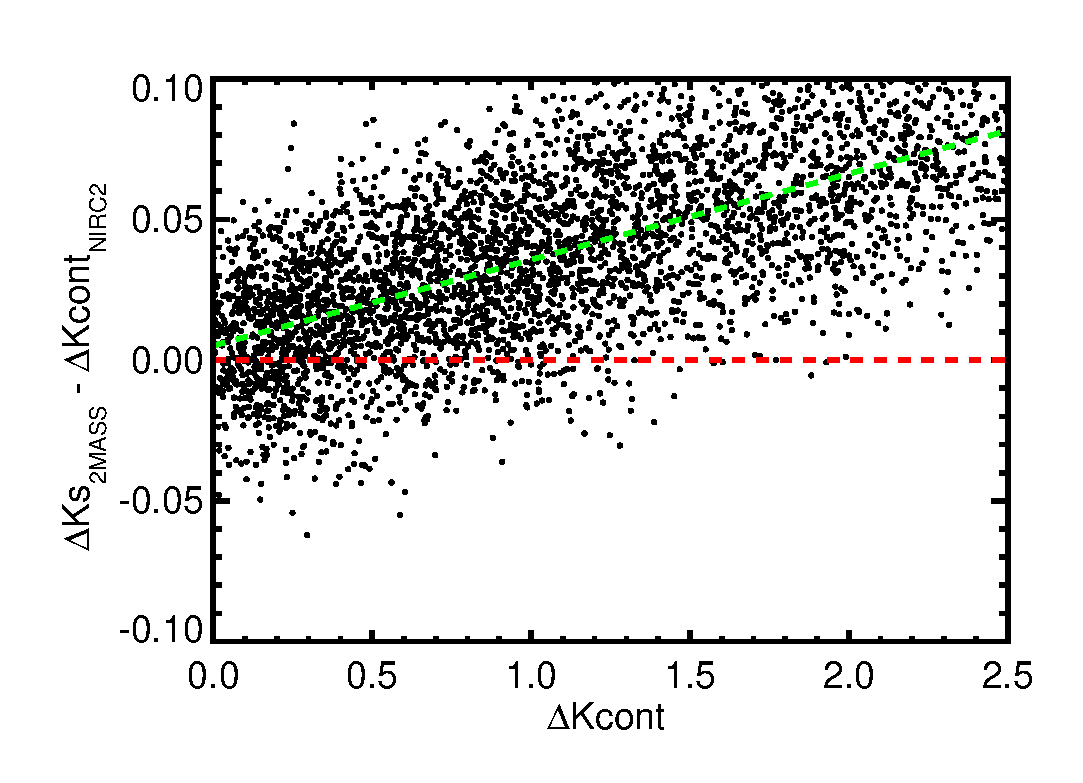
\includegraphics[width=0.47\textwidth]{NIRC2_Kcont.eps}
\caption{Difference between 2MASS $\Delta K_S$ and four example $\Delta$ magnitudes measured from our AO imaging, built from a grid of absolutely-calibrated spectra and the filter profiles provided for each filter. No corrections are applied for the NIRC2 Bracket-Gamma (BrG) and  $K_S$ (K-short) filter, as the trend is not significant compared to potential systematic issues in the calibration of the underlying spectra. }
\label{fig:mags}
\end{center}
\end{figure*}

We did not see a significant difference in any derived correction based on the metallicity of the component stars, as expected based on how [Fe/H] changes $K$-band flux levels (Figure~\ref{fig:metal}). Thus we did not attempt to include [Fe/H] in these relations. We also found no significant effect as a function of the mass of the primary. However, this was difficult to test due to limitations of the input sample. The \citet{Mann2015b} spectral sample covers K7 to M7, but is poorly populated on the extreme ends. While we can make a wide range of combinations of low-contrast systems (M0+M0 to M6+M6), we have limited options for high-contrast (where primary can only be $\sim$ K7-M1) systems where this effect is largest.

\section{Orbits of binaries}\label{sec:orbitplots}

Here we show diagnostic plots of each of the binaries analyzed in this paper. The three binaries shown in Figure~\ref{fig:orbits} are not repeated here. [FOR FILE SIZE REASONS I COMMENTED OUT THE ACTUAL FIGURES FOR NOW]

%\begin{figure*}[htp]
%\begin{center}
%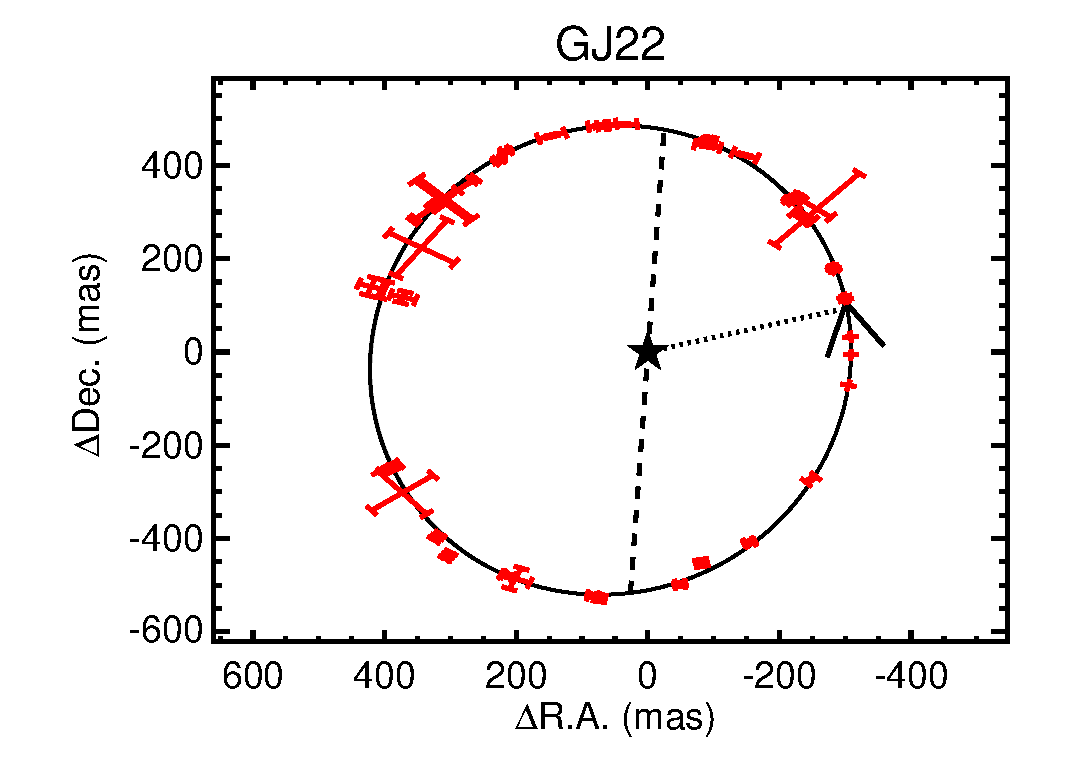
\includegraphics[width=0.32\textwidth]{Orbits/GJ22AB.eps}
%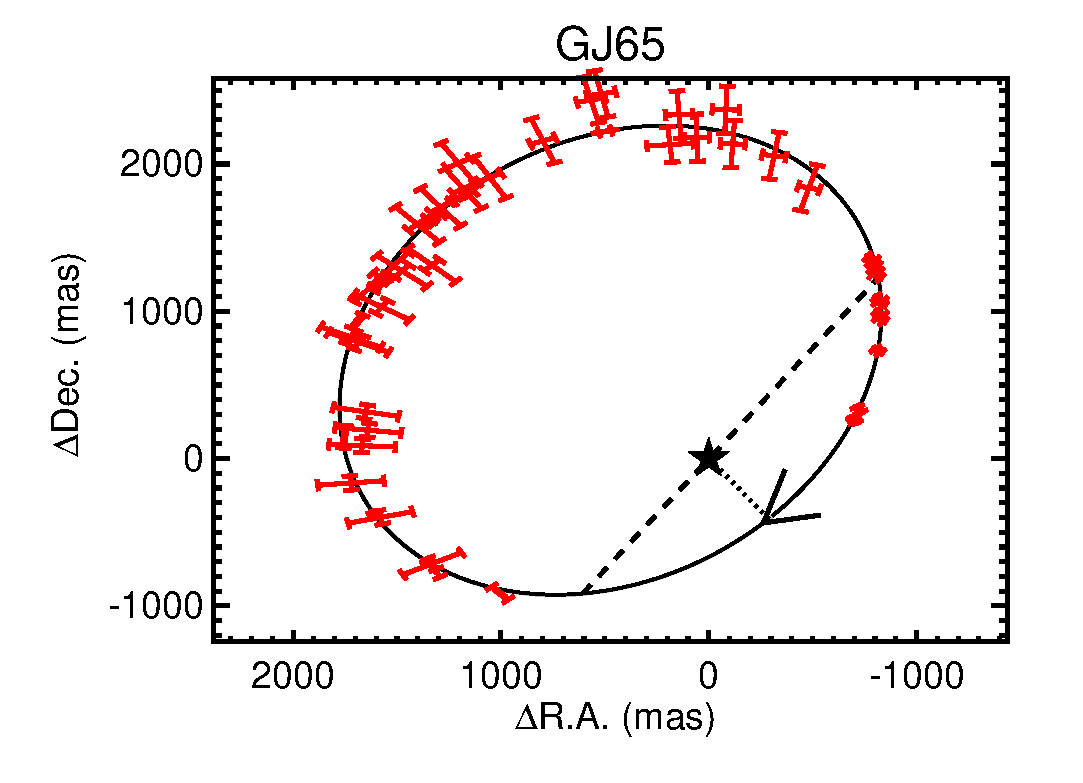
\includegraphics[width=0.32\textwidth]{Orbits/GJ65AB.eps}
%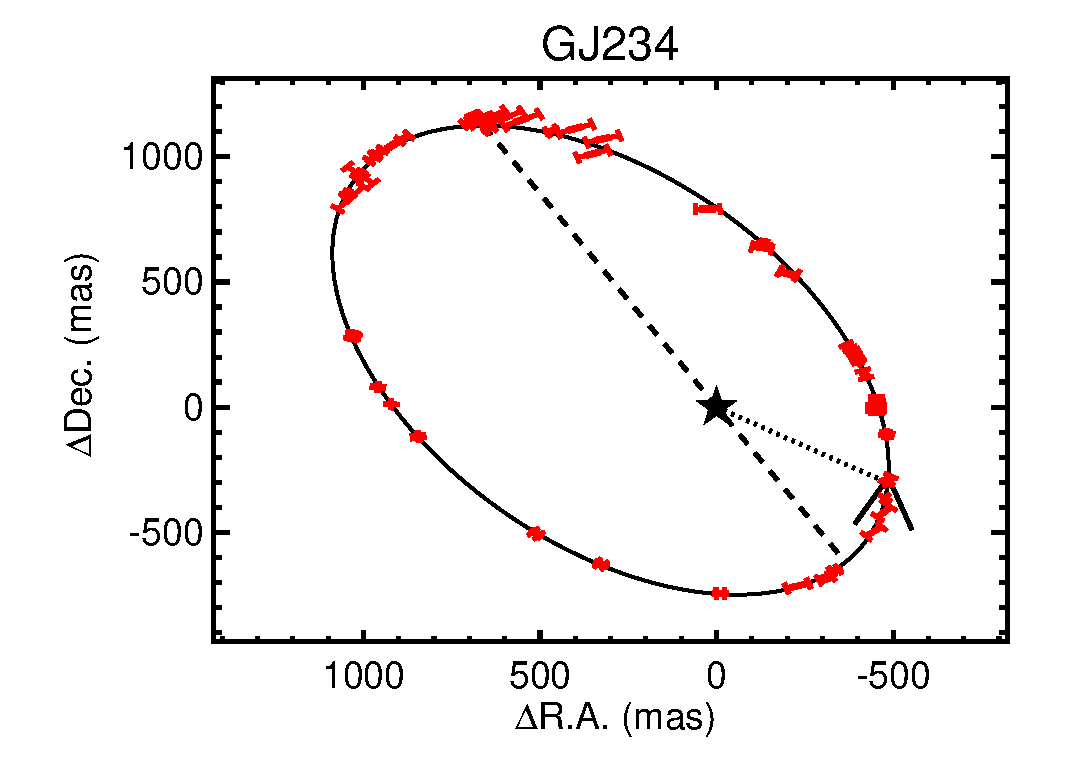
\includegraphics[width=0.32\textwidth]{Orbits/GJ234AB.eps}
%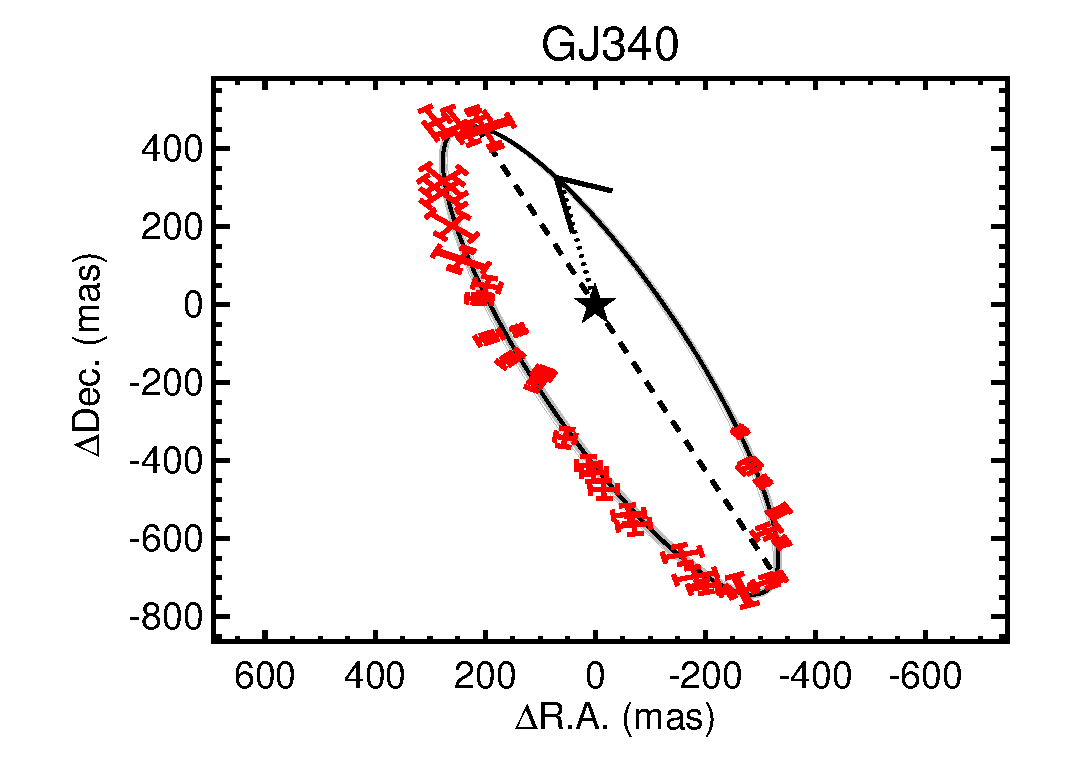
\includegraphics[width=0.32\textwidth]{Orbits/GJ340AB.eps}
%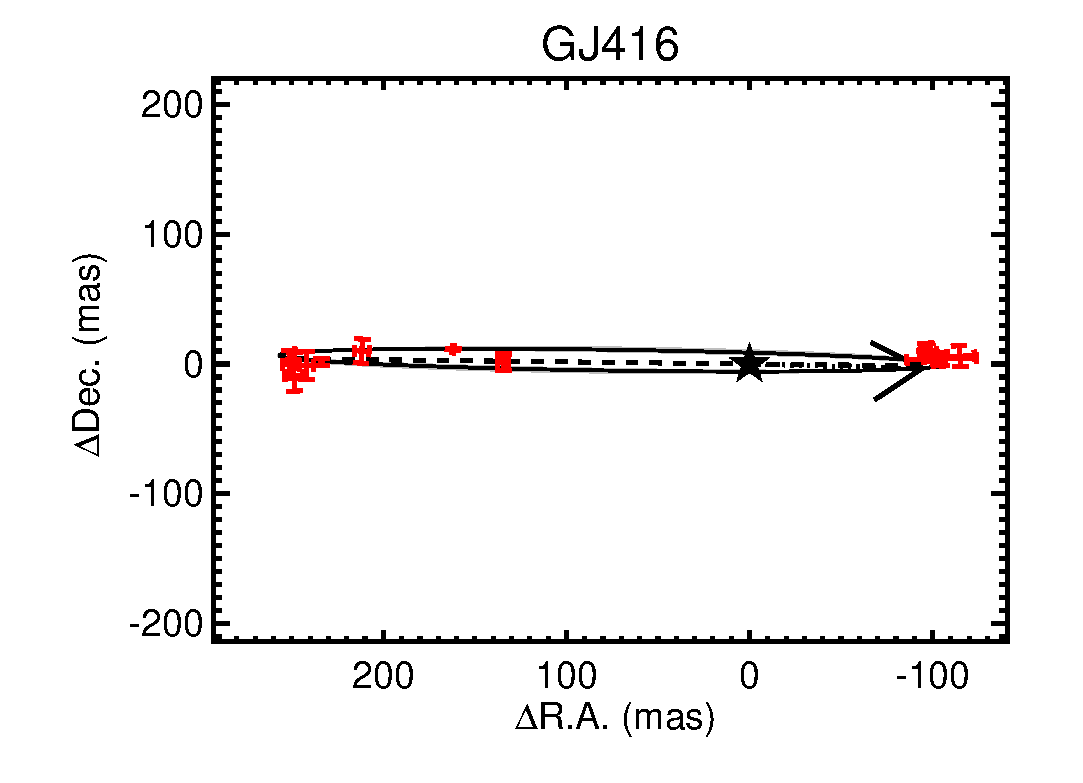
\includegraphics[width=0.32\textwidth]{Orbits/GJ416AB.eps}
%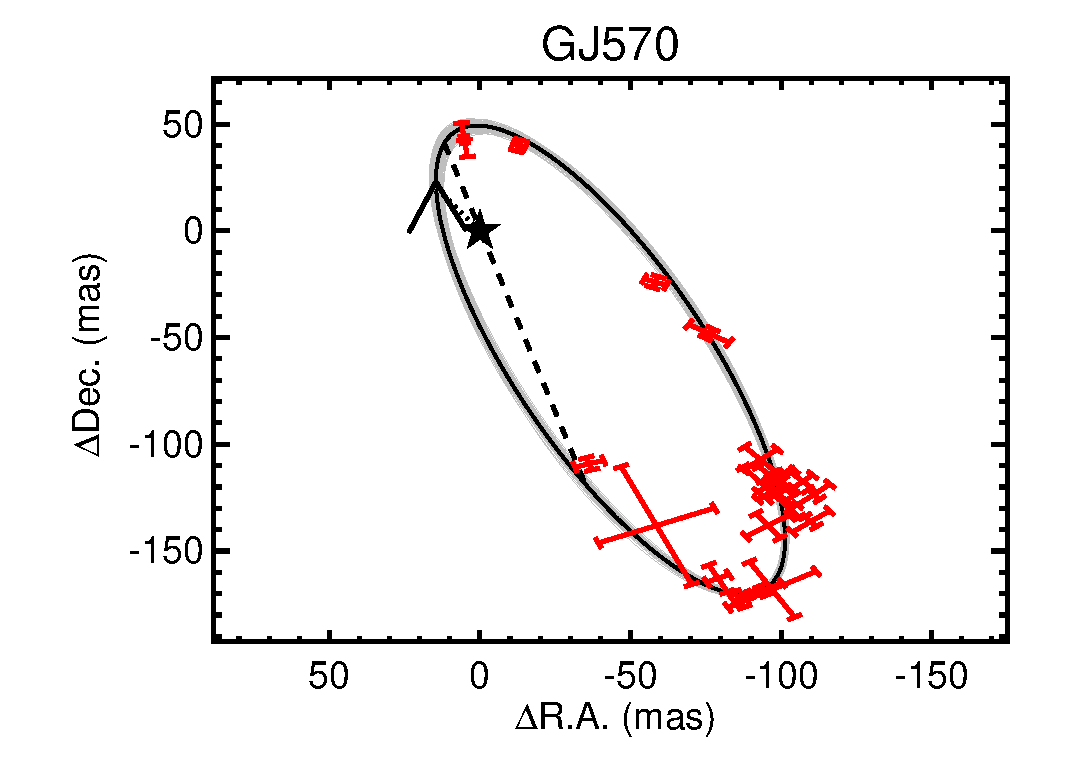
\includegraphics[width=0.32\textwidth]{Orbits/GJ570AB.eps}
%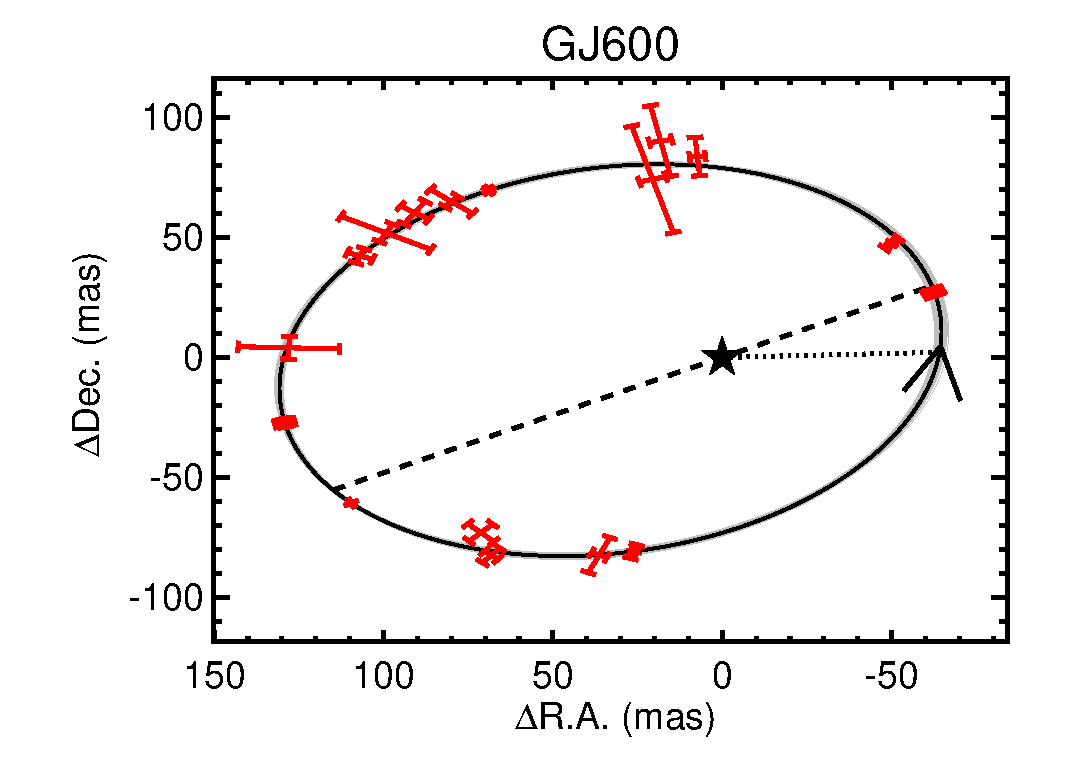
\includegraphics[width=0.32\textwidth]{Orbits/GJ600AB.eps}
%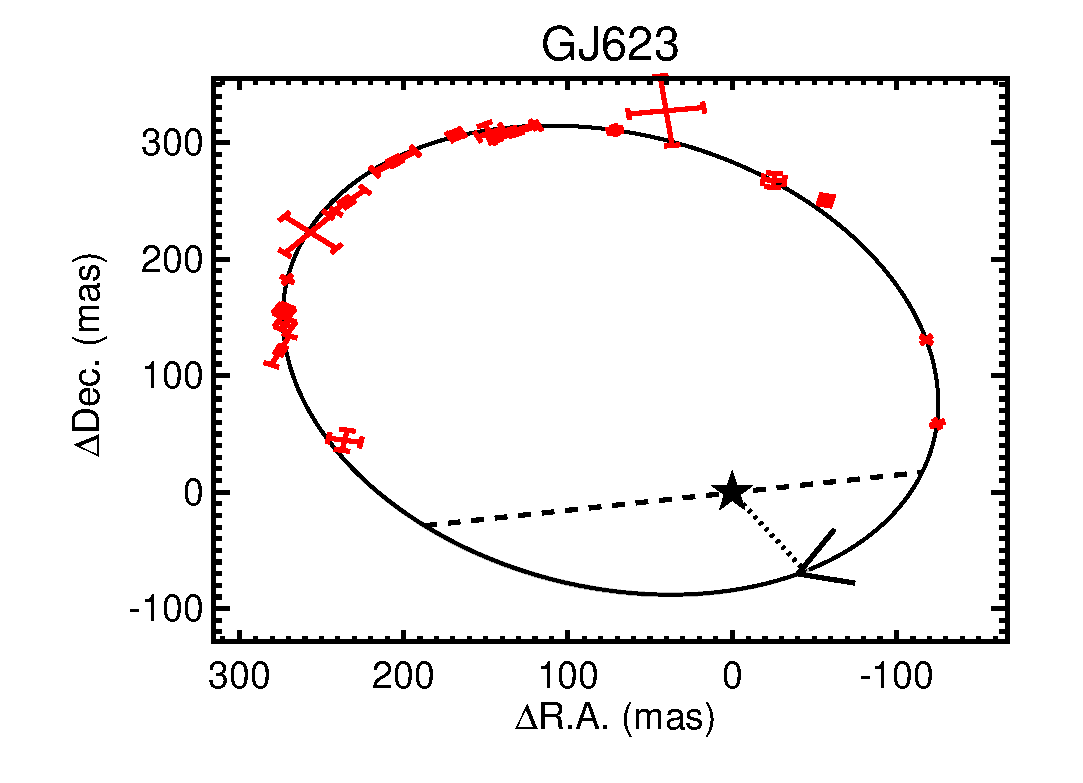
\includegraphics[width=0.32\textwidth]{Orbits/GJ623AB.eps}
%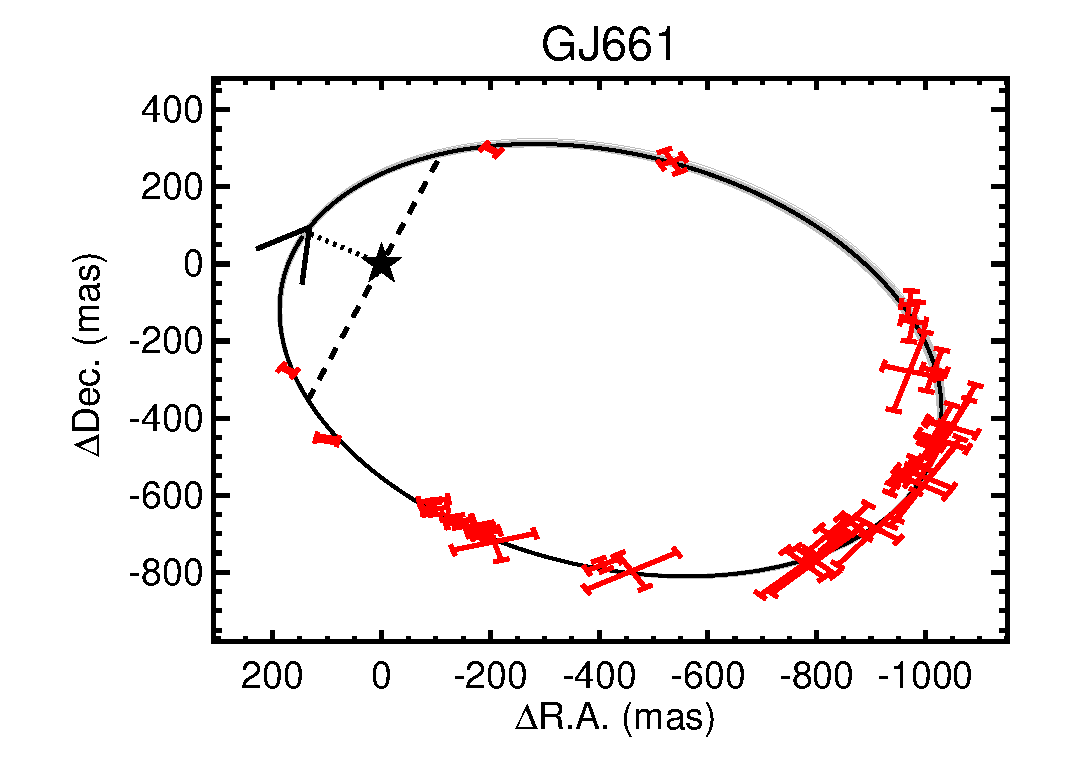
\includegraphics[width=0.32\textwidth]{Orbits/GJ661AB.eps}
%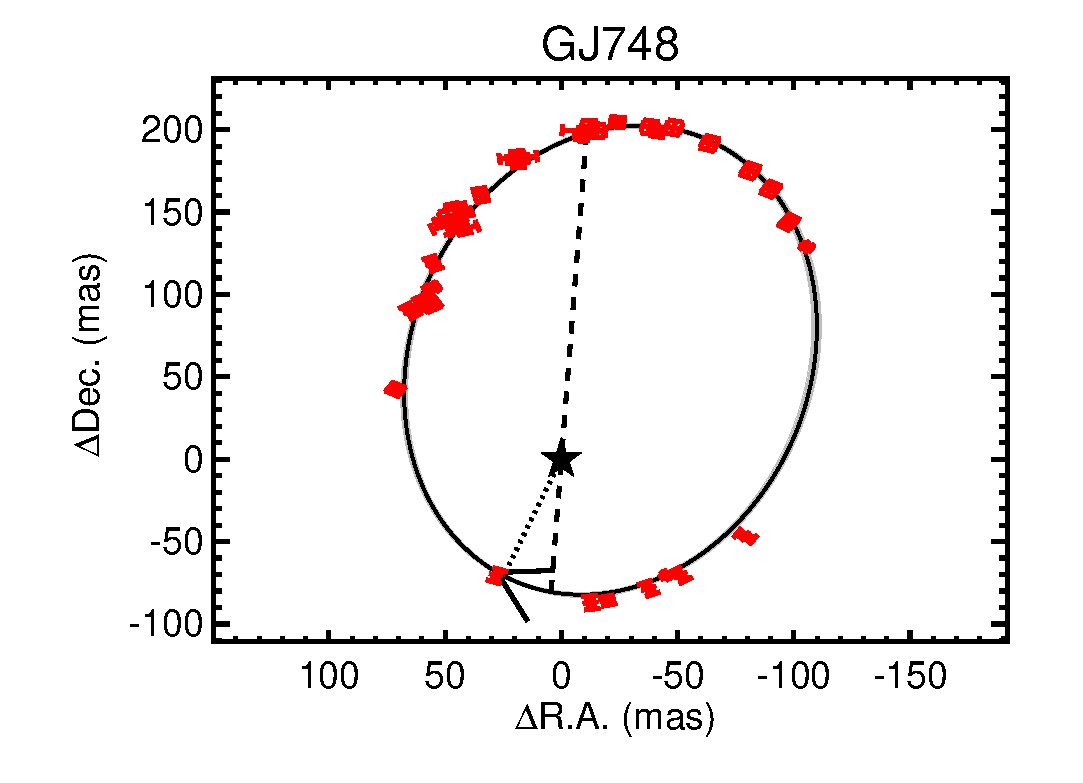
\includegraphics[width=0.32\textwidth]{Orbits/GJ748AB.eps}
%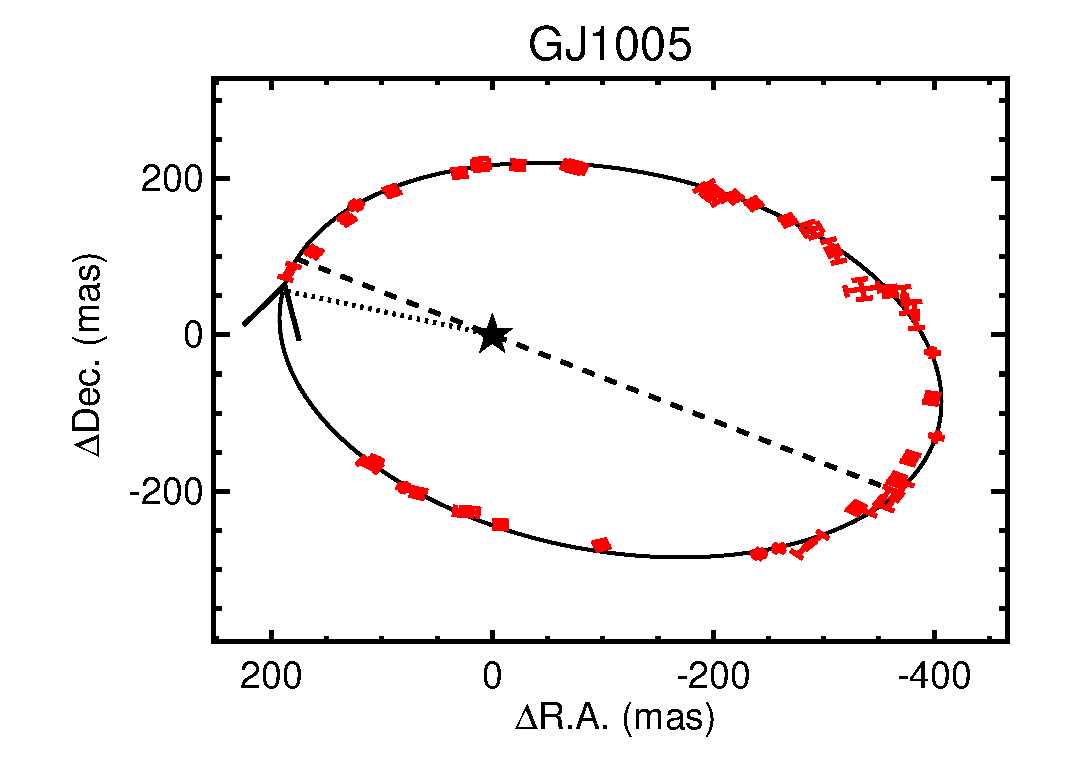
\includegraphics[width=0.32\textwidth]{Orbits/GJ1005AB.eps}
%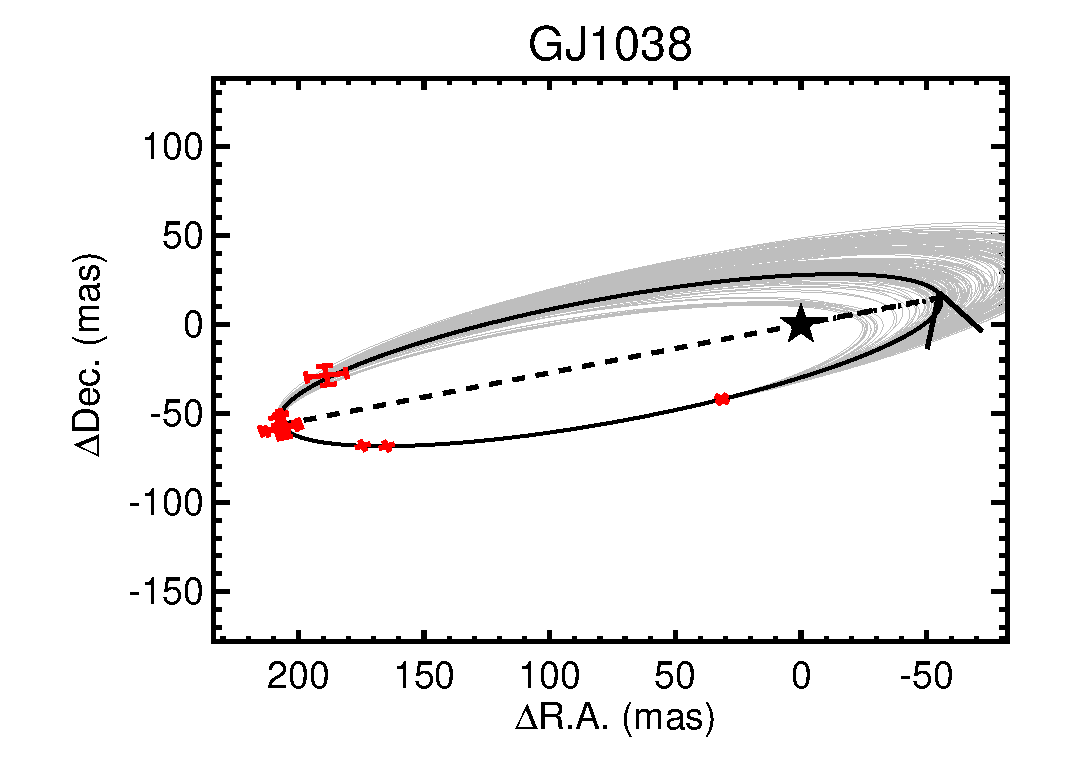
\includegraphics[width=0.32\textwidth]{Orbits/GJ1038AB.eps}
%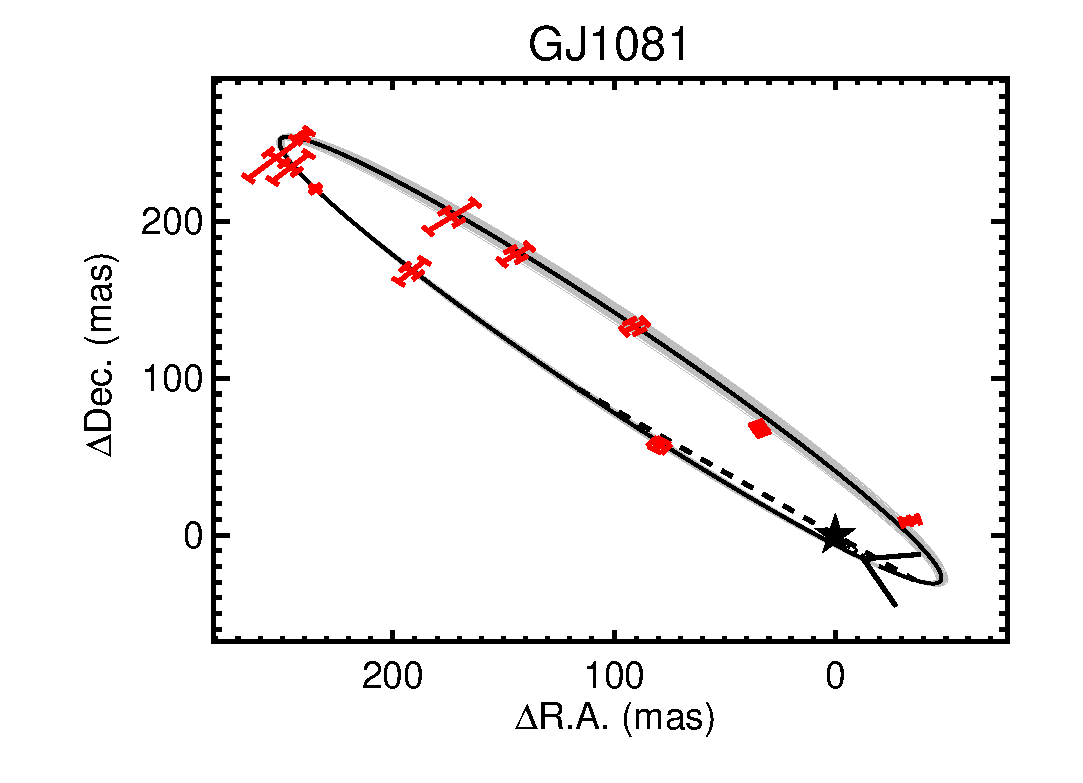
\includegraphics[width=0.32\textwidth]{Orbits/GJ1081AB.eps}
%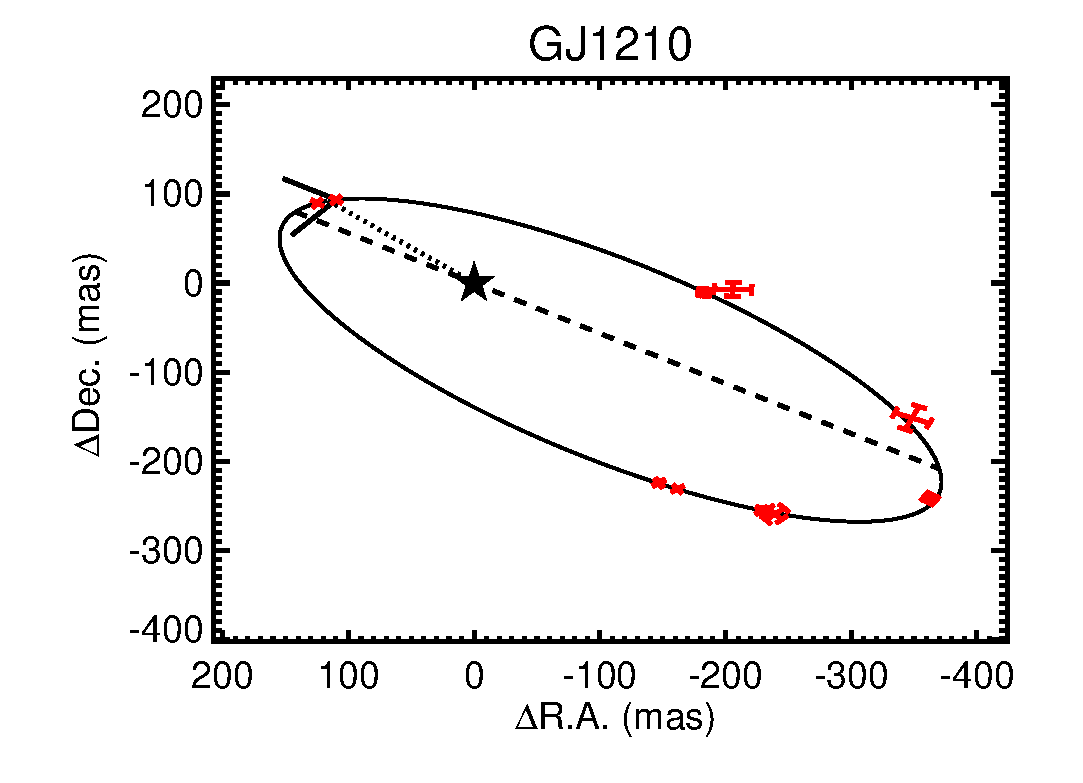
\includegraphics[width=0.32\textwidth]{Orbits/GJ1210AB.eps}
%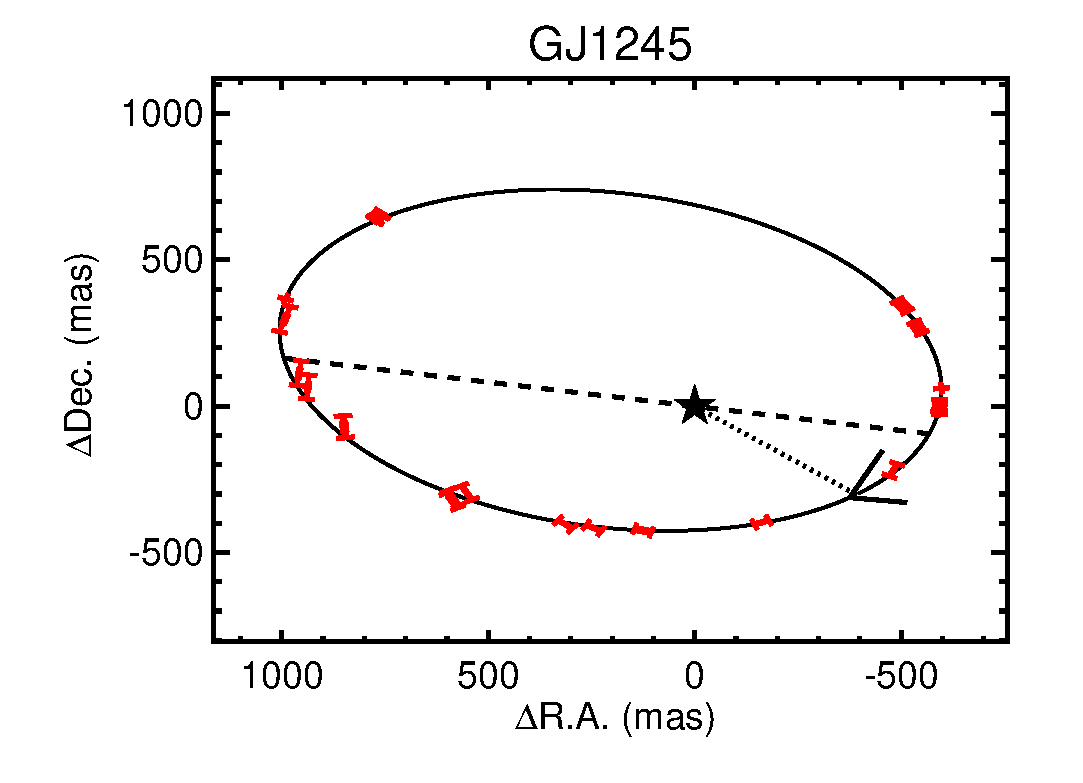
\includegraphics[width=0.32\textwidth]{Orbits/GJ1245AB.eps}
%\caption{Orbital fit for each binary fit in this paper in the reference frame of the primary. The black star marks the primary (always at 0, 0). The best-fit (highest likelihood) is shown as a black line, with 100 randomly selected orbit fits from the MCMC shown in grey. In many fits the thickness of the black line blocks much or all of the grey lines. Red points are individual measurements with adopted uncertainties. The dashed line is the line of nodes, the dotted line indicates periastron passage, and the arrow marks the direction of motion. }
%\label{fig:orbits1}
%\end{center}
%\end{figure*}
%
%\begin{figure*}[htp]
%\begin{center}
%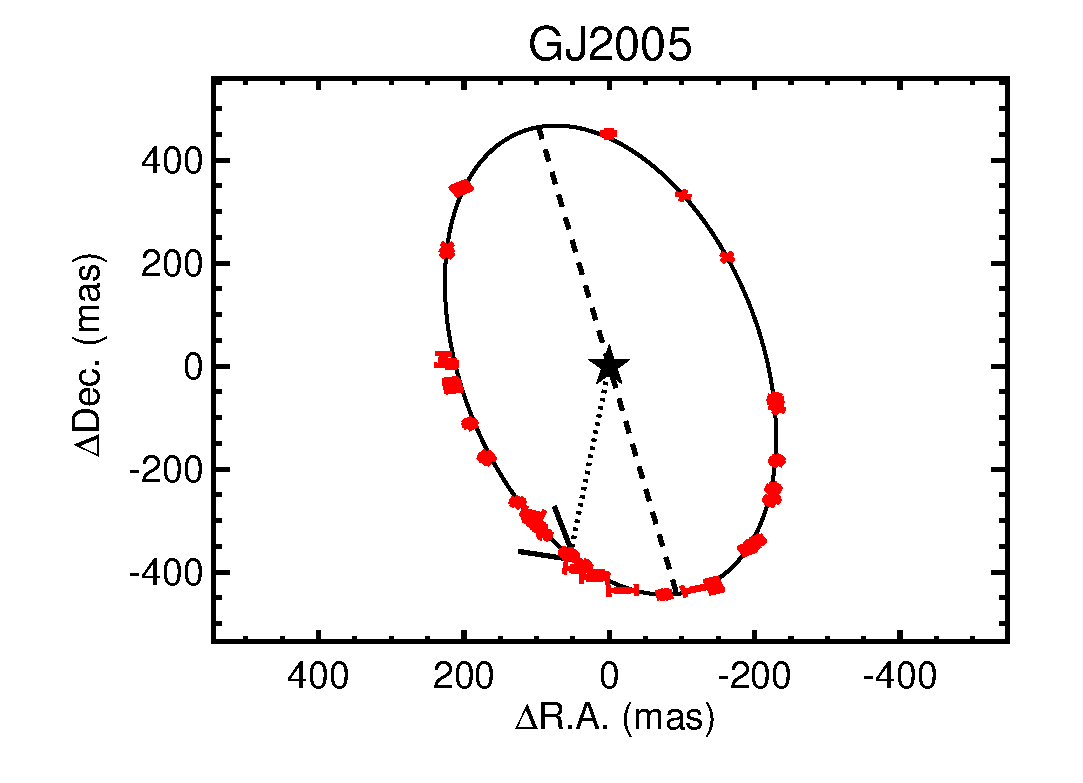
\includegraphics[width=0.32\textwidth]{Orbits/GJ2005AB.eps}
%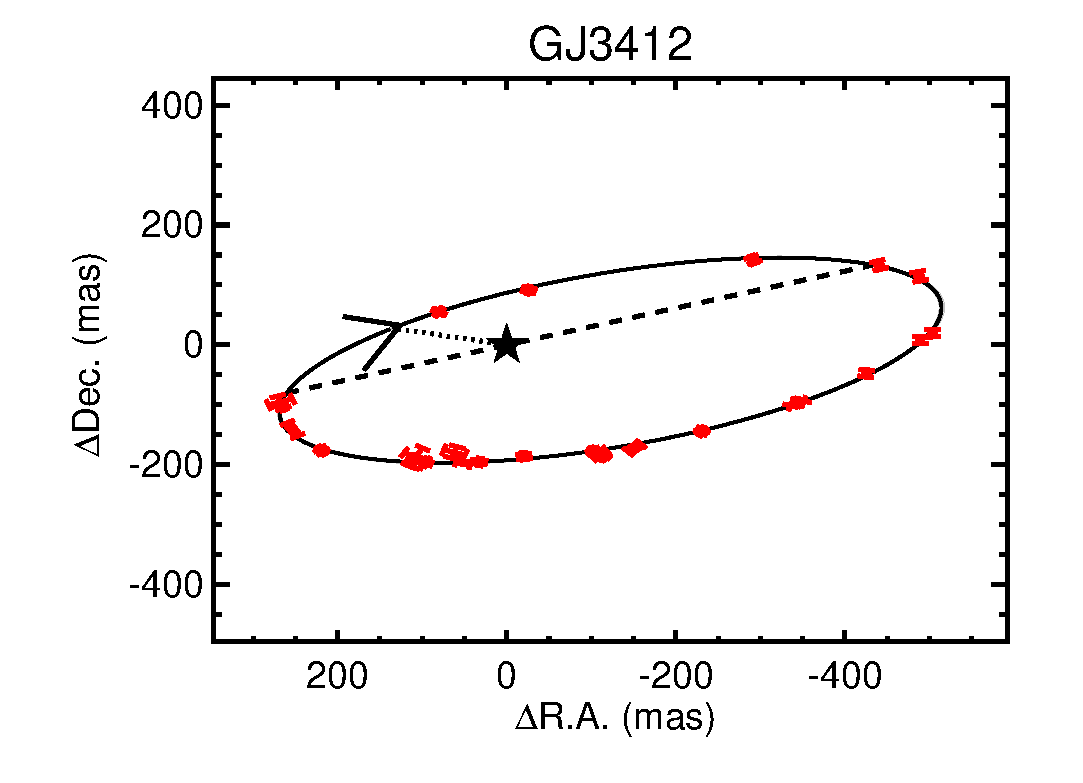
\includegraphics[width=0.32\textwidth]{Orbits/GJ3412AB.eps}
%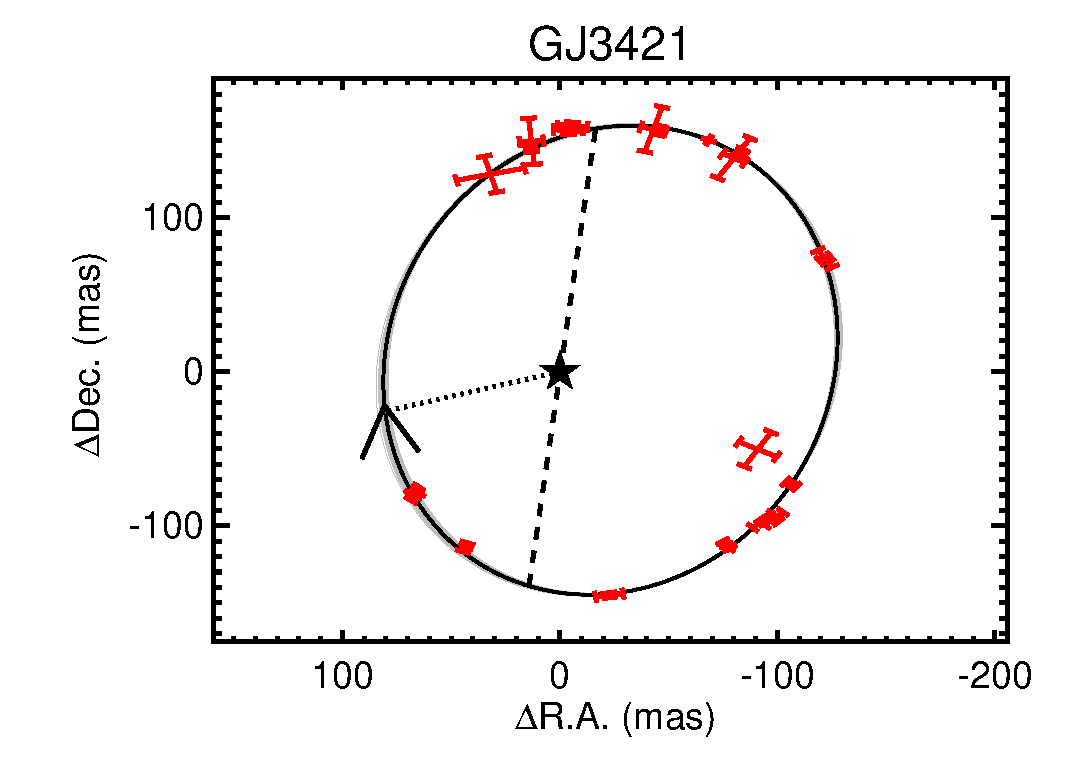
\includegraphics[width=0.32\textwidth]{Orbits/GJ3421AB.eps}
%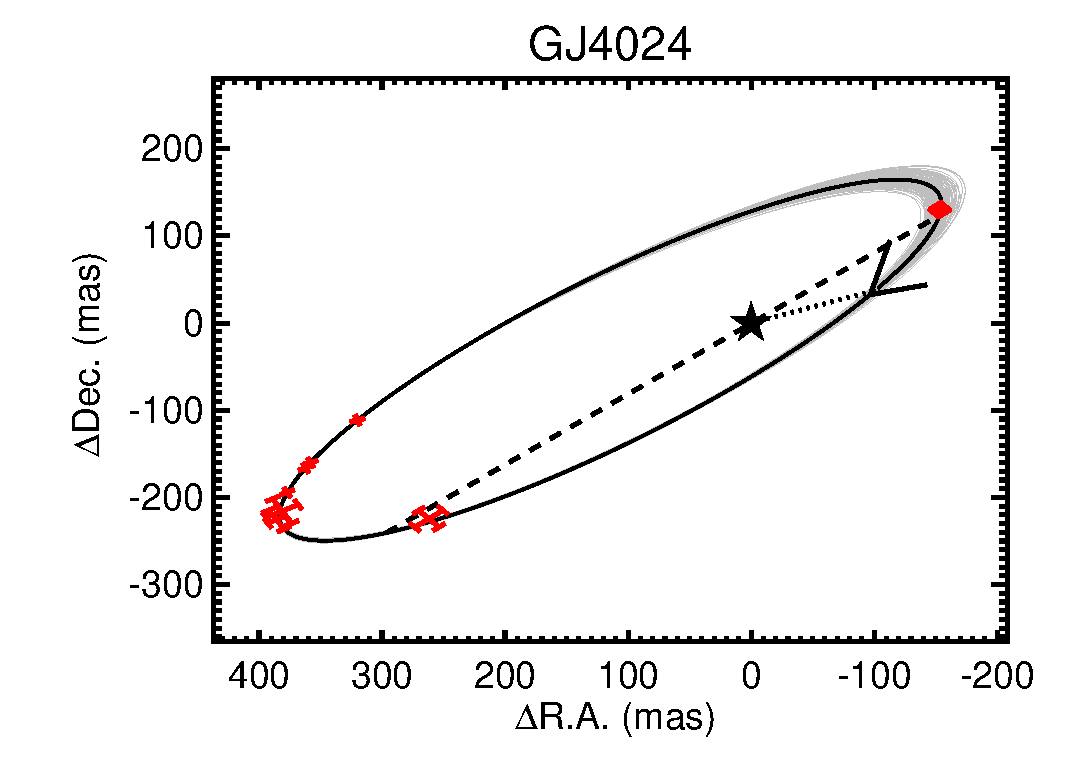
\includegraphics[width=0.32\textwidth]{Orbits/GJ4024AB.eps}
%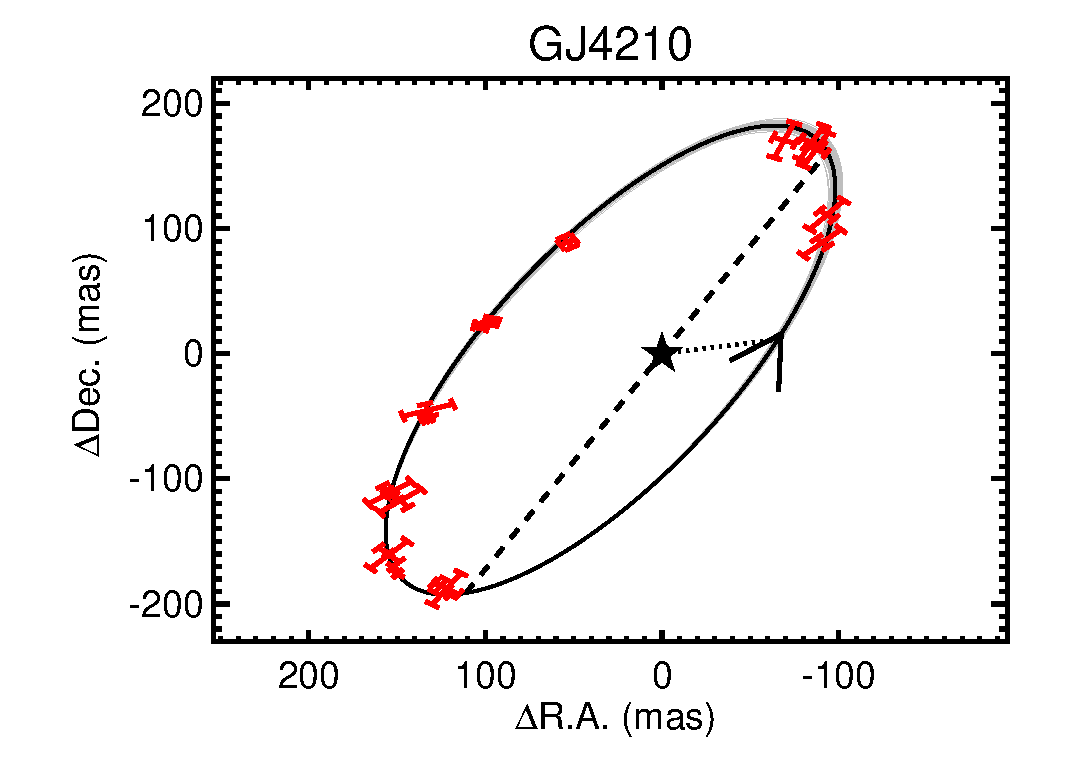
\includegraphics[width=0.32\textwidth]{Orbits/GJ4210AB.eps}
%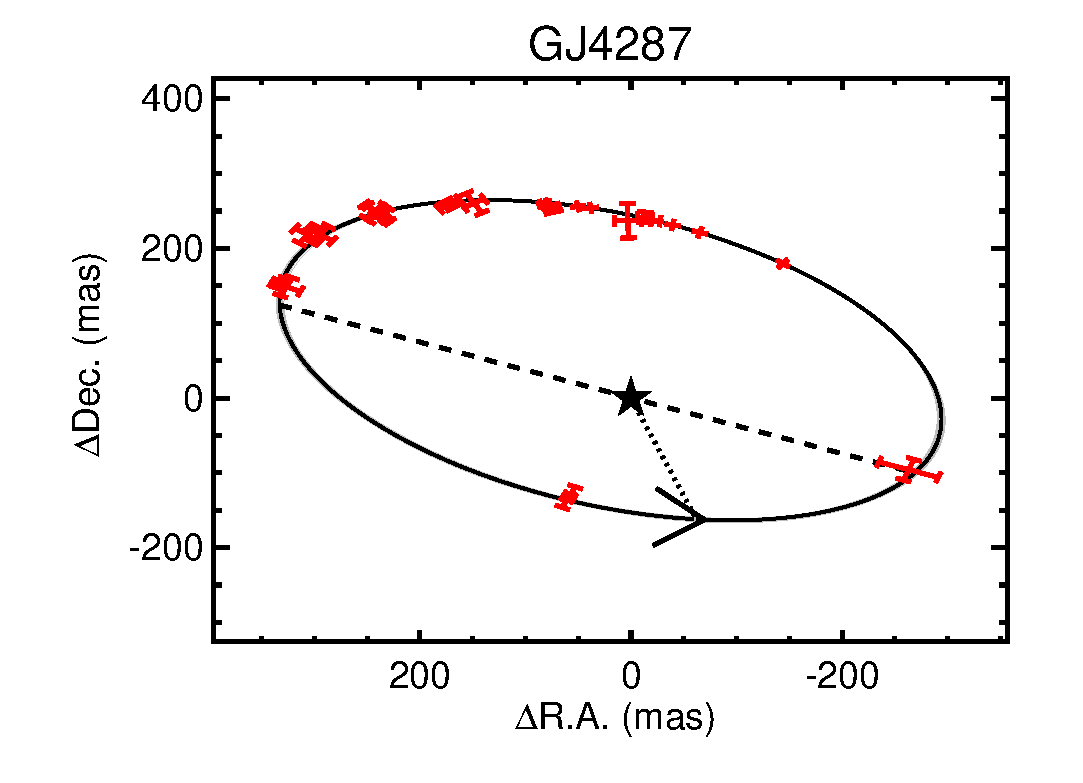
\includegraphics[width=0.32\textwidth]{Orbits/GJ4287AB.eps}
%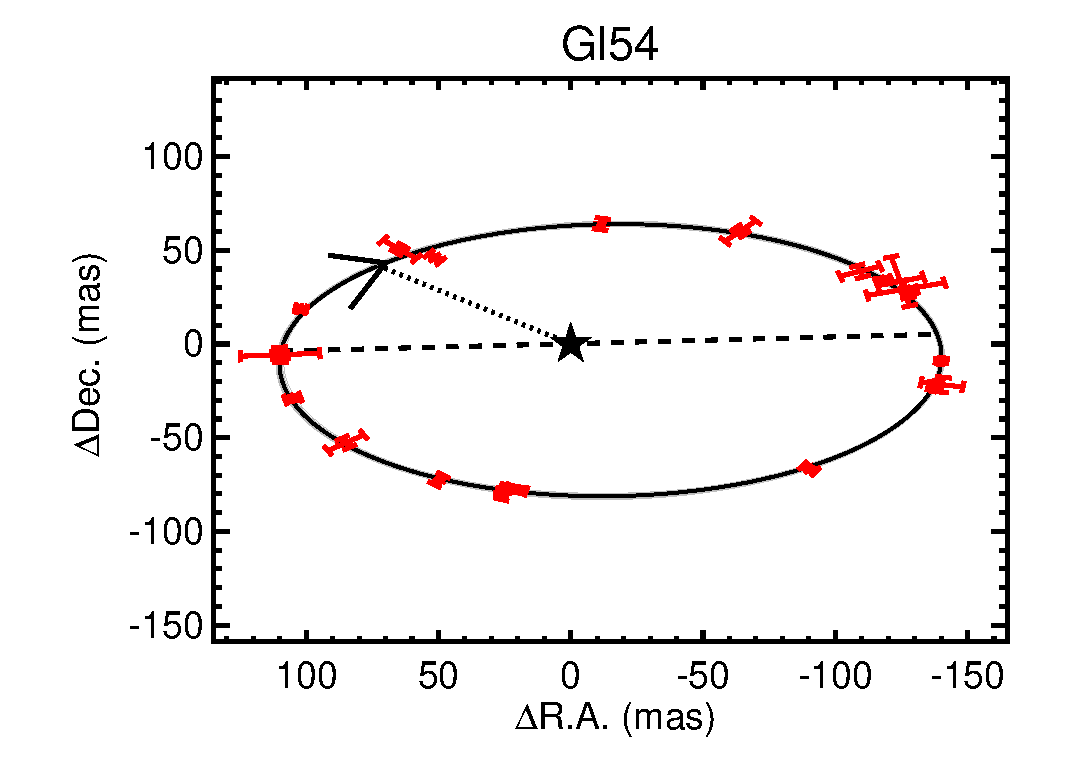
\includegraphics[width=0.32\textwidth]{Orbits/Gl54AB.eps}
%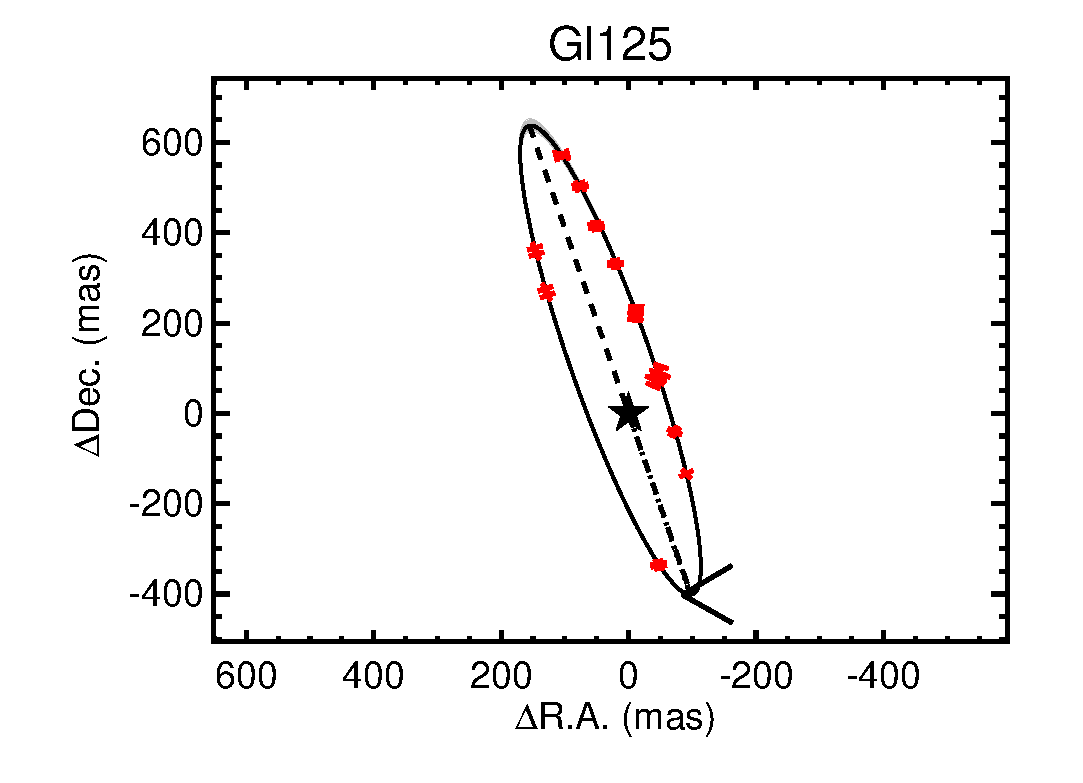
\includegraphics[width=0.32\textwidth]{Orbits/Gl125AB.eps}
%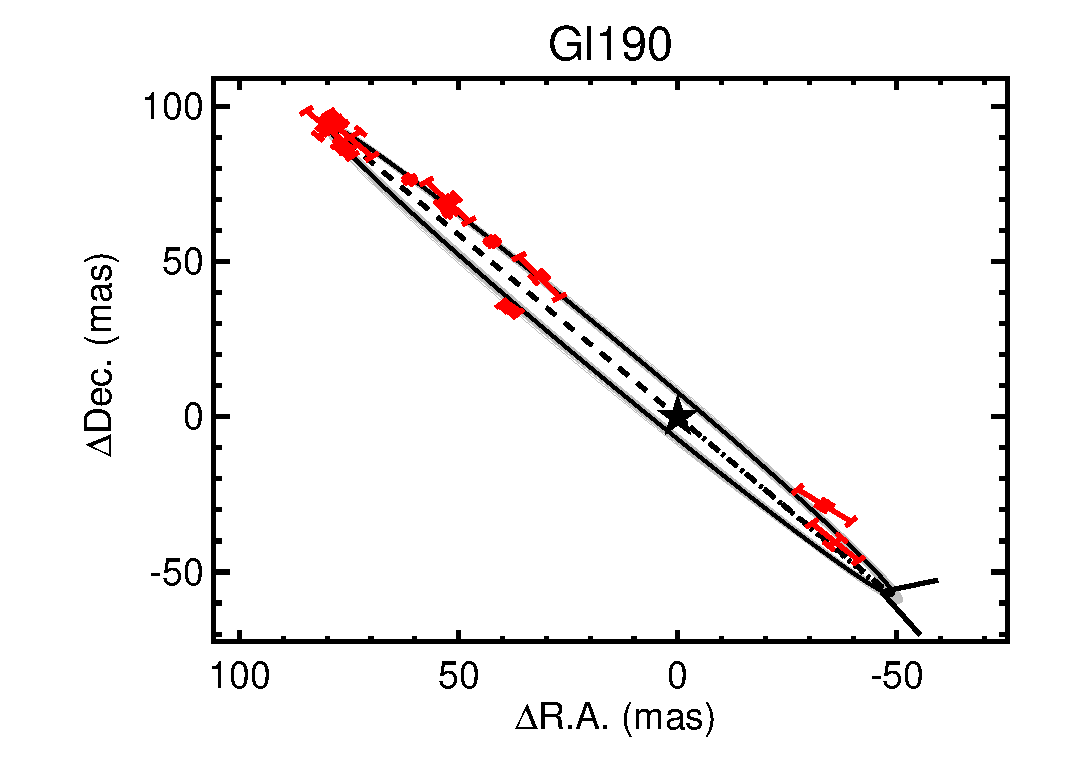
\includegraphics[width=0.32\textwidth]{Orbits/Gl190AB.eps}
%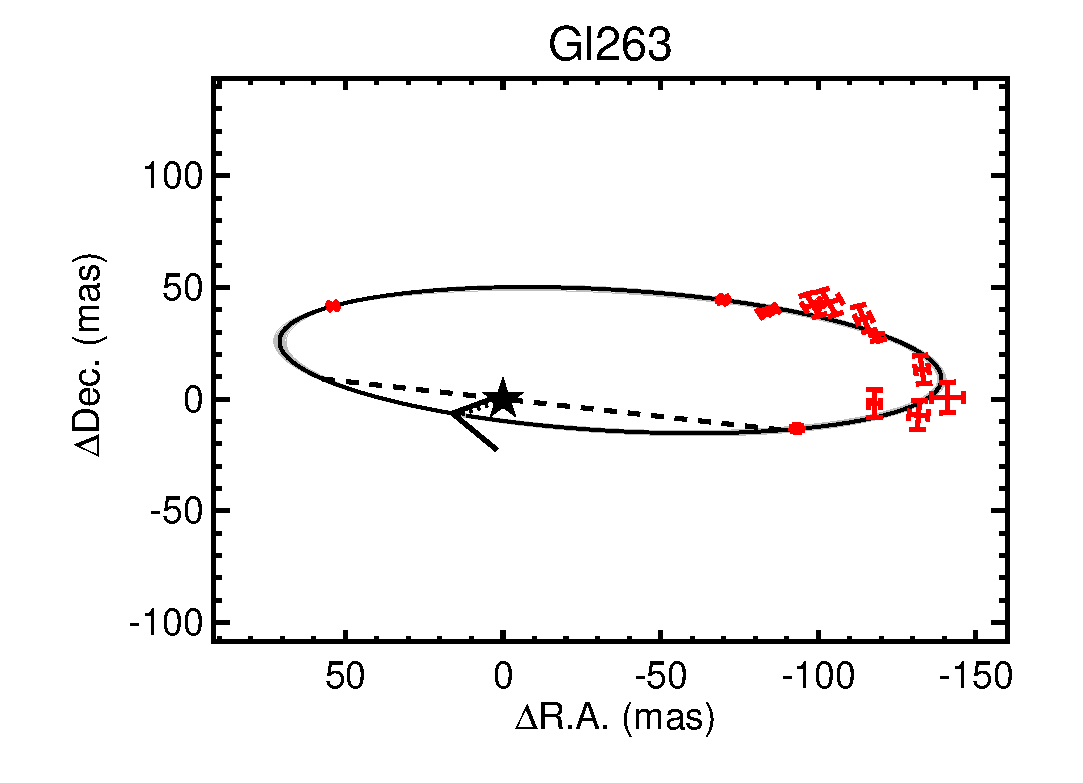
\includegraphics[width=0.32\textwidth]{Orbits/Gl263AB.eps}
%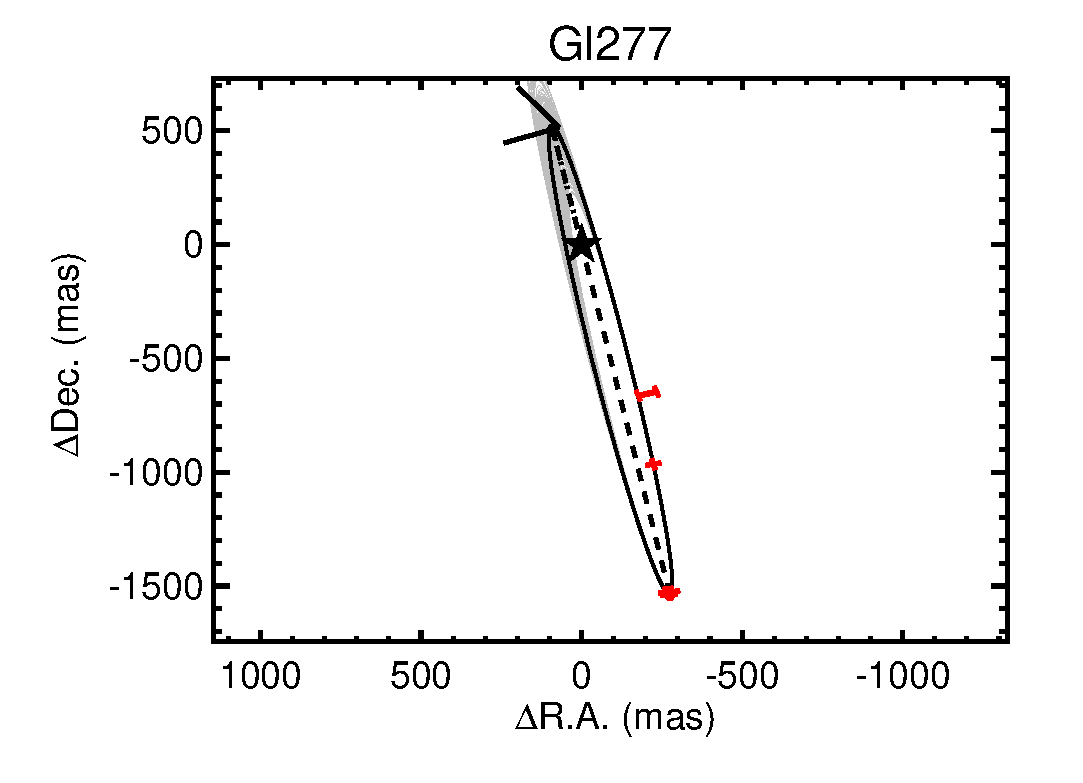
\includegraphics[width=0.32\textwidth]{Orbits/Gl277AB.eps}
%\includegraphics[width=0.32\textwidth]{Orbits/Gl310AB.eps}
%\includegraphics[width=0.32\textwidth]{Orbits/Gl330AB.eps}
%\includegraphics[width=0.32\textwidth]{Orbits/Gl381AB.eps}
%\includegraphics[width=0.32\textwidth]{Orbits/Gl473AB.eps}
%\caption{Figure~\ref{fig:orbits1} continued.}
%\label{fig:orbits2}
%\end{center}
%\end{figure*}
%
%
%\begin{figure*}[htp]
%\begin{center}
%\includegraphics[width=0.32\textwidth]{Orbits/Gl494AB.eps}
%\includegraphics[width=0.32\textwidth]{Orbits/Gl660AB.eps}
%\includegraphics[width=0.32\textwidth]{Orbits/Gl695AB.eps}
%\includegraphics[width=0.32\textwidth]{Orbits/Gl747AB.eps}
%\includegraphics[width=0.32\textwidth]{Orbits/Gl7912AB.eps}
%\includegraphics[width=0.32\textwidth]{Orbits/Gl804AB.eps}
%\includegraphics[width=0.32\textwidth]{Orbits/Gl831AB.eps}
%\includegraphics[width=0.32\textwidth]{Orbits/Gl844AB.eps}
%\includegraphics[width=0.32\textwidth]{Orbits/Gl8934AB.eps}
%\includegraphics[width=0.32\textwidth]{Orbits/Gl913AB.eps}
%\includegraphics[width=0.32\textwidth]{Orbits/HD15285AB.eps}
%\includegraphics[width=0.32\textwidth]{Orbits/HD239960AB.eps}
%\includegraphics[width=0.32\textwidth]{Orbits/HIP9724AB.eps}
%\includegraphics[width=0.32\textwidth]{Orbits/HIP11542AB.eps}
%\includegraphics[width=0.32\textwidth]{Orbits/HIP46706AB.eps}
%\caption{Figure~\ref{fig:orbits1} continued.}
%\label{fig:orbits3}
%\end{center}
%\end{figure*}
%
%\begin{figure*}[htp]
%\begin{center}
%\includegraphics[width=0.32\textwidth]{Orbits/HIP95995AB.eps}
%\includegraphics[width=0.32\textwidth]{Orbits/HIP96656AB.eps}
%\includegraphics[width=0.32\textwidth]{Orbits/LHS6167AB.eps}
%\includegraphics[width=0.32\textwidth]{Orbits/PMJ02133+3648AB.eps}
%\includegraphics[width=0.32\textwidth]{Orbits/Gl301AB.eps}
%\includegraphics[width=0.32\textwidth]{Orbits/Gl469AB.eps}
%\includegraphics[width=0.32\textwidth]{Orbits/GJ3454AB.eps}
%\caption{Figure~\ref{fig:orbits1} continued.}
%\label{fig:orbits4}
%\end{center}
%\end{figure*}

\end{document}


